%% main_ppgco_ufu.tex v1.0, Lásaro Camargos e Denise Guliato
% adaptado de modeloABNT2.tex, v1.0 athila 
% ------------------------------------------------------------------------
% ------------------------------------------------------------------------
% eesc: Modelo de Trabalho Acadêmico (tese de doutorado, dissertação de
% mestrado e trabalhos monográficos em geral) em conformidade com 
% ABNT NBR 14724:2011. Esta classe estende as funcionalidades da classe
% abnTeX2 elaborada de forma a adequar os parâmetros exigidos pelas 
% normas USP e do departamento de elétrica da Escola de Engenharia 
% de São Carlos - USP.
% ------------------------------------------------------------------------
% ------------------------------------------------------------------------

% ------------------------------------------------------------------------
% Opções:
% 	tesedr:     Formata documento para tese de doutorado
%	qualidr:    Formata documento para qualificação de doutorado
% 	dissertmst: Formata documento para dissertação de mestrado
% 	qualimst:   Formata documento para qualificação de mestrado
% ------------------------------------------------------------------------

\documentclass[dissertmst]{ppgco}

%Não altere o comando seguinte. O título de seu trabalho será especificado mais adiante.
\title{Template de Monografia do PPGCO}
%\let\cleardoublepage\clearpage

% Pacotes essenciais
\usepackage{lmodern}
\usepackage[T1]{fontenc}
\usepackage[utf8]{inputenc}
\usepackage[brazil]{babel}
\usepackage[printonlyused]{acronym}

% Tipografia
\usepackage{microtype}

% Matemática
\usepackage{amsmath}

% Figuras
\usepackage{graphicx}

% Tabelas
\usepackage{booktabs}
\usepackage{multirow}
\usepackage[table,xcdraw]{xcolor}
\usepackage{makecell}
\usepackage{graphicx}

% Algoritmos
\usepackage{algorithm}
\usepackage{algorithmic}

% Índices
\usepackage{makeidx}
\usepackage{nomencl}

% Qualidade
\usepackage{indentfirst}
\usepackage{float}

% Usado pela Ficha catalográfica
\usepackage{lastpage}	

% Define um padrão para 'caption' em imagens e tabelas
\usepackage[font=small,labelfont=bf]{caption} 		

% Links (sempre por último)
\usepackage{hyperref}

% Caminho pré definido de imagens
\graphicspath{
	{figuras/}
	{figuras/figs_fundamentacao/}
	{figuras/figs_metodologia/}
	{figuras/figs_experimentos/}
}

\makeatletter

\renewcommand{\printchapternonum}{%
	\vspace*{-3cm}%
}

\makeatother

% ==================================================================
% Informações de dados para CAPA e FOLHA DE ROSTO
% ==================================================================
%
% Título:
%	1. Título em português
%	2. Título em inglês
\titulo{Avaliação de Dor em Camundongos com Redes Neurais e Visão Computacional}{Pain Assessment in Mice with Neural Networks and Computer Vision}
%
% Autor:
%	1. Nome completo do autor
%	2. Formato de nome para bibliografia
\autor{Marcio Salmazo Ramos}{Sobrenome, Nome}
%
% Cidade
\local{Uberlândia}
% Ano de defesa
\data{2025}
% Área de concentração da pesquisa
\areaconcentracao{Ciência da Computação}
% Nome do orientador
\orientador{Maurício Cunha Escarpinati}
% Nome do coorientador
\coorientador{Daniel Duarte Abdala}

% ==================================================================
% compila o indice
% ==================================================================
\makeindex

% ==================================================================
% Compila a lista de abreviaturas e siglas
% ==================================================================

\makenomenclature

% ==================================================================
% Inserir ficha catalográfica
% ==================================================================
%
% Caso o comando \inserirfichacatalografica seja definido, a %ficha catalográfica
% será inserida atrás da folha de rosto. Caso contrário a página será deixada em
% branco.
%
% CUIDADO: Esta opção deve ser preenchida antes do comando \maketitle
% entre em contato com a biblioteca para obter a sua ficha catalográfica em arquivo pdf.  
% Essa folha só será inserida no documento após a sua defesa.

\inserirfichacatalografica{auxiliares/FichaCatalografica.pdf}

% ==================================================================
% Inserir folha de aprovação
% ==================================================================

% Caso o comando \inserirfolhaaprovacao seja definido, a a folha de aprovação
% será inserida. Além disso, conforme Resolução CoPGr 5890, as informações 
% de rodapé são inseridas apropriadamente na folha de rosto.
%
% CUIDADO: Esta opção deve ser preenchida antes do comando \maketitle
% baseie-se no modelo desse documento e gere a sua folha de %rosto em arquivo pdf.

\inserirfolhaaprovacao{auxiliares/Ata.pdf}

% ==================================================================
% Início do documento
% ==================================================================-
\begin{document}

\clearpage
\pagenumbering{arabic}
\sloppy

% ----------------------------------------------------------
% Insere Capa, Folha de rosto, Ficha catalográfica 
% (se inserida) e folha de aprovação (se inserida).
% ----------------------------------------------------------
\pretextual
\maketitle


% ----------------------------------------------------------
% Dedicatória
% ----------------------------------------------------------
\imprimirdedicatoria{
		Este trabalho é dedicado inteiramente a Deus.\\
		Por Sua graça, direção e providência, tudo se torna possível.
	}

% ----------------------------------------------------------
% Agradecimentos
% ----------------------------------------------------------
\imprimiragradecimentos{
	
	Agradeço primeiramente a Deus, por sua presença constante em minha vida, pelas bênçãos concedidas ao longo desta trajetória e pela força necessária para superar os desafios encontrados durante a realização deste trabalho. Sua providência e cuidado foram fundamentais para que eu pudesse chegar até este momento.
	
	Aos meus pais, agradeço imensamente pelo amor, apoio e incentivo ao longo de toda minha formação acadêmica e pessoal. Em todos os momentos, especialmente nos mais difíceis, eles foram fonte de motivação, confiança e inspiração para que eu continuasse seguindo em frente. Por isso, digo com toda a convicção que eles foram e continuam sendo o meu porto seguro.
	
	Estendo também os agradecimentos aos meus orientadores, pela paciência, disponibilidade e pelos valiosos ensinamentos compartilhados durante o desenvolvimento desta pesquisa, inclusive, por despertaram em mim o interesse pela pesquisa científica. Adicionalmente, agradeço a todos os professores que fizeram parte da minha trajetória acadêmica. Cada disciplina ministrada, cada conselho oferecido e cada oportunidade de aprendizado contribuíram diretamente para a construção do conhecimento que me permitiu alcançar esta etapa. 
	
	Agradeço ainda aos profissionais e colaboradores que contribuíram para a realização desta pesquisa, em especial às equipes envolvidas na coleta, organização e validação dos dados utilizados nos experimentos. Também expresso minha gratidão à Faculdade de Computação da Universidade Federal de Uberlândia (FACOM/UFU) e ao Programa de Pós-Graduação em Ciência da Computação, pela estrutura, apoio e oportunidades oferecidas ao longo do mestrado. 
	
	Por fim, também sou grato pelos desafios encontrados ao longo do curso, os quais contribuíram significativamente para meu amadurecimento pessoal, profissional e acadêmico.
	
}

% ----------------------------------------------------------
% RESUMO e ABSTRACT
% ----------------------------------------------------------
\begin{resumo}{Avaliação da dor, Redes Neurais Convolucionais, Visão Computacional, Pesquisa Biomédica}


    Os camundongos constituem um dos principais modelos experimentais utilizados em pesquisas biomédicas, tornando a avaliação adequada do bem-estar animal um requisito fundamental para a condução ética dos experimentos e para a obtenção de resultados científicos confiáveis e reprodutíveis. Nesse contexto, a identificação da dor representa um desafio importante, uma vez que os animais são incapazes de comunicar diretamente suas sensações, tornando sua avaliação dependente da observação de alterações comportamentais e fisiológicas.

    Buscando mitigar a subjetividade associada à avaliação humana, diferentes metodologias foram propostas ao longo dos anos, dentre as quais se destaca a \textit{Mouse Grimace Scale}, baseada na análise de alterações em expressões faciais associadas à dor nos camundongos. Apesar de ser amplamente utilizada, sua aplicação ainda depende significativamente da interpretação de observadores humanos, tornando o processo suscetível a vieses e variações entre avaliadores.
    
    Neste contexto, o presente trabalho investiga a aplicação de técnicas de aprendizado profundo e visão computacional para a avaliação automatizada da dor em camundongos com base nos parâmetros definidos pela \textit{Mouse Grimace Scale}. Para isso, foi desenvolvido um pipeline experimental abrangendo as etapas de aquisição, organização e pré-processamento das imagens, construção da base de dados e treinamento supervisionado dos modelos de classificação.
    
    Foram avaliadas arquiteturas convolucionais amplamente consolidadas na literatura, incluindo variantes das famílias \textit{ResNet}, \textit{MobileNet} e \textit{DenseNet}. Adicionalmente, foram conduzidos experimentos com a arquitetura \textit{Vision Transformer}, baseada em mecanismos de atenção, visando comparar seu desempenho com abordagens convolucionais e investigar sua capacidade de modelar relações globais presentes nas imagens. 
    
    De modo geral, os resultados obtidos reforçaram a viabilidade da aplicação de técnicas de aprendizado profundo no campo de visão computacional para avaliação automatizada da dor em animais, contribuindo para a redução da subjetividade das avaliações humanas e para o desenvolvimento de ferramentas capazes de promover maior padronização, escalabilidade e reprodutibilidade em pesquisas biomédicas. Além das contribuições para as áreas de visão computacional e inteligência artificial, o estudo apresenta potencial impacto no bem-estar animal e no aprimoramento de protocolos experimentais.
 

\end{resumo}


\begin{abstract}{Pain Assessment, Convolutional Neural Networks, Computer Vision, Biomedical Research}

    Mice are among the most widely used animal models in biomedical research, making the assessment of animal welfare a fundamental requirement for both the ethical conduct of experiments and the generation of reliable and reproducible scientific results. Therefore, pain assessment remains a significant challenge, as animals cannot directly communicate their sensations, requiring researchers to rely on behavioral and physiological indicators to infer the presence of pain.
    
    To reduce the subjectivity inherent to human evaluation, several assessment methods have been proposed over the years, among which the \textit{Mouse Grimace Scale} has emerged as one of the most widely adopted approaches. This scale evaluates pain through changes in facial expressions associated with painful states in mice. Despite its widespread use, the method still relies heavily on human interpretation, making assessments susceptible to observer bias and inter-rater variability.
    
    Motivated by these limitations, this work investigates the application of deep learning and computer vision techniques for automated pain assessment in mice based on the facial action units defined by the \textit{Mouse Grimace Scale}. To this end, a complete experimental pipeline was developed, encompassing image acquisition, dataset organization, image preprocessing, dataset construction, and supervised training of classification models.
    
    Experiments were conducted using well-established convolutional neural network architectures, including variants of the \textit{ResNet}, \textit{MobileNet}, and \textit{DenseNet} families. In addition, the \textit{Vision Transformer} (ViT) architecture was evaluated to investigate the effectiveness of attention-based mechanisms for modeling global image relationships and to compare its performance with traditional convolutional approaches.
    
    Overall, the findings demonstrate the feasibility of applying deep learning techniques to automated pain assessment in laboratory animals, contributing to the reduction of subjectivity in human evaluations and supporting the development of computational tools capable of improving standardization, scalability, and reproducibility in biomedical research. Beyond its contributions to computer vision and artificial intelligence, this work also presents potential benefits for animal welfare and the refinement of experimental protocols.
  
\end{abstract}


% ----------------------------------------------------------
% inserir lista de ilustrações
% ----------------------------------------------------------
\listailustracoes

% ----------------------------------------------------------
% inserir lista de tabelas
% ----------------------------------------------------------
\listatabelas

% ----------------------------------------------------------
% inserir lista de abreviaturas e siglas
% ----------------------------------------------------------
\listasiglas{
	auxiliares/abreviaturas
	}

% ----------------------------------------------------------
% inserir o sumario
% ----------------------------------------------------------
\sumario

% ----------------------------------------------------------
% ELEMENTOS TEXTUAIS
% ----------------------------------------------------------
\mainmatter

% ----------------------------------------------------------
% Introdução
% ----------------------------------------------------------
\chapter[Introdução]{Introdução}

% TRECHO ALTERADO PARA EXPLICAR O PORQUE DA IMPORTÂNCIA DE AVALIAR A DOR
A identificação e quantificação da dor em animais permanecem como desafios centrais na pesquisa experimental, apresentando implicações diretas para o bem-estar animal, a ética científica e a confiabilidade dos resultados obtidos. Quando não reconhecida ou subestimada, a dor pode ocasionar sofrimento desnecessário, além de desencadear alterações fisiológicas e comportamentais duradouras, como processos de sensibilização do sistema nervoso central, incluindo quadros de hiperalgesia — caracterizados pelo aumento da sensibilidade a estímulos dolorosos — bem como alterações no comportamento social dos animais. Como consequência, a dor passa a atuar como uma variável de confusão, comprometendo a validade interna dos estudos, reduzindo sua reprodutibilidade e dificultando a correta interpretação dos resultados obtidos. \cite{turner2019pain, Carbone2011, sneddon2014}. 

Em um contexto experimental, os camundongos destacam-se como um dos modelos vertebrados mais utilizados para pesquisas biomédicas, em áreas como genética, fisiologia e medicina. Isto está associado à fatores como a elevada similaridade genética com os seres humanos, a facilidade de manejo em ambientes controlados e o ciclo de vida favorável, caracterizado por curto período de gestação e rápida maturidade sexual \cite{chorilli2007}.

% TRECHO NOVO PARA DESTACAR A ATUAÇÃO DO PROFISSIONAL
Durante a condução de experimentos envolvendo modelos animais, espera-se que os pesquisadores realizem monitoramento contínuo das condições clínicas dos indivíduos, identificando precocemente sinais compatíveis com dor ou sofrimento, buscando subsidiar decisões relacionadas à administração de analgésicos, à necessidade de refinamento dos procedimentos experimentais e, em situações críticas, à interrupção ética do experimento \cite{NRC2011Guide}.

A avaliação de dor em camundongos — assim como em outras espécies animais — apresenta desafios intrínsecos decorrentes da incapacidade destes animais em verbalizar suas sensações. Dessa forma, o processo ainda é fortemente dependente da interpretação e expertise do avaliador, o que pode ocasionar um certo grau de viés às análises. Nesse sentido, a participação — ou ao menos a supervisão — de profissionais qualificados, como médicos-veterinários e especialistas em bem-estar animal, é considerada essencial para garantir tanto a qualidade científica quanto a adoção de boas práticas experimentais \cite{concea2019}.

% TRECHO NOVO PARA EXPLICAR AS LIMITAÇÕES NO CENÁRIO PRÁTICO
No Brasil, estudos envolvendo indução de dor são submetidos à aprovação das Comissões de Ética no Uso de Animais (CEUA), que verificam a justificativa científica do modelo, o monitoramento do bem-estar animal e a capacitação da equipe executora, conforme as diretrizes do CONCEA e a Lei nº 11.794/2008. Embora a legislação não determine que tais avaliações sejam realizadas exclusivamente por médicos-veterinários, exige que os procedimentos sejam conduzidos por pessoal qualificado e que haja supervisão e assistência veterinária para assegurar o bem-estar dos animais. Em protocolos que envolvem grande número de animais e avaliações seriadas ao longo do tempo, a necessidade de observadores treinados pode representar um desafio operacional, aumentando a carga de trabalho, dificultando a padronização entre avaliadores, o que potencialmente impacta a consistência e a reprodutibilidade dos resultados experimentais.\cite{Colby2007, concea2019}.

Buscando reduzir a subjetividade na avaliação humana e minimizar a dependência da mão de obra altamente especializada, diferentes metodologias baseadas em indicadores comportamentais foram propostas ao longo dos anos. Dentre elas, destaca-se a \textit{Grimace Scale}, uma escala destinada à mensuração da dor por meio de alterações nas expressões faciais dos animais. Em particular, a \textit{Mouse Grimace Scale} (\acs{MGS}) avalia modificações em cinco regiões faciais distintas em camundongos — orelhas, olhos, bochechas, nariz e bigodes — que apresentam alterações características em resposta a estímulos dolorosos, conforme ilustrado na Figura \ref{fig:mgs_indicators}.

\begin{figure}[h]
	\centering
	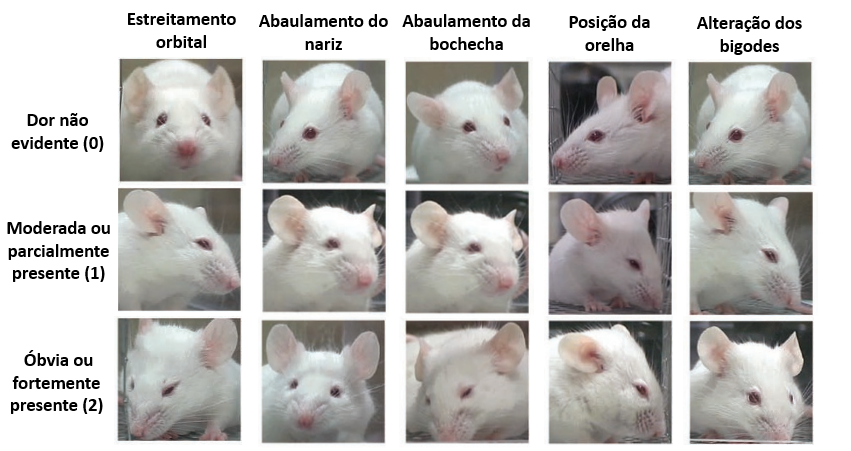
\includegraphics[width=1\linewidth]{figuras/figs_introducao/MGS.png}
	\caption{Indicadores da \acs{MGS} utilizados para a avaliação da dor em camundongos. A figura apresenta cinco unidades de expressões faciais: estreitamento orbital, protrusão nasal, protrusão das bochechas, posição das orelhas e alteração nos bigodes. Para cada característica, são mostrados exemplos representativos correspondentes à três níveis de intensidade: 0 (ausente), 1 (moderado) e 2 (grave). Fonte: Adaptado de \cite{Langford2010}.}
	\label{fig:mgs_indicators}
\end{figure}

A principal contribuição da \acs{MGS} consiste na padronização das análises conduzidas em ambientes experimentais, por meio da definição objetiva das unidades de expressão facial e dos critérios necessários para sua classificação. Entretanto, a avaliação ainda depende da interpretação humana, exigindo avaliadores devidamente treinados para identificar e classificar os indicadores de forma consistente. Em estudos que envolvem grande número de animais ou avaliações seriadas, essa dependência ainda pode representar um desafio operacional.

Diante dessas limitações, técnicas automatizadas baseadas em visão computacional e aprendizado de máquina têm emergido como alternativas promissoras para a avaliação da dor, apresentando potencial para reduzir possíveis vieses humanos e viabilizar avaliações mais ágeis, consistentes e reprodutíveis no contexto da pesquisa com modelos animais \cite{Zamzmi2019}.

Portanto, o presente trabalho propõe o desenvolvimento de um modelo baseado em visão computacional e aprendizado de máquina voltado à identificação automática dos marcadores definidos pela \acs{MGS}, seguido da classificação quanto à presença e intensidade da dor. Além de reduzir a dependência de técnicas manuais de extração de características, o estudo busca ampliar a aplicabilidade das soluções propostas em cenários experimentais próximos de condições reais. Adicionalmente, são investigadas diferentes arquiteturas de redes neurais, analisando o impacto de fatores estruturais — como profundidade das redes, regimes de treinamento e configurações de hiperparâmetros — sobre o desempenho dos modelos.

\section{Motivação}

% SEÇÃO ALTERADA PARA DAR MAIOR IMPORTANCIA AO MEU TRABALHO 
Além das contribuições para a área de visão computacional, ferramentas automatizadas para avaliação da dor apresentam potencial para apoiar médicos-veterinários e pesquisadores durante o monitoramento de animais submetidos a protocolos experimentais. O fornecimento de estimativas objetivas sobre a presença e a intensidade da dor contribuem para decisões relacionadas à administração de analgesia, ao refinamento dos protocolos experimentais e à definição de intervenções clínicas quando necessárias. 

Nesse contexto, a disponibilidade de ferramentas capazes de fornecer avaliações padronizadas da dor também favorece a uniformização das condutas adotadas entre diferentes profissionais e instituições. A redução da variabilidade entre avaliadores contribui para decisões clínicas mais consistentes, além de fortalecer a comparabilidade dos resultados obtidos em estudos e experimentos conduzidos por diferentes grupos de pesquisa.

Por fim, além de automatizar um processo de classificação de imagens, a proposta deste trabalho busca disponibilizar uma ferramenta de apoio à tomada de decisão por médicos-veterinários e pesquisadores, favorecendo a adoção de práticas experimentais mais éticas, padronizadas e reprodutíveis, em conformidade com os princípios contemporâneos de bem-estar animal e refinamento experimental. Dessa forma, a tecnologia proposta deve ser compreendida como um instrumento de complementar — e não substitutivo — do processo de avaliação realizada por profissionais especializados.

\section{Objetivos}

O principal objetivo deste trabalho consiste no desenvolvimento e na avaliação de um sistema baseado em visão computacional e aprendizado de máquina para auxiliar a identificação e a classificação automática da presença e da intensidade da dor em camundongos, utilizando os parâmetros estabelecidos pela \acs{MGS}. Espera-se que a ferramenta desenvolvida contribua para avaliações mais objetivas, padronizadas e reprodutíveis, oferecendo suporte à tomada de decisão por pesquisadores e médicos-veterinários durante o monitoramento de animais utilizados em pesquisas biomédicas. Adicionalmente, o estudo busca investigar diferentes abordagens de classificação baseadas em redes neurais, visando identificar as arquiteturas e configurações mais adequadas para o problema proposto. A partir dessa premissa, o trabalho desdobra-se nos seguintes objetivos específicos:

\begin{enumerate}
	
	\item Realizar um levantamento do estado da arte sobre métodos computacionais aplicados à detecção e classificação de padrões em dados de imagens;
	
	\item Especificar os equipamentos e protocolos empregados na aquisição das imagens utilizadas no estudo;
	
    \item Desenvolver uma ferramenta computacional destinada à extração, organização e gerenciamento das imagens utilizadas na construção da base de dados;
    
    \item Realizar o tratamento das imagens coletadas, adequando-as para as etapas de treinamento e validação dos classificadores;

	\item Implementar os modelos neurais responsáveis pelas classificação dos padrões faciais associados à dor, de acordo com a \acs{MGS};
	
	\item Treinar e avaliar os modelos implementados, utilizando métricas adequadas de desempenho;
	
	\item Realizar uma análise comparativa entre os modelos investigados, buscando identificar as arquiteturas mais otimizadas para o problema proposto;
	
	\item Investigar o impacto de diferentes configurações de hiperparâmetros e estratégias de treinamento sobre o desempenho dos modelos.
	
	%\item Analisar as implicações práticas da utilização de sistemas automatizados para detecção de dor em contextos experimentais e veterinários.
    
\end{enumerate}

\section{Hipótese}

A hipótese central deste estudo é que modelos neurais aplicados à visão computacional sejam capazes de identificar automaticamente os indicadores estabelecidos pela \acs{MGS} em imagens das regiões faciais de camundongos, possibilitando a detecção e a quantificação da dor.

Parte-se do pressuposto de que a extração automatizada e padronizada de características visuais possibilite a identificação de nuances associadas aos indicadores da \acs{MGS}, inclusive padrões sutis que dificilmente seriam detectados por observadores não especializados.

\section{Revisão do Estado da Arte}

O problema da identificação e quantificação da dor não é recente, porém ainda apresenta desafios e limitações significativos, os quais motivam o desenvolvimento de novas técnicas e abordagens para sua análise. Nesse contexto, os avanços recentes em visão computacional e aprendizado de máquina têm impulsionado diferentes estudos voltados à identificação e classificação automática de sinais associados à dor em diferentes espécies animais.

% CITAÇÃO AO TUTTLE ALTERADA PARA DIFERENCIAR MELHOR DESTA PESQUISA
O estudo desenvolvido por \cite{Tuttle2018DNNPain} representa um dos primeiros trabalhos a investigar a aplicação de aprendizado profundo para automatizar a \acs{MGS}. Os autores propuseram um sistema baseado na arquitetura convolucional InceptionV3, treinado com aproximadamente 5.700 imagens previamente rotuladas por especialistas, cujo objetivo consistiu em substituir a pontuação manual realizada por avaliadores humanos. O modelo realizou uma classificação binária entre presença e ausência de dor, alcançando aproximadamente 94\% de acurácia e elevada correlação com as avaliações humanas.

Embora esse estudo tenha demonstrado a viabilidade da automatização da MGS, sua investigação concentrou-se na validação de uma única arquitetura convolucional e em um cenário específico de classificação binária. Aspectos relacionados ao impacto de diferentes arquiteturas neurais, estratégias de treinamento, configurações de hiperparâmetros e modelos baseados em mecanismos de atenção não foram explorados. Em contraste, o presente trabalho adota uma perspectiva mais ampla ao investigar comparativamente diferentes modelos de aprendizado profundo. Dessa forma, além de propor uma solução computacional, esta pesquisa busca compreender quais abordagens apresentam maior potencial para o problema proposto.

Outra contribuição relevante foi apresentada por \cite{Wotton2020}, que desenvolveram um sistema automatizado de fenotipagem comportamental aplicado ao teste da formalina em camundongos. O estudo teve como objetivo automatizar a identificação de comportamentos nociceptivos — como lamber, morder e elevar a pata — sem depender de observação humana contínua. Diferentemente da abordagem baseada na \acs{MGS}, o trabalho concentrou-se em padrões comportamentais corporais, e não exclusivamente em expressões faciais.

A metodologia proposta foi estruturada em três etapas principais. Inicialmente, foi feita a detecção de pontos-chave corporais por meio do \textit{DeepLabCut}, ferramenta baseada em \acsp{CNN} com arquitetura \textit{ResNet}-50. Em seguida, foram extraídas características espaço-temporais utilizando distâncias euclidianas e ângulos entre pontos anatômicos ao longo das sequências temporais. Por fim, os comportamentos nociceptivos foram classificados utilizando o algoritmo \textit{GentleBoost}, baseado em conjuntos de árvores de decisão. O sistema alcançou concordância de 98\% em relação às avaliações humanas.

Abordagens semelhantes também têm sido aplicadas em outras espécies animais. No contexto veterinário, \cite{lencioni2021} investigaram a detecção automática de dor em equinos por meio da análise de expressões faciais indicadas pela \textit{Grimace Scale}. O sistema desenvolvido utilizou \acsp{CNN} independentes para analisar diferentes regiões da face — incluindo orelhas, olhos e boca/narinas — cujas saídas foram posteriormente integradas em um classificador global responsável pela decisão final. Os resultados indicaram que o modelo dedicado à análise das orelhas apresentou o melhor desempenho individual, alcançando acurácia de 90,3\%. Já os modelos associados às regiões dos olhos e boca/narinas obtiveram acurácias de 65,5\% e 74,5\%, respectivamente. Na classificação global, o sistema atingiu acurácia de 75,8\%. Contudo, quando a tarefa foi simplificada para classificação binária entre presença e ausência de dor, o valor de acurácia subiu para 88,3\%.

Além das aplicações veterinárias, métodos automatizados de detecção da dor também vêm sendo investigados no contexto humano. O trabalho descrito por \cite{karamitsos2021} propõe uma abordagem baseada em \acsp{CNN} para monitoramento automático da dor em pacientes clínicos por meio de expressões faciais, visando aplicações em sistemas hospitalares de monitoramento contínuo. O estudo utilizou a base de dados \textit{UNBC-McMaster Shoulder Pain Expression Archive}, amplamente empregada na literatura para tarefas de reconhecimento de expressões faciais associadas à dor. Após as etapas de pré-processamento, as imagens foram utilizadas no treinamento de uma versão adaptada da arquitetura \textit{\acs{VGG}16} para a indicação da presença ou ausência de dor.

Os resultados deste estudo demonstraram acurácia de 92,5\% e \textit{recall} de 86,96\% no conjunto de teste, superando abordagens previamente reportadas na literatura, incluindo modelos híbridos e arquiteturas recorrentes. Apesar do desempenho satisfatório, os autores destacaram limitações relacionadas ao desbalanceamento das classes e à necessidade de ampliar a diversidade do conjunto de treinamento, com enfoque no desenvolvimento de estratégias futuras voltadas à redução de falsos positivos.

É importante destacar que os estudos supracitados compartilham uma característica comum: o uso predominante de modelos neurais convolucionais. Os quais foram especificamente projetados para processamento de dados com estrutura espacial, -- como imagens -- e consolidaram-se na literatura devido a capacidade de realizar extração automática de características relevantes, além da elevada eficiência observada em tarefas de visão computacional. Entretanto, apesar dos avanços proporcionados pelas \acsp{CNN}, tais arquiteturas apresentam limitações relacionadas à modelagem de dependências globais na imagem, uma vez que operam predominantemente sobre padrões locais extraídos por convoluções sucessivas. Nesse cenário, arquiteturas baseadas em mecanismos de atenção, como os \textit{Vision Transformers} (\acsp{VIT}), surgem como alternativas promissoras para aprendizado de representações visuais mais abrangentes.

O estudo desenvolvido por \cite{barman2024} investigou o uso de arquiteturas \acs{VIT} para detecção de doenças em folhas de tomate, realizando uma comparação direta com a arquitetura \textit{InceptionV3}. Adicionalmente, os autores propuseram a implementação de um aplicativo para dispositivos \textit{Android} voltado à detecção em tempo real por meio de imagens capturadas por \textit{smartphones}.

Para os experimentos, foi utilizado um subconjunto do \textit{PlantVillage Dataset}, contendo 10.010 imagens distribuídas entre folhas saudáveis e nove classes distintas de doenças do tomateiro. Após as etapas de pré-processamento e normalização, ambos os modelos foram treinados durante 30 épocas. Os resultados demonstraram desempenho superior do modelo \acs{VIT} em praticamente todas as métricas avaliadas, alcançando acurácia de 97,34\% no treinamento e 95,76\% na validação, enquanto a InceptionV3 atingiu 94,8\% e 94,02\%, respectivamente.

No contexto específico da detecção de dor, o estudo conduzido por \cite{fiorentini2022} descreve uma abordagem baseada em \textit{Vision Transformers} (\acs{VIT}) e \textit{Video Vision Transformers} (\acs{ViVIT}), aplicados para a indicação da presença ou ausência da dor. O treinamento foi conduzido utilizando o conjunto \textit{UNBC-McMaster Shoulder Pain}, cujas amostras são rotuladas com base na escala \acs{PSPI} (\textit{Prkachin and Solomon Pain Intensity}).

Os autores empregaram técnicas de registro facial tridimensional utilizando as ferramentas \textit{PRNet} e \textit{Face3D}, permitindo padronização frontal das imagens e maior consistência entre os indivíduos e os respectivos quadros do vídeo. Enquanto o \acs{VIT} foi utilizado para análise de imagens estáticas, o \acs{ViVIT} foi empregado para processamento das sequências dos quadros, incorporando simultaneamente informações espaciais e temporais. Os resultados demonstraram que os modelos \acs{VIT}-1 e \acs{ViVIT}-1 alcançaram \textit{F1-score} médio de 0,55, superando abordagens baseadas em \acsp{CNN} -- como o modelo \textit{Pain Facial Deep Learning} (\acs{PFDL}) -- o qual apresentou \textit{F1-score} de 0,47. Além do desempenho quantitativo, o estudo destacou a interpretabilidade proporcionada pelos mapas de atenção gerados pelos modelos, os quais evidenciaram foco em regiões faciais anatomicamente relevantes para a identificação da dor.

% TABELA ANÁLOGA À APRESENTAÇÃO
Os estudos apresentados evidenciam uma grande diversidade de cenários experimentais, espécies investigadas, arquiteturas empregadas e objetivos específicos, dificultando uma comparação direta entre as abordagens propostas. Com o intuito de sintetizar essas diferenças e destacar as principais características de cada estudo, a Tabela \ref{tab:estado_arte} apresenta um resumo comparativo dos trabalhos discutidos nesta seção.

\begin{table}[h]
	\centering
	\footnotesize
	\caption{Comparação dos trabalhos correlatos relacionados ao aprendizado profundo e visão computacional.}
	\label{tab:estado_arte}
	
	\renewcommand{\arraystretch}{1.3}
	
	\begin{tabular}{l|c|c|c}
		
		\toprule
		
		\textbf{Referência} &
		\makecell{\textbf{Modelo}\\ \textbf{Experimental}} &
		\makecell{\textbf{Objetivo}\\ \textbf{Central}} &
		\textbf{Resultados} \\
		
		\midrule
		
		\makecell{Tuttle et al.\\(2018)}&
		Camundongos&
		\makecell{Automatizar a MGS para\\classificação da presença de dor.}&
		Acc. 94\%
		\\
		
		\midrule
		
		\makecell{Wotton et al.\\(2020)}&
		Camundongos&
		\makecell{Classificar comportamentos nociceptivos\\utilizando visão computacional.}&
		Acc. 98\%
		\\
		
		\midrule
		
		\makecell{Lencioni et al.\\(2021)}&
		Equinos&
		\makecell{Detectar dor em equinos pela\\HGS utilizando CNNs.}&
		Acc. 75,8\%
		\\
		
		\midrule
		
		\makecell{Karamitsos et al.\\(2021)}&
		Humanos&
		\makecell{Reconhecimento automático\\da dor por expressões faciais.}&
		\makecell{Acc. 92,5\%\\Recall 86,9\%}
		\\
		
		\midrule
		
		\makecell{Barman et al.\\(2024)}&
		\makecell{Folhas de\\Tomate}&
		\makecell{Avaliação da ViT para\\reconhecimento automático da dor.}&
		F1-score 0,55
		\\
		
		\midrule
		
		\makecell{Fiorentini et al.\\(2022)}&
		Humanos&
		\makecell{Avaliação da ViT para\\reconhecimento automático da dor.}&
		F1-score 0,55
		\\
		
		\bottomrule
		
	\end{tabular}
	
\end{table}

A compreensão das diferenças entre \acsp{CNN} e \acsp{VIT} torna-se fundamental para contextualizar os avanços recentes em classificação de imagens. O estudo descrito por \cite{mauricio2023} apresenta uma revisão sistemática da literatura, com foco na comparação entre ambas as arquiteturas para tarefas de classificação. Considerando a consolidação das \acsp{CNN} como abordagem predominante e o surgimento recente dos \acsp{VIT}, os autores analisam as condições em que cada arquitetura apresenta melhor desempenho, além de discutir suas vantagens, limitações e aplicações práticas.

Os autores observaram que o desempenho relativo entre \acsp{CNN} e \acsp{VIT} depende fortemente das características do conjunto de dados e do cenário de aplicação. Arquiteturas baseadas em atenção demonstraram vantagens na modelagem de relações globais das imagens, enquanto as \acsp{CNN} apresentaram maior robustez para tarefas gerais de menor complexidade. Adicionalmente, arquiteturas híbridas — combinando convoluções e mecanismos de atenção — apresentaram resultados promissores ao explorar simultaneamente características locais e globais das imagens. A revisão conclui que não existe uma arquitetura universalmente superior, mas sim, diferentes contextos nos quais cada abordagem pode se tornar mais vantajosa.

\section{Contribuições}

% LIGAÇÃO COM O CONTEXTO HUMANO
As ferramentas computacionais capazes de apoiar a avaliação da dor contribuem diretamente para a condução de pesquisas biomédicas, uma vez que alterações fisiológicas e comportamentais decorrentes da dor podem comprometer a confiabilidade dos dados experimentais e introduzir variáveis de confusão capazes de influenciar a interpretação dos resultados. Ao fornecer avaliações mais objetivas, padronizadas e reprodutíveis, esses sistemas favorecem decisões mais consistentes relacionadas ao manejo dos animais e ao refinamento dos protocolos experimentais. Como consequência, espera-se que os achados desta pesquisa contribua para a obtenção de resultados pré-clínicos mais robustos e confiáveis, servindo inclusive como base para o processo de translação do conhecimento científico obtido em modelos animais para aplicações na medicina humana.

Do ponto de vista da Computação, esta pesquisa amplia o entendimento sobre a aplicação de diferentes paradigmas de aprendizado profundo no contexto da avaliação automatizada da dor. A investigação comparativa entre arquiteturas convolucionais pertencentes às famílias \textit{ResNet}, \textit{DenseNet} e \textit{MobileNet}, associada à inclusão de um modelo baseado em mecanismos de autoatenção \acs{VIT}, permitiu analisar como diferentes estratégias de extração de características, conectividade e representação espacial influenciam o desempenho da tarefa de classificação. Dessa forma, a pesquisa contribui não apenas com a proposição de um modelo computacional, mas também com uma análise experimental sobre o comportamento dessas arquiteturas em um problema biomédico específico.

Adicionalmente, esta pesquisa também apresenta uma contribuição de caráter prático ao investigar arquiteturas neurais com diferentes níveis de complexidade computacional, incluindo modelos leves, como a \textit{MobileNet} e variantes menos profundas da \textit{ResNet}, bem como adaptações estruturais da \textit{DenseNet}. Essa abordagem demonstra que é possível obter modelos com bom desempenho preditivo sem necessariamente recorrer às arquiteturas mais complexas, favorecendo o desenvolvimento de soluções mais acessíveis, escaláveis e potencialmente aplicáveis em diferentes ambientes de pesquisa e monitoramento experimental.

Além das contribuições relacionadas ao desenvolvimento e à avaliação dos modelos classificadores, esta pesquisa disponibiliza publicamente toda a infraestrutura computacional desenvolvida, incluindo a ferramenta para geração e organização da base de dados, o conjunto de imagens utilizado nos experimentos e a implementação completa dos modelos avaliados. A disponibilização desses recursos favorece a transparência científica, a reprodutibilidade dos experimentos e o reaproveitamento da infraestrutura proposta por outros grupos de pesquisa, contribuindo para o avanço de estudos envolvendo visão computacional aplicada à avaliação da dor em modelos animais.

\section{Organização da Dissertação}

O presente trabalho encontra-se dividido em 5 capítulos organizados da seguinte forma:

\begin{itemize}
	
	\item O Capítulo 1 introduz o contexto geral da pesquisa, apresentando a problemática relacionada à avaliação de dor em camundongos, bem como sua relevância para o bem-estar animal, a ética científica e a confiabilidade experimental. Em seguida, são discutidas as motivações que fundamentam o desenvolvimento deste estudo, os objetivos gerais e específicos, as hipóteses levantadas e as principais contribuições propostas. O capítulo também apresenta uma revisão da literatura relacionada ao estado da arte, abordando trabalhos mais recentes e relevantes nas áreas de visão computacional, aprendizado profundo e avaliação automatizada de dor.
	
	\item O Capítulo 2 apresenta os fundamentos teóricos que sustentam o desenvolvimento da pesquisa, fornecendo a base conceitual necessária para a compreensão das técnicas, arquiteturas e ferramentas empregadas ao longo do trabalho. Inicialmente, são discutidos os princípios fundamentais do Processamento Digital de Imagens e do Aprendizado de Máquina, que constituem a base metodológica utilizada na construção dos experimentos.
	
	Na sequência, o capítulo aprofunda-se nos conceitos relacionados às Redes Neurais Convolucionais e aos modelos baseados em \textit{Transformers} aplicados à Visão Computacional, destacando seus mecanismos de funcionamento, estratégias de aprendizado e relevância para tarefas de classificação de imagens. Também são abordados conceitos complementares, como \textit{Transfer Learning}, técnicas de regularização e métodos de avaliação de desempenho.
	
	\item O Capítulo 3 descreve a metodologia adotada para a condução da etapa experimental, detalhando os procedimentos técnicos empregados na aquisição, organização, processamento e análise dos dados, de modo a garantir a reprodutibilidade científica dos experimentos realizados.
	
	Inicialmente, é apresentado o protocolo experimental utilizado para aquisição e organização da base de dados, abrangendo as etapas de coleta, preparação e estruturação das amostras utilizadas no treinamento dos modelos. Em seguida, são detalhadas as estratégias de aprendizado de máquina adotadas ao longo da pesquisa, incluindo a seleção das arquiteturas investigadas, os critérios utilizados para definição das configurações de treinamento, os métodos de otimização empregados e as métricas utilizadas para avaliação de desempenho dos modelos.
	
	\item O Capítulo 4 apresenta os experimentos conduzidos ao longo da pesquisa, bem como os resultados obtidos com cada arquitetura investigada. Inicialmente, são descritos os experimentos preliminares realizados para validação dos modelos e verificação da estabilidade do processo de treinamento. Em seguida, são apresentados os experimentos principais, incluindo análises comparativas entre diferentes arquiteturas e configurações de treinamento.
	
	O capítulo também  realizada uma análise crítica dos resultados obtidos, destacando as vantagens, limitações e implicações práticas das abordagens investigadas no contexto da avaliação automatizada de dor em camundongos;
	
	\item O Capítulo 5 apresenta as considerações finais da pesquisa, sintetizando os principais resultados obtidos e discutindo suas implicações científicas e práticas. O capítulo retoma os objetivos e hipóteses inicialmente estabelecidos, analisando em que medida os experimentos conduzidos foram capazes de responder às questões propostas. 
	
	Por fim, são discutidas as limitações do trabalho e apresentadas perspectivas para trabalhos futuros, incluindo possíveis melhorias metodológicas, expansão do conjunto de dados e investigação de arquiteturas emergentes voltadas para aplicações em ambientes reais de pesquisa biomédica.
	
\end{itemize}


% ----------------------------------------------------------
% Fundamentação
% ----------------------------------------------------------
\chapter[Fundamentação Teórica]{Fundamentação Teórica}

No presente trabalho, os modelos baseados em estratégias convolucionais e nos mecanismos de atenção, compõem as principais abordagens para problemas de classificação aplicados à detecção de dor. A construção de classificadores eficientes nesse contexto requer a compreensão de diferentes etapas fundamentais, que estruturam todo o processo de modelagem.

Entre essas etapas, destacam-se: (i) o pré-processamento dos dados, responsável por adequar o conjunto de imagens aos requisitos de entrada dos modelos; (ii) a definição da arquitetura da rede, orientada pelas características do problema e pela complexidade dos padrões visuais a serem aprendidos; e (iii) a validação dos resultados, realizada por meio de métricas específicas que avaliam o desempenho e a capacidade de generalização dos modelos. Cada uma dessas etapas desempenha um papel essencial para a confiabilidade do sistema, sendo discutidas ao longo desta seção.

\section{Processamento Digital de Imagens - \acs{PDI}}

O processamento digital de imagens (\acs{PDI}) é um campo da ciência da computação voltado ao processamento, à análise e à interpretação de imagens digitais. Suas técnicas abrangem desde a aquisição e o pré-processamento dos dados visuais até a extração de características relevantes, fornecendo subsídios para tarefas como reconhecimento de padrões, classificação e suporte à tomada de decisão.

Uma imagem digital pode ser entendida como uma representação discreta de dados, composta por informações espaciais — relacionadas à sua estrutura geométrica — e por atributos de intensidade, como cor, contraste e luminosidade. Devido à sua capacidade de representar informações complexas de forma visual e intuitiva, imagens digitais tornaram-se fundamentais em diversas áreas, como ciência, medicina, segurança e tecnologia.

Após a aquisição, uma imagem digital pode ser submetida a diferentes etapas de processamento com o objetivo de realçar informações relevantes e reduzir fatores que possam comprometer sua análise. Entre as operações mais comuns estão a normalização de intensidades, o realce de contraste, a remoção de ruído, a segmentação de regiões de interesse e a extração de características visuais, como formas, texturas e contornos. Em conjunto, essas técnicas contribuem para a obtenção de representações mais informativas e consistentes dos dados visuais, favorecendo o desempenho de sistemas de visão computacional em tarefas como classificação, detecção de objetos e reconhecimento de padrões.

De acordo com a literatura, o processamento das imagens pode ser subdividido em diferentes categorias, as quais podem ser aplicadas de modo independente, de acordo com contexto:

\begin{itemize}

    \item \textbf{Aquisição da imagem:} etapa inicial, na qual a imagem é capturada por sensores, câmeras digitais ou outros dispositivos. O resultado é uma representação numérica matricial, que pode conter ruídos ou distorções;
    
    \item \textbf{Pré-processamento:} responsável por melhorar a qualidade da imagem e reduzir variações indesejadas. Inclui operações como redimensionamento, normalização dos valores de \textit{pixels}, filtragem de ruído (por exemplo, filtros de média ou Gaussiano) e ajuste de contraste;

    \item \textbf{Segmentação:} consiste na divisão da imagem em regiões significativas, facilitando a identificação de áreas de interesse. Técnicas comuns incluem limiarização, detecção de bordas e agrupamento de \textit{pixels};

    \item \textbf{Extração de características:} etapa voltada à obtenção de atributos relevantes, como formas, texturas e padrões, que servirão como entrada para algoritmos de classificação;
    
    \item \textbf{Pós-processamento:} etapa destinada ao refinamento dos resultados provenientes das operações anteriores, podendo incluir ajustes visuais ou realces adicionais;

    \item \textbf{Classificação ou Reconhecimento:} envolve a aplicação de algoritmos capazes de interpretar os padrões extraídos e atribuir rótulos às amostras.

\end{itemize}

No contexto deste trabalho, o \acs{PDI} é essencial na preparação das imagens para os modelos de aprendizado de máquina, que geralmente exigem dados de entrada padronizados em termos de dimensão, estrutura e escala de valores. O exemplo apresentado na Figura \ref{fig:preprocessing} ilustra parte deste processo. 

\begin{figure}[h]
    \centering
    \includegraphics[width=0.8\linewidth]{pre_processing.png}
    \caption{Exemplo de operações aplicadas a uma imagem destinada à entrada de um modelo classificador. O redimensionamento e a conversão para escala de cinza reduzem significativamente a quantidade dos dados de entrada e, consequentemente, o custo computacional associado às etapas. A normalização, por sua vez, reescala os valores de intensidade dos pixels para o intervalo entre 0 e 1, padronizando a faixa de valores da imagem e favorecendo a estabilidade numérica durante o treinamento do modelo. Fonte: o autor.}
    \label{fig:preprocessing}
\end{figure}

Por fim, enquanto o \acs{PDI} se concentra na melhoria e preparação das imagens, a visão computacional busca atribuir significado a essas informações, por meio de modelos de inferência e aprendizado. Para aprofundamento no tema, recomenda-se a obra \textit{Digital Image Processing} \cite{gonzalez2010}.

\section{Aprendizado de Máquina}

O aprendizado de máquina (\textit{machine learning} – \acs{ML}) é uma subárea da inteligência artificial voltada ao desenvolvimento de sistemas capazes de aprender padrões a partir de dados e realizar previsões ou decisões de forma automatizada. Em vez de serem explicitamente programados para cada tarefa, esses sistemas utilizam exemplos para inferir regras e generalizar o conhecimento adquirido. As abordagens de aprendizado de máquina são tradicionalmente classificadas em três categorias principais:

\begin{itemize}
    \item \textbf{Aprendizado supervisionado:} uma das abordagens mais comuns de \acs{ML}, onde um modelo é treinado com base em um conjunto de dados previamente conhecidos e rotulados. Isso significa que o algoritmo recebe pares de entrada e saída conhecidos e aprende a mapear essas entradas para as saídas corretas. A ideia principal é ajustar o modelo para que ele possa generalizar e fazer previsões precisas para novos conjuntos de dados;
    
    \item \textbf{Aprendizado não supervisionado:} uma abordagem comum para lidar com dados que não possuem rótulos definidos. Neste caso, a ideia do algoritmo é explorar a estrutura subjacente dos dados e identificar padrões ocultos, agrupando os dados com base em características similares;
	
    \item \textbf{Aprendizado por reforço:} uma abordagem baseada no \textit{feedback} recebido por meio das interações de um agente com um determinado ambiente ou situação. A cada ação tomada, o agente recebe uma recompensa ou uma penalidade com base no impacto de suas decisões. O objetivo é maximizar as recompensas acumuladas ao longo do tempo, ajustando o comportamento do agente para melhorar a performance. 
\end{itemize}

No contexto do aprendizado não-supervisionado, uma das técnicas mais representativas é o agrupamento de dados (\textit{clustering}), cujo objetivo é particionar um conjunto de dados em grupos formados com base na semelhança entre as amostras, sem a utilização de rótulos previamente definidos. Nesse tipo de abordagem, os algoritmos buscam organizar os dados de forma coesa, de modo que elementos pertencentes a um mesmo grupo apresentem alta similaridade entre si, enquanto elementos de grupos distintos sejam significativamente diferentes.

Para viabilizar esse processo, o conceito de similaridade torna-se central, sendo definido como uma medida que quantifica o grau de proximidade entre amostras com base em suas representações numéricas. Essa proximidade pode ser avaliada por diferentes métricas, como distância Euclidiana, distância de \textit{Manhattan} ou similaridade do cosseno. Algoritmos como \textit{K-means}, \textit{DBSCAN} e \textit{Expectation Maximization} utilizam essas medidas para estruturar os dados em grupos, revelando padrões latentes sem qualquer conhecimento prévio das classes reais \cite{jain1999}.

Embora os resultados do agrupamento possam ser interpretados como uma forma de organização ou até mesmo de classificação implícita dos dados, é importante destacar que essa associação é construída exclusivamente a partir de critérios matemáticos de similaridade, e não de rótulos previamente conhecidos. Em contraste, o aprendizado supervisionado exige um conjunto de dados rotulado, no qual cada amostra possui uma saída conhecida (\textit{ground truth}). Nesse cenário, o objetivo do modelo é aprender uma função que relacione corretamente as entradas às suas respectivas saídas, ajustando seus parâmetros de forma iterativa para minimizar o erro de predição. O exemplo apresentado pela Figura \ref{fig:Fig_aprendizado}, deixa clara a distinção das abordagens supervisionada e não-supervisionada,

\begin{figure}[h]
    \centering
    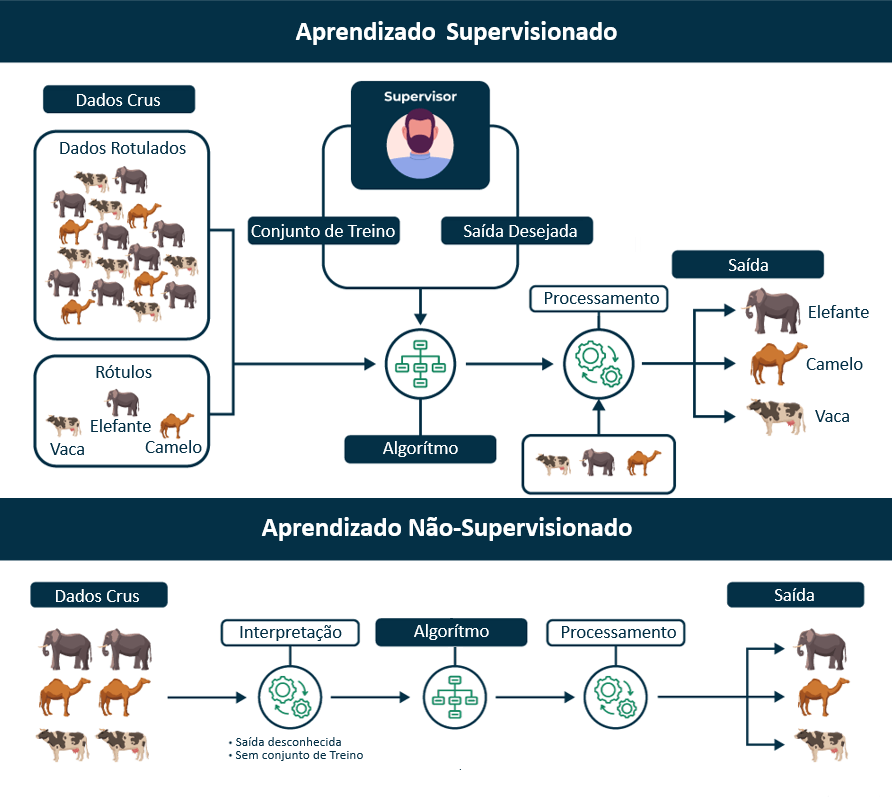
\includegraphics[width=.95\linewidth]{learning_comparison.png}
    \caption{Comparativo entre as abordagens de aprendizado de máquina. Na abordagem não-supervisionada os animais são agrupados automaticamente conforme a similaridade de suas características visuais. Já na abordagem supervisionada, destaca-se a presença de um agente supervisor, responsável por fornecer ao sistema um gabarito como base para o reconhecimento de padrões entre as associações explícitas de entrada e saída. Fonte: Adaptado de \cite{moritz2024}.}
    \label{fig:Fig_aprendizado}
\end{figure}

A literatura apresenta uma ampla variedade de técnicas supervisionadas para problemas de classificação e regressão. Entre os métodos clássicos, destacam-se: Regressão Logística, Árvores de Decisão e \textit{Support Vector Machines} (\acs{SVM}). Os detalhes técnicos dos métodos citados previamente podem ser consultados no capítulo 2 do livro \textit{Machine Learning for Brain Disorders} \cite{faouzi2023} ou, de forma mais abrangente no livro \textit{The Elements of Statistical Learning} \cite{hastie2009}. 

Entre os modelos mais avançados, destacam-se principalmente as técnicas baseadas em redes neurais, cujo principal diferencial está na automatização do processo de extração de características e reajuste de pesos (via \textit{backpropagation}), tornando-se especialmente úteis para a análise e classificação de dados complexos. É importante destacar que, as técnicas supervisionadas baseadas em redes neurais exigem um treinamento prévio com uma base robusta, a fim de promover o ajuste de pesos e, consequentemente a generalização.


\section{Aprendizado Baseado em Redes Neurais}

As Redes Neurais Artificiais (\acsp{RNA}) constituem uma das principais abordagens no campo do aprendizado de máquina, especialmente quando se busca modelar relações complexas em dados de alta dimensionalidade. Inspiradas no funcionamento do cérebro humano, essas redes são compostas por unidades de processamento denominadas neurônios artificiais, organizadas em camadas interconectadas, conforme ilustrado na Figura \ref{fig:ann_architecture}. Um dos principais diferenciais das \acsp{RNA} é sua capacidade em aprender representações ocultas e abstratas de forma automática, o que as torna altamente eficazes em tarefas como classificação, regressão e tomada de decisão.

\begin{figure}[h]
    \centering
    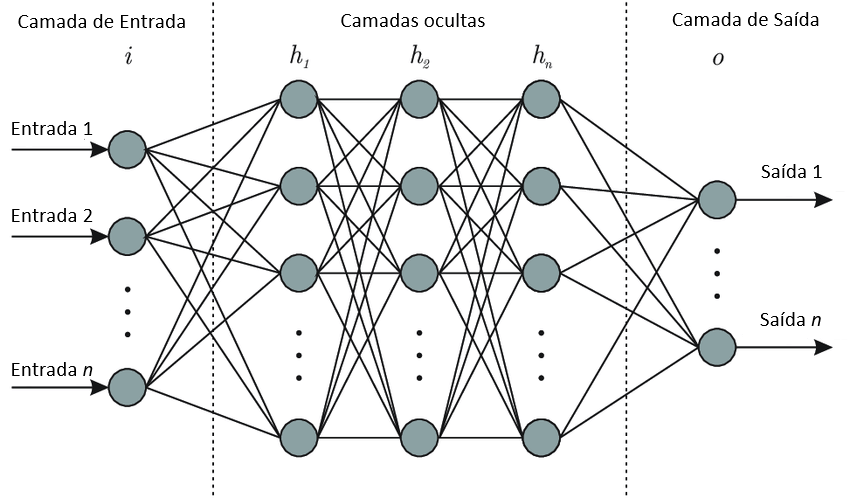
\includegraphics[width=.8\linewidth]{ann_architecture.png}
    \caption{Arquiteura de uma \acs{RNA}. Fonte: Adaptado de \cite{Alqahtani2020}.} 
    \caption*{\small A camada de entrada é responsável exclusivamente pelo transporte de dados para as camadas ocultas, as quais são responsáveis por realizar transformações mais críticas que permitem a extração de características dos dados pela rede; A camada de saída é responsável por fornecer a previsão ou o resultado do modelo.}
    
    \label{fig:ann_architecture}
\end{figure}

Os neurônios artificiais constituem as unidades básicas de processamento dessas redes. Sua função é receber entradas, processá-las por meio de operações matemáticas e produzir uma saída que será propagada para os neurônios da camada seguinte. Embora o funcionamento de um único neurônio seja relativamente simples, a organização desses elementos em múltiplas camadas interconectadas permite a modelagem de relações altamente complexas entre os dados.

À medida que a informação percorre as camadas mais profundas, os neurônios passam a atuar de forma cooperativa, identificando padrões em diferentes níveis de abstração. Em aplicações envolvendo imagens, por exemplo, as camadas iniciais tendem a aprender padrões mais simples, como bordas e texturas, enquanto camadas intermediárias e profundas capturam estruturas mais complexas, como formas, objetos ou até mesmo expressões faciais completas.

Um elemento central no funcionamento das \acsp{RNA} é o peso sináptico, que corresponde ao valor numérico associado a cada conexão entre neurônios. Esses pesos determinam a importância relativa de cada entrada no processo de decisão do neurônio e constituem os principais parâmetros ajustáveis do modelo. Durante o treinamento, os valores são atualizados iterativamente por meio do algoritmo de retropropagação (\textit{backpropagation}), no qual o cálculo dos gradientes da função de perda (loss function) é utilizado para o ajuste dos pesos definidos nas camadas anteriores, levando à minimização dos erros de predição. Para um aprofundamento técnico, recomenda-se a literatura \textit{State-of-the-art in artificial neural network applications: A survey} \cite{abiodun2018}.

As redes neurais artificiais podem ser estruturadas de acordo com os requisitos específicos de cada aplicação visando, a melhorara do desempenho, redução do custo computacional ou a adaptação do modelo a diferentes tipos de dados. Nesse contexto, o termo 'arquitetura de rede' refere-se à forma como os neurônios são organizados e conectados, incluindo aspectos como número de camadas, funções de ativação, fluxo de dados e estratégias de regularização e treinamento.

Dentre as arquiteturas clássicas, destaca-se o \textit{Multilayer Perceptron} (\acs{MLP}), considerado uma extensão do \textit{perceptron} simples. A \acs{MLP} é composta por camadas densamente conectadas (\textit{fully connected}), nas quais cada neurônio de uma camada está conectado a todos os neurônios da camada seguinte. Além disso, trata-se de uma arquitetura do tipo \textit{feedforward}, na qual a informação flui em uma única direção, da entrada até a saída, sem conexões cíclicas.

Essa arquitetura é capaz de aprender representações não lineares dos dados, sendo particularmente eficaz em tarefas envolvendo dados tabulares ou vetoriais. No entanto, seu desempenho tende a ser limitado quando aplicada a dados com estrutura espacial complexa, como imagens, uma vez que não preserva relações locais entre os elementos de entrada. Nesse contexto, as \acsp{MLP} desempenham um papel fundamental como base para o desenvolvimento de arquiteturas mais profundas, como as Redes Neurais Densas (\acsp{DNN}), conforme ilustrado na Figura \ref{fig:dnn_vs_mlp}.

\begin{figure}[h]
	\centering
	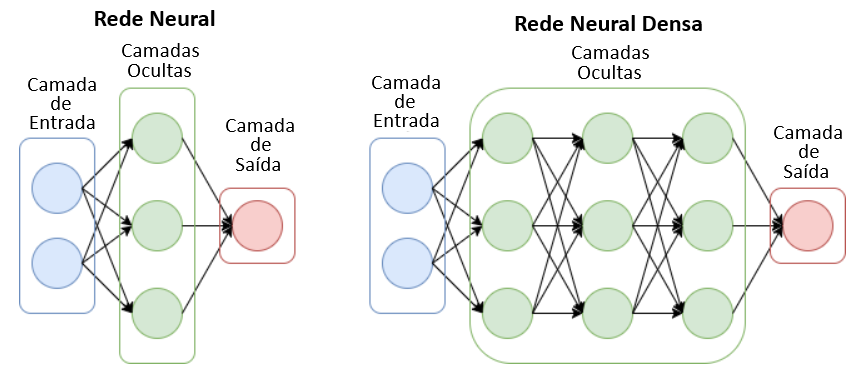
\includegraphics[width=.9\linewidth]{dnn_vs_mlp.png}
	\caption{Comparativo estrutural entre \acs{MLP} e \acs{DNN}. As redes densas mantêm a estrutura das \acsp{MLP}, porém ampliam sua profundidade por meio da adição de múltiplas camadas ocultas, o que aumenta significativamente sua capacidade de representação e abstração. Fonte: Adaptado de \cite{Wehbe2020}.}
	\label{fig:dnn_vs_mlp}
\end{figure}

A evolução das \acsp{MLP} para arquiteturas mais profundas evidencia o potencial das redes neurais em lidar com problemas cada vez mais complexos. Embora inicialmente desenvolvidas para dados vetoriais, as \acsp{DNN} demonstraram capacidade de adaptação a diferentes domínios, incluindo dados de alta dimensionalidade, como imagens, desde que adequadamente representados.

Tal processo evolutivo destaca a flexibilidade das redes neurais artificiais, cuja estrutura pode ser ajustada conforme a natureza do problema e o tipo de dado disponível. Essa característica foi essencial viabilizar o surgimento de arquiteturas mais especializadas, como as Redes Neurais Convolucionais (\acsp{CNN}) e os \textit{Vision Transformers} (\acsp{VIT}) no campo de visão computacional.

\section{Visão Computacional}

A visão computacional é um campo da inteligência artificial dedicado ao processamento e à interpretação de informações visuais provenientes do mundo real. Seu objetivo central é permitir que sistemas computacionais adquiram, analisem e interpretem imagens ou vídeos, executando tarefas que tradicionalmente dependiam da interpretação manual. Uma aplicação em visão computacional geralmente envolve um conjunto de etapas fundamentais, responsáveis por converter informações visuais em representações interpretáveis, sendo:
\begin{itemize}

    \item \textbf{Aquisição da imagem:} corresponde à captura da imagem ou vídeo por meio de dispositivos como câmeras digitais, microscópios ou sensores, responsáveis por digitalizar a cena e convertê-la em uma matriz de \textit{pixels} processável;
    
    \item \textbf{Pré-processamento:} etapa em que são aplicadas técnicas de processamento digital de imagens (\acs{PDI}), como filtragem, redimensionamento, normalização e realce de contraste, com o objetivo de melhorar a qualidade da imagem ou adequá-la às exigências do modelo;
    
    \item \textbf{Extração de características:} consiste na identificação de padrões relevantes para a análise, como bordas, contornos, texturas e formas geométricas;
    
    \item \textbf{Análise, classificação e interpretação:} etapa final, na qual técnicas de aprendizado de máquina são empregadas para classificar, segmentar ou reconhecer padrões visuais a partir das características extraídas. 
    
\end{itemize} 

O avanço neste setor está fortemente associada à evolução das redes neurais convolucionais, especialmente no que se refere à automatização da extração de características relevantes nos dados, possibilitando o desenvolvimento de modelos capazes reduzir significativamente a dependência da interpretação humana. Para um aprofundamento teórico, recomenda-se a obra \textit{Computer Vision: Algorithms and Applications} \cite{szeliski2010}.

Nesse contexto, as \acsp{CNN} utilizam filtros convolucionais para extrair automaticamente representações hierárquicas e progressivamente mais abstratas das imagens. Mais recentemente, arquiteturas baseadas nos mecanismos de atenção -- como os \acsp{VIT} -- passaram a ganhar destaque. Inspirados em modelos originalmente desenvolvidos para o processamento de linguagem natural, os \acsp{VIT} tratam imagens como sequências de fragmentos (\textit{patches}), permitindo capturar relações globais entre diferentes regiões da imagem de forma mais eficiente.

O uso de arquiteturas como \acsp{CNN} e \acsp{VIT} representam um marco na transição de abordagens baseadas em engenharia manual de características para modelos de aprendizado automático, mais escaláveis e adaptáveis, contribuíndo significativamente para o desempenho em tarefas de análise visual. Para uma visão mais abrangente sobre essas abordagens, recomenda-se a literatura \textit{A Comprehensive Survey of Deep Learning Approaches in Image Processing} \cite{trigka2025}.

\subsection{Redes Neurais Convolucionais}

As Redes Neurais Convolucionais (\acsp{CNN}) constituem uma arquitetura de aprendizado profundo projetada especificamente para lidar com dados que possuem estrutura espacial, utilizando de operações convolucionais para extrair automaticamente características hierárquicas. Adicionalmente,as \acsp{CNN} são fundamentadas em dois princípios-chave: o compartilhamento de pesos e a organização hierárquica das camadas, conforme ilustrado na Figura \ref{fig:conv_layers}.

O compartilhamento de pesos consiste na aplicação de um mesmo filtro convolucional em diferentes regiões da imagem, o que reduz significativamente o número de parâmetros do modelo e melhora sua eficiência computacional. Já a organização hierárquica das camadas permite que a rede aprenda representações progressivamente mais abstratas, partindo de padrões simples, como bordas, até estruturas mais complexas, como objetos ou regiões semânticas.

\begin{figure}[h]
    \centering
    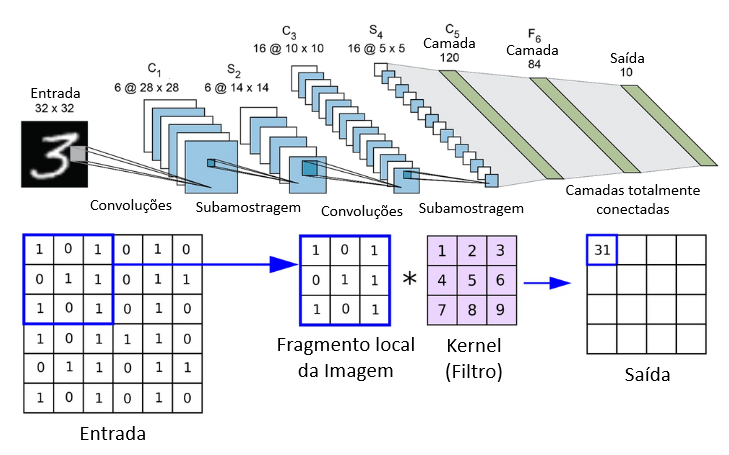
\includegraphics[width=1\linewidth]{conv_layers.png}
    \caption{Organização estrutural das camadas convolucionais em uma \acs{CNN}. O processo de convolução entre os filtros e as regiões locais da imagem permite a extração de padrões espaciais. À medida que a profundidade da rede aumenta, as representações tornam-se mais abstratas e informativas. Fonte: Adaptado de \cite{Jiang2024}.}
    \label{fig:conv_layers}
\end{figure}

A arquitetura de uma \acs{CNN} é composta por diferentes tipos de camadas, as quais são responsáveis por desempenhar uma função específica no processo de extração e interpretação das características visuais:

\begin{itemize}
    
    \item \textbf{Camada convolucional (\textit{convolutional layer}):} responsável pela aplicação de filtros (\textit{kernels}), representados por pequenas matrizes de pesos (geralmente de dimensões 3×3 ou 5×5), sobre a imagem de entrada. Durante o processo de convolução, esses filtros percorrem a imagem realizando operações locais de multiplicação e soma, das quais resultam mapas de características (\textit{feature maps}) que destacam padrões específicos presentes nos dados. Cada filtro tende a responder a determinadas características, como bordas, texturas ou formas elementares, e a utilização conjunta de múltiplos filtros permite a extração de representações cada vez mais informativas da imagem;
    
    \item \textbf{Camada de ativação:} introduz não linearidade ao modelo por meio de funções de ativação, permitindo que a rede aprenda relações complexas entre os dados. Sem essa etapa, a rede seria limitada a transformações lineares. Funções como \textit{\acs{ReLU}}, \textit{Sigmoid} e \textit{Tanh} são comumente utilizadas nesse contexto;
    
    \item \textbf{Camada de \textit{pooling} (subamostragem):} tem como objetivo reduzir as dimensões espaciais dos mapas de características, preservando as informações mais relevantes. Essa redução contribui para a diminuição do custo computacional e para a maior robustez do modelo a pequenas variações espaciais, como deslocamentos ou deformações;
    
    \item \textbf{Camadas totalmente conectadas (\textit{fully connected layers}):} nesta etapa, os mapas de características são convertidos em um vetor unidimensional por meio do processo de \textit{flattening}. Esse vetor é então utilizado como entrada para camadas densas, responsáveis por combinar as características extraídas e realizar a predição final, geralmente por meio de uma função de ativação como a \textit{softmax}, em problemas de classificação.

\end{itemize}

As \acsp{CNN} não seguem uma estrutura fixa, podendo ser adaptadas em termos de profundidade, número de filtros, tamanho dos \textit{kernels} e estratégias de conexão entre camadas. Essa flexibilidade arquitetural é uma de suas principais vantagens, permitindo sua aplicação em uma ampla variedade de problemas, desde tarefas simples de classificação até aplicações complexas em visão computacional.

Arquiteturas clássicas como \textit{AlexNet}, \textit{\acs{VGG}Net} e \textit{Inception} demonstram como diferentes estratégias de projeto podem impactar diretamente o desempenho e a escalabilidade dos modelos. Para um aprofundamento nos aspectos técnicos e nas variações arquiteturais das \acsp{CNN}, recomenda-se a literatura \textit{A review of convolutional neural networks in computer vision} \cite{zhao2024}. No contexto deste trabalho, arquiteturas convolucionais distintas foram exploradas para o problema de classificação proposto, com o objetivo de comparar seus desempenhos e identificar o modelo mais adequado para a condução dos experimentos finais.

\subsubsection*{Residual Network - ResNet}

A arquitetura \textit{ResNet} foi proposta com o objetivo de superar limitações observadas em \acsp{CNN} profundas, especialmente o problema do desaparecimento do gradiente (\textit{vanishing gradient}) e a degradação do desempenho à medida que a profundidade da rede aumenta. Em arquiteturas convencionais, o acréscimo de camadas pode dificultar o processo de otimização, resultando em piora da acurácia e instabilidade durante o treinamento, mesmo na ausência de \textit{overfitting}.

Neste contexto, a \textit{ResNet} introduz o conceito de aprendizado residual, o qual é implementado por meio dos chamados blocos residuais, que incorporam conexões de atalho (\textit{skip connections}) entre camadas. Em vez de aprender diretamente a transformação desejada, o modelo passa a aprender uma função residual — isto é, a diferença entre a entrada e a saída esperada. A saída do bloco é então obtida pela soma entre essa transformação e a entrada original.

Essa estratégia favorece a propagação do fluxo de informação e do gradiente ao longo da rede, reduzindo significativamente os efeitos do desaparecimento do gradiente e facilitando o processo de otimização geral. Além disso, as conexões residuais permitem que a rede preserve informações de camadas anteriores e, quando necessário, propague a entrada sem modificações relevantes, contribuindo para maior estabilidade e desempenho em redes profundas.

De forma geral, as arquiteturas da família \textit{ResNet} são organizadas em três componentes principais: o \textit{stem}, o \textit{backbone} e o \textit{head}. O \textit{stem} corresponde ao estágio inicial da rede, responsável por realizar as primeiras operações de extração de características a partir da imagem de entrada. Tipicamente, essa etapa inclui uma convolução inicial (frequentemente com filtros 7×7 e \textit{stride} 2), seguida por normalização em lote (\textit{Batch Normalization}), função de ativação \textit{\acs{ReLU}} e uma operação de \textit{pooling}. 

Os blocos residuais, por sua vez, constituem o núcleo da arquitetura. Existem dois tipos principais de blocos na família \textit{ResNet}: o bloco básico (\textit{basic block}), utilizado em redes mais rasas (como ResNet-18 e ResNet-34), e o bloco de gargalo (\textit{bottleneck}), empregado em redes mais profundas (como ResNet-50 e superiores). O \textit{basic block} é composto por duas camadas convolucionais $3\times3$, enquanto o bloco \textit{bottleneck} utiliza uma sequência de três convoluções ($1\times1$, $3\times3$, $1\times1$), com o objetivo de reduzir e posteriormente restaurar a dimensionalidade dos canais, tornando o modelo mais eficiente computacionalmente. Em ambos os casos, a saída do bloco é somada à entrada por meio de uma conexão residual.

Os blocos são organizados em estágios (conv2\_x, conv3\_x, conv4\_x e conv5\_x), nos quais a profundidade e o número de filtros aumentam progressivamente, permitindo a extração de representações cada vez mais abstratas. Por fim, a camada final (\textit{head}) é responsável pela etapa de classificação, na qual aplica-se uma operação de \textit{Global Average Pooling} a fim de reduzir cada mapa de características a um único valor, seguida por uma camada totalmente conectada para geração das predições finais. Nesta etapa, o funcionamento ocorre de modo análogo a uma \acs{DNN}, cumprindo o papel classificatório.

Embora variantes específicas — como \textit{ResNet}-18, \textit{ResNet}-34, \textit{ResNet}-50, \textit{ResNet}-101 e \textit{ResNet}-152 — diferenciem-se principalmente pela profundidade e pelo tipo de bloco utilizado, sua estrutura conceitual permanece consistente, permitindo a adaptação da arquitetura a diferentes cenários sem comprometer a filosofia de funcionamento. Como exemplo, a Figura \ref{fig:resnet50} ilustra a construção estrutural do modelo \textit{ResNet}-50, composto por 50 camadas treináveis organizadas nos estágios \textit{stem}, \textit{bottleneck} (conv2\_x,conv3\_x, conv4\_x, conv5\_x) e \textit{head}.

\begin{figure}[h]
    \centering
    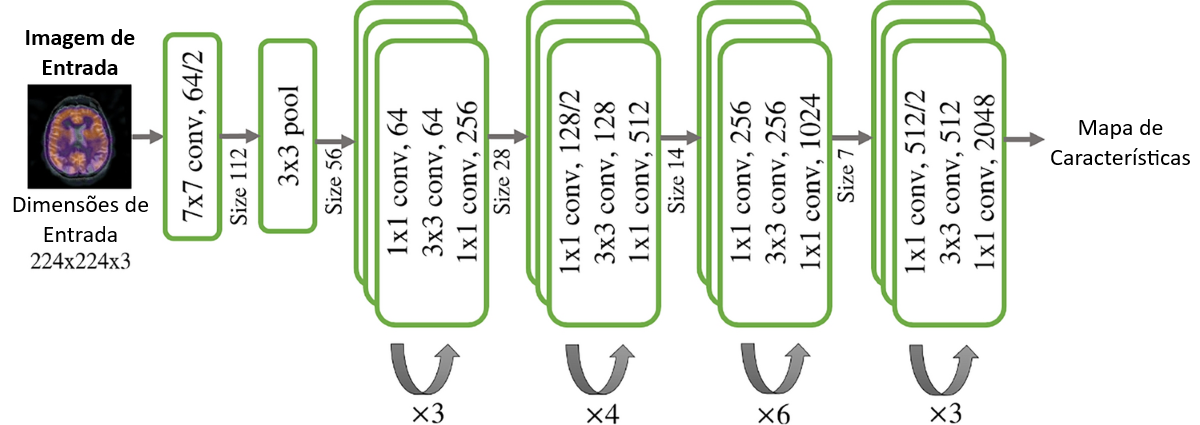
\includegraphics[width=1\linewidth]{resnet_50.png}
    \caption{Organização estrutural das camadas convolucionais no modelo \textit{ResNet50}. Fonte: Adaptado de \cite{Stack2025}.}
    \label{fig:resnet50}
\end{figure}

A arquitetura \textit{ResNet} teve um impacto significativo no avanço do aprendizado profundo, ao viabilizar o treinamento de redes com dezenas ou até centenas de camadas de forma estável. Sua proposta de aprendizado residual tornou-se um marco na área, influenciando o desenvolvimento de diversas extensões, como a \textit{ResNeXt}, que introduz o conceito de cardinalidade (múltiplos caminhos paralelos dentro dos blocos), a \textit{Wide ResNet}, que prioriza o aumento da largura da rede, e a \textit{ResNetV2}, que modifica a ordem das operações internas para melhorar a estabilidade do treinamento.  A estrutura descrita previamente, bem como a topologia padrão da arquiteura podem ser consultadas com maior detalhamento por meio do artigo \textit{Deep Residual Learning for Image Recognition} \cite{he2016}.

\subsubsection*{Densely Connected Convolutional Network - DenseNet}

A \textit{DenseNet} introduz um padrão de conectividade distinto no contexto das \acsp{CNN}, no qual cada camada recebe como entrada os mapas de características de todas as camadas anteriores dentro de um mesmo bloco \cite{Huang2017}, conforme ilustrado pela Figura \ref{fig:densenet_str}. Como consequência, cada camada tem acesso direto tanto a informações de baixo nível (como bordas e texturas) quanto a representações mais abstratas, aprendidas em camadas mais profundas. 

\begin{figure}[h]
	\centering
	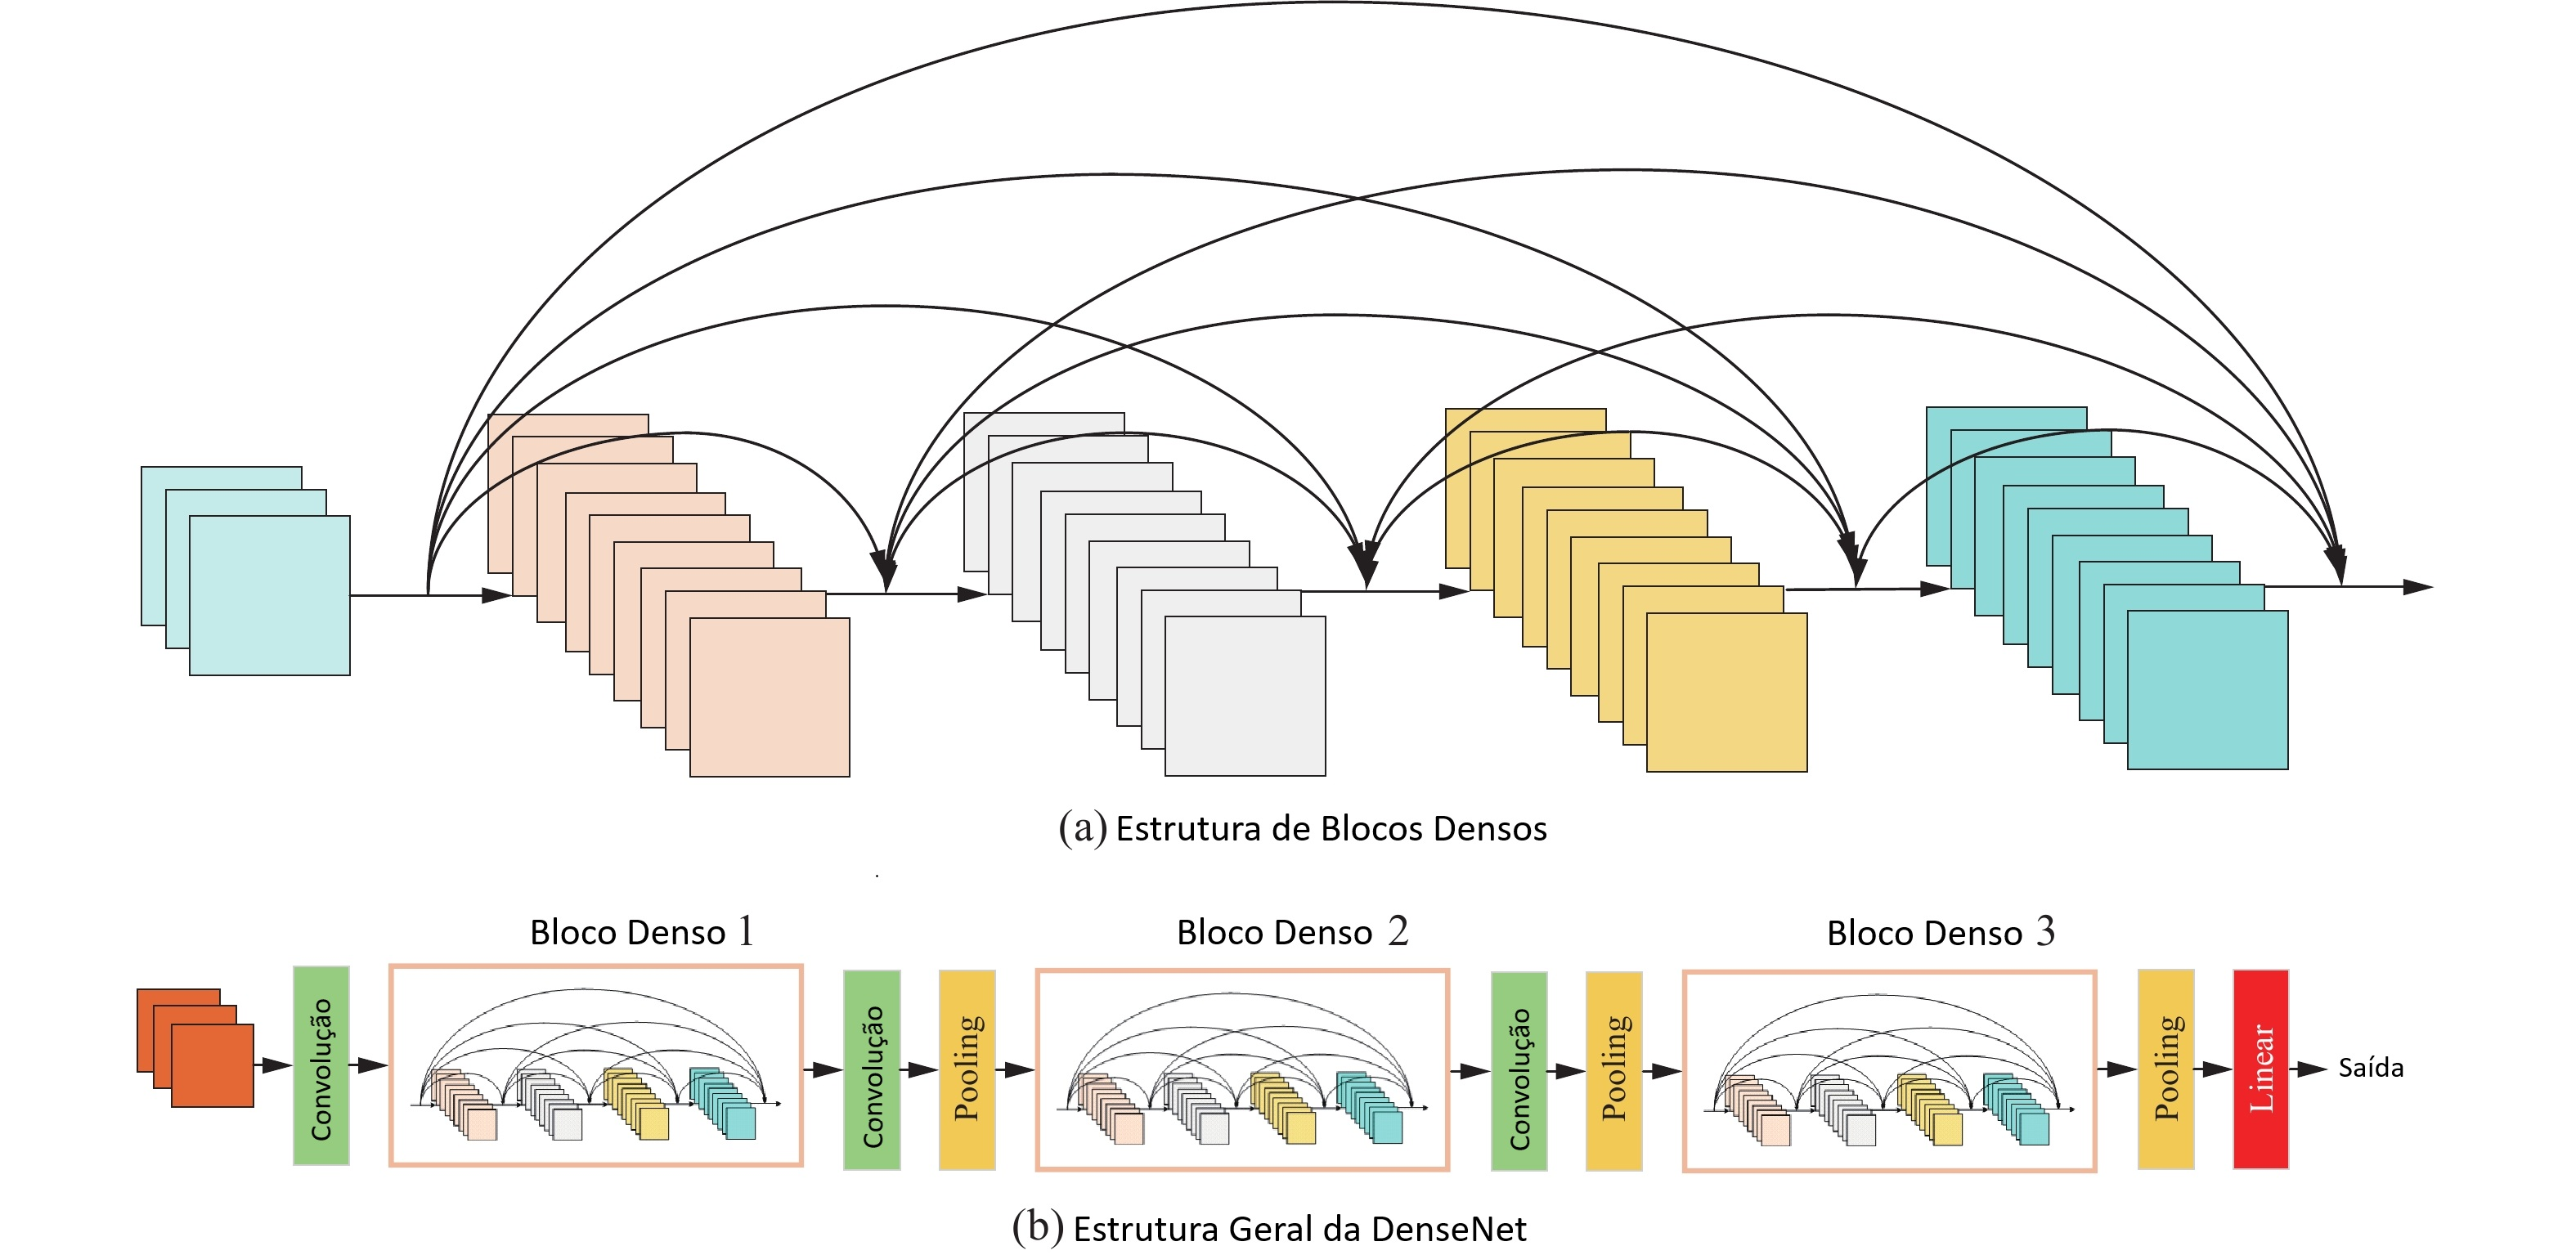
\includegraphics[width=0.9\linewidth]{figuras/figs_fundamentacao/DenseNet_Str}
	\caption{Estrutura da arquitetura \textit{DenseNet}, com destaque para o reaproveitamento completo de características entre as camadas. Fonte: Adaptado de \cite{jia2021cnn_palmprint}.}
	\label{fig:densenet_str}
\end{figure}

Diferentemente das \acsp{CNN} tradicionais, em que a informação flui de forma sequencial entre camadas adjacentes, a \textit{DenseNet} promove um fluxo de informação mais intenso e contínuo ao longo da rede, favorecendo um alto reaproveitamento de características e  contrastando diretamente com a abordagem adotada pela \textit{ResNet}, na qual as conexões residuais realizam somas entre entradas e saídas de blocos. Formalmente, considerando um bloco denso com $L$ camadas, a entrada da camada $l$ ($x_l$) é definida como a concatenação $H_l(\cdot\cdot\cdot)$ das saídas de todas as camadas anteriores, conforme descrito pela equação \ref{eq:denset_concat}. 

\begin{equation}
	\begin{aligned}
		\displaystyle x_l &= H_l([x_0, x_1, x_2, \dots, x_{l-1}]) \\[8pt]
		&\text{onde:} \\
		&x_l \rightarrow \text{entrada da camada } l \\
		&H_l \rightarrow \text{operação de concatenação das saídas anteriores}
	\end{aligned}
	\label{eq:denset_concat}
\end{equation}

Do ponto de vista estrutural, a DenseNet é organizada em blocos densos (\textit{dense blocks}), intercalados por camadas de transição (\textit{transition layers}). Dentro de cada bloco denso, múltiplas camadas convolucionais são empilhadas com conexões completas entre si. Já as camadas de transição são responsáveis por controlar o crescimento do número de canais e reduzir a dimensionalidade espacial dos mapas de características, sendo geralmente compostas por convoluções $1\times1$ seguidas de operações de \textit{pooling}.

Um conceito central na \textit{DenseNet} é a taxa de crescimento (\textit{growth rate}), que define quantos novos mapas de características cada camada adiciona ao conjunto global. Diferentemente de arquiteturas convencionais, em que o número de filtros pode crescer rapidamente, a \textit{DenseNet} mantém esse crescimento controlado, o que contribui para a eficiência do modelo em termos de número de parâmetros. 

A conectividade densa favorece a propagação do gradiente ao longo da rede, mitigando problemas como o desaparecimento do gradiente (\textit{vanishing gradient}), de maneira semelhante — porém estruturalmente distinta — à estratégia adotada pela ResNet. Além disso, o forte reaproveitamento de características reduz a necessidade de aprender representações redundantes, resultando em modelos mais compactos e eficientes.

No contexto deste trabalho, a \textit{DenseNet} foi incluída como uma alternativa arquitetural à ResNet, com o objetivo de investigar o impacto na priorização do reaproveitamento explícito de características, frente ao aprendizado residual oferecido pela \textit{ResNet}. Considerando o tamanho reduzido do conjunto de dados e a natureza sutil das variações faciais associadas à dor, a capacidade da DenseNet de preservar características de baixo nível ao longo de toda a rede pode favorecer a identificação de padrões finos, potencialmente contribuindo para uma melhor generalização.

\subsubsection*{Mobile Network - MobileNet}

A \textit{MobileNet} é uma arquitetura de rede neural convolucional leve, proposta por Howard et al. \cite{Howard2017}, com o objetivo de oferecer alta eficiência computacional em cenários com restrições de recursos, como dispositivos móveis e sistemas embarcados. Diferentemente de arquiteturas convencionais, que priorizam desempenho máximo mesmo à custa de alto custo computacional, a \textit{MobileNet} foi projetada com foco no equilíbrio entre acurácia e eficiência.

O principal diferencial da MobileNet está no uso de convoluções separáveis em profundidade (\textit{depthwise separable convolutions}), uma fatoração da convolução padrão que reduz significativamente o número de parâmetros e operações necessárias, conforme ilustrado pela Figura \ref{fig:mobilenetstr}. Em uma convolução tradicional, cada filtro atua simultaneamente sobre todas as dimensões espaciais e canais de entrada. Já na abordagem separável, essa operação é decomposta em duas etapas: uma convolução em profundidade (\textit{depthwise convolution}), que aplica um único filtro por canal de entrada, seguida por uma convolução ponto a ponto (\textit{pointwise convolution}, $1\times1$), responsável por combinar as informações entre os canais.

Enquanto uma convolução padrão possui custo proporcional a $D_k \times D_k \times M \times N$, sendo $D_k$ é o tamanho do kernel, $M$ o número de canais de entrada e $N$ o número de filtros, a convolução separável reduz esse custo para aproximadamente $D_k \times D_k \times M + M \times N$, resultando em uma economia significativa, especialmente em redes profundas.

\begin{figure}[h]
	\centering
	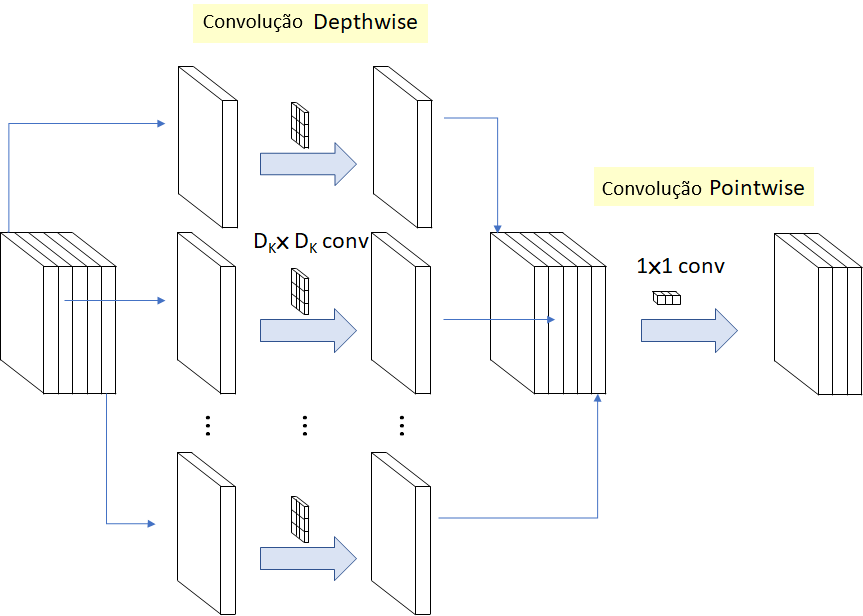
\includegraphics[width=0.7\linewidth]{figuras/figs_fundamentacao/MobileNet_str}
	\caption{Estrutura convolucional adotado pela \textit{MobileNet}, baseada em operações separáveis em profundidade. Fonte: Adaptado de \cite{tomar2021crowd}.}
	\label{fig:mobilenetstr}
\end{figure}

Adicionalmente, a \textit{MobileNet} introduz dois hiperparâmetros importantes que permitem ajustar o modelo conforme as restrições do problema: o multiplicador de largura (\textit{width multiplier}), que reduz proporcionalmente o número de canais em cada camada, e o multiplicador de resolução (\textit{resolution multiplier}), que diminui o tamanho espacial das imagens de entrada. Esses mecanismos oferecem flexibilidade para adaptar o modelo a diferentes cenários, controlando diretamente o trade-off entre custo computacional e desempenho.

Do ponto de vista estrutural, a MobileNet segue um padrão sequencial de camadas convolucionais separáveis, intercaladas com normalização em lote (\textit{Batch Normalization}) e funções de ativação não lineares, como a \textit{\acs{ReLU}}, conforme descrito pela tabela \ref{tab:mobilenet_str}. Diferentemente de arquiteturas como a \textit{ResNet} e a \textit{DenseNet}, a MobileNet não utiliza conexões residuais densas ou estratégias explícitas de reaproveitamento de características, priorizando uma arquitetura mais simples e eficiente.


\begin{table}[h]
	\centering
	\caption{Configuração estrutural do modelo MobileNet-V1, utilizado neste estudo.}
	\label{tab:mobilenet_str}
	\renewcommand{\arraystretch}{1.3}
	
	\begin{tabular}{l|l}
		\toprule
		\textbf{Camada} & \textbf{Estrutura} \\
		\midrule
		
		Conv1 & $3 \times 3$, 32, stride 2 \\        
		Conv2 (DW + PW) & Depthwise $3 \times 3$, stride 1 + Pointwise $1 \times 1$, 64 \\        
		Conv3 (DW + PW) & Depthwise $3 \times 3$, stride 2 + Pointwise $1 \times 1$, 128 \\        
		Conv4 (DW + PW) & Depthwise $3 \times 3$, stride 1 + Pointwise $1 \times 1$, 128 \\        
		Conv5 (DW + PW) & Depthwise $3 \times 3$, stride 2 + Pointwise $1 \times 1$, 256 \\
		Conv6 (DW + PW) & Depthwise $3 \times 3$, stride 1 + Pointwise $1 \times 1$, 256 \\
		Conv7 (DW + PW) & Depthwise $3 \times 3$, stride 2 + Pointwise $1 \times 1$, 512 \\
		
		Conv8--12 ($\times 5$) 
		& \makecell[l]{
			Depthwise $3 \times 3$, stride 1 \\
			Pointwise $1 \times 1$, 512
		}\\
		
		Conv13 (DW + PW) & Depthwise $3 \times 3$, stride 2 + Pointwise $1 \times 1$, 1024 \\
		Conv14 (DW + PW) & Depthwise $3 \times 3$, stride 1 + Pointwise $1 \times 1$, 1024 \\
		
		\midrule
		
		AvgPool & Global average pooling \\ 
		Dropout & 0.3 \\
		FC & Fully connected (3 classes, softmax) \\
		
		\bottomrule
	\end{tabular}
\end{table}

A \textit{MobileNet} apresenta um contraste importante com as demais arquiteturas analisadas neste trabalho. Enquanto a \textit{ResNet} utiliza conexões residuais para facilitar o fluxo de gradientes em redes profundas, e a \textit{DenseNet} promove o reaproveitamento intensivo de características por meio de conexões densas, a MobileNet adota uma abordagem focada na eficiência estrutural, reduzindo a complexidade das operações internas da rede. 

Neste estudo, a \textit{MobileNet} foi incorporada com o objetivo de avaliar a viabilidade da implementação de sistemas automatizados para detecção de dor em ambientes com restrições de recursos computacionais, buscando ampliar o acesso às ferramentas de monitoramento para o bem-estar animal. Por fim, a comparação entre os modelos convolucionais fornece uma visão abrangente sobre o impacto de diferentes paradigmas ao problema proposto.

\subsection{Transformers e Vision Transformers}

As \textit{Vision Transformers} representam um avanço significativo no campo da visão computacional, sendo uma adaptação dos \textit{Transformers}, uma arquitetura originalmente desenvolvida no campo do Processamento de Linguagem Natural (\acs{NLP}) que se baseia no mecanismo de autoatenção (\textit{self-attention}), responsável por permitir que o modelo aprenda as relações globais entre os elementos de entrada. Diferentemente de abordagens convencionais, que processam as dependências de forma sequencial e local, os \textit{Transformers} analisam todos os elementos simultaneamente, atribuindo diferentes níveis de importância a cada um. Essa característica possibilita a modelagem de dependências de longo alcance logo no inicio do processo, além de possibilitar um alto grau de paralelização durante o treinamento — aspectos fundamentais para o sucesso da arquitetura em tarefas como tradução automática, sumarização de textos e modelos de linguagem em larga escala.

As \acsp{VIT} seguem princípios muito semelhantes aos \textit{Transformers} empregados em \acs{NLP}. Para compreender o funcionamento do mecanismo de autoatenção, é interessante observar um exemplo do contexto linguístico. Considerando a frase: 'O gato subiu na mesa para comer o peixe', é correto afirmar que nem todas as palavras possuem o mesmo peso para a interpretação do significado geral. Ao analisar o verbo 'comer', por exemplo, o modelo precisa concentrar maior atenção nas palavras 'gato' e 'peixe', pois são elas que estabelecem a relação semântica mais relevante. O mecanismo de atenção, portanto, tem como objetivo atribuir pesos diferentes a cada elemento da sequência, de acordo com sua importância contextual, produzindo os denominados scores de atenção — valores que indicam a influência relativa de cada palavra em relação às demais. Dessa forma, o modelo consegue representar com precisão as relações globais existentes na sequência analisada.

A primeira etapa do processo consiste em converter o texto não estruturado em um formato compreensível para o modelo computacional. Para isso, são aplicadas duas técnicas fundamentais: \textit{tokenização} e \textit{embeddings}. A \textit{tokenização} corresponde à decomposição do texto em unidades menores, denominadas \textit{tokens}, que podem ser palavras, subpalavras, símbolos ou até caracteres individuais. Essa etapa transforma o fluxo contínuo de texto em uma sequência discreta de elementos analisáveis. Em seguida, cada token é convertido em uma representação vetorial contínua, denominada embedding, os quais mapeiam elementos semelhantes para pontos próximos em um espaço vetorial multidimensional, permitindo que o modelo capture relações semânticas e sintáticas entre tais elementos. No exemplo anterior, os \textit{tokens} 'gato' e 'peixe' teriam vetores próximos nesse espaço, pois compartilham semelhanças semânticas (ambos representam animais). Essas representações são aprendidas automaticamente durante o treinamento do modelo.

Adicionalmente, além do significado das palavras, o \textit{Transformer} também precisa compreender a posição de cada \textit{token} na sequência, já que, diferentemente das redes recorrentes, ele não processa as entradas em ordem temporal. Para isso, o modelo utiliza os \textit{embeddings} posicionais (\textit{positional embeddings}), vetores que codificam a posição de cada token na sequência. Assim, a entrada final para o modelo é obtida pela soma do \textit{embedding} do \textit{token} com seu respectivo \textit{embedding} posicional — uma combinação que permite ao \textit{Transformer} considerar simultaneamente o conteúdo e a posição dos elementos durante o processamento nas camadas de autoatenção.

Após a etapa de formatação e codificação posicional, os vetores de entrada são submetidos ao mecanismo de autoatenção, responsável por modelar as relações internas entre os diferentes tokens da sequência. O processo tem início com a projeção de cada token em três espaços vetoriais distintos, obtidos por meio de transformações lineares aprendíveis. Tais projeções dão origem a três matrizes fundamentais: Query (Q), Key (K) e Value (V); Cada uma exerce um papel específico na construção das relações de atenção entre os elementos:

\begin{itemize}
    \item \textbf{Vetor Q (Query)} 	$\rightarrow$ Representa a 'pergunta' que um token faz ao resto da sequência - 'o que eu preciso saber do contexto agora?';
    \item \textbf{Vetor K (Key)} 	$\rightarrow$ Funciona como uma 'chave' ou 'assinatura' associada a cada \textit{token}, descrevendo o tipo de informação que ele pode oferecer aos demais - “o que eu tenho para oferecer a quem me perguntar?”;
    \item \textbf{Vetor V (Value)} $\rightarrow$ Representa o conteúdo efetivo que será transmitido ou agregado quando um \textit{token} recebe atenção, correspondendo à informação contextual que compõe a nova representação final.
\end{itemize}

De forma mais intuitiva, o mecanismo de autoatenção consiste em medir quanto cada \textit{token} deve prestar atenção aos demais. Para isso, cada \textit{query} é comparada com todas as \textit{keys} da sequência, produzindo um conjunto de pesos que indicam o grau de relevância de cada \textit{token} em relação ao outro. Esses pesos são, então, utilizados para calcular uma combinação ponderada dos \textit{values}, gerando uma nova representação contextualizada para cada elemento de entrada. Formalmente, são usadas três matrizes de projeção $W_Q$, $W_K$, $W_V$ $\in R^{dXd_k}$. Tais matrizes são parâmetros treináveis, ou seja, o modelo ajusta essas projeções durante o treinamento para que a atenção aprenda relações úteis para a tarefa. Com isso, as matrizes Q, K e V são definidas por: $Q = XW_Q$; $K = XW_K$; $V = XW_V$ (Sendo X o vetor de embeddings). 

É importante destacar que as matrizes de projeção $W_Q$, $W_K$ e $W_V$ são necessárias por permitirem que o modelo aprenda subespaços de representação especializados para diferentes propósitos: buscar informações (Q), indexar elementos relevantes (K) e retornar o conteúdo contextualizado (V). Caso o próprio vetor de embedding fosse utilizado diretamente como query, key e value, o modelo ficaria restrito a um único espaço de representação, limitando sua capacidade de capturar relações complexas entre os tokens. As projeções lineares, ampliam a expressividade do modelo ao permitir que a atenção opere sobre perspectivas distintas do mesmo dado, como aspectos sintáticos, semânticos ou posicionais. De maneira mais didática, temos:

\begin{enumerate}
    \item \textbf{Separação de responsabilidades} 	$\rightarrow$ cada matriz de projeção tem uma função específica dentro do cálculo de atenção:
    \begin{itemize}
        \item $W_Q$ transforma cada $x_i$ num vetor que expressa o que esse \textit{token} está buscando compreender no contexto (sua “pergunta”);
        \item $W_K$ transforma cada $x_j$ num vetor que expressa o que o \textit{token} $j$ oferece como informação disponível (sua “assinatura”);
        \item $W_V$ projeta o vetor de entrada para o espaço do conteúdo efetivo que será transmitido e agregado (sua “resposta”).
    \end{itemize}
    \item \textbf{Mudança de base / subespaços:} as projeções criam subespaços vetoriais onde as relações de similaridade entre \textit{queries} e \textit{keys} tornam-se significativas para a tarefa. Por exemplo, um subespaço pode capturar padrões sintáticos (como dependências entre verbos e sujeitos), enquanto outro pode capturar relações semânticas (como associações entre conceitos relacionados). Essa separação facilita o aprendizado de múltiplas dimensões de significado dentro de uma mesma sequência.
\end{enumerate}

Com a definição das matrizes $Q$ e $K$, torna-se possível calcular as pontuações de atenção (\textit{attention scores}), que quantificam o grau de compatibilidade (atenção) entre cada par de \textit{tokens}. Matematicamente, o modelo compara cada vetor \textit{query} $Q_i$ com todos os vetores \textit{key} $K_j$ da sequência, por meio de um produto escalar, resultando em uma medida de similaridade entre $Q_i$ e $K_j$:

\begin{equation}
    Score(i,j) = Q_i \cdot K^T_j
\end{equation}

O resultado dessa operação para todos os elementos gera uma matriz de pontuações de atenção, em que cada valor $Score(i,j)$ representa o quanto o \textit{token} na posição $i$ deve considerar o \textit{token} na posição $j$ ao atualizar seu próprio estado. Entretanto, esses valores ainda não são probabilidades; tratam-se apenas de medidas numéricas de similaridade, que podem variar amplamente em escala.

Para que possam ser interpretadas como pesos de atenção normalizados, aplica-se a função \textit{Softmax} sobre cada linha dessa matriz, transformando as pontuações em valores positivos entre 0 e 1 cuja soma é igual a 1 (probabilidades). Isso garante que o modelo distribua sua atenção de maneira ponderada entre todos os \textit{tokens}. Adicionalmente, antes da aplicação da \textit{Softmax}, as pontuações são divididas por $\sqrt{d_k}$, onde $d_k$ corresponde à dimensionalidade dos vetores \textit{key}. Essa normalização tem a função de evitar que os produtos escalares cresçam excessivamente com o aumento da dimensionalidade, o que poderia tornar a \textit{Softmax}  sensível a pequenas variações numéricas e, consequentemente, gerar gradientes instáveis durante o treinamento. Matematicamente, temos:

\begin{equation}
    Attention \: Weights(i,j) = Softmax (\frac{Q_i . K^T_j}{\sqrt{d_k}})
\end{equation}

\begin{center}
    De forma simplificada, podemos representá-la também como:
\end{center}

\begin{equation}
    Attention \: Weights(i,j) = Softmax (\frac{Score(i,j)}{\sqrt{d_k}})
\end{equation}

Após essa etapa, o modelo sabe, para cada palavra da sequência, quais outros elementos são mais relevantes para sua interpretação no contexto global. Como exemplo, podemos considerar os seguintes pesos atribuídos aos \textit{tokens} da frase 'O gato comeu':

\begin{itemize}
\item Atenção em “O”: 0.05
\item Atenção em “gato”: 0.45
\item Atenção em “comeu” (ela mesma): 0.70
\end{itemize}

Esses valores indicam que a palavra “comeu” concentra a maior parte de sua atenção em si mesma (caracterizando o princípio da autoatenção), mas também atribui uma atenção significativa à palavra 'gato' (0.45), reconhecendo que ela é o sujeito da ação expressa pelo verbo. Por outro lado, a palavra 'O' recebe um peso pequeno (0.05), o que indica que sua contribuição semântica para a compreensão de “comeu” é menos relevante. 

Com os pesos calculados, o modelo realiza o passo final da autoatenção: a combinação ponderada dos vetores de valor (\textit{Value}). Cada vetor $V_j$ contém a informação contextual de um \textit{token} da sequência, e o peso de atenção $Attention : Weights(i,j)$, responsável por definir quanto dessa informação deve ser incorporada ao token $i$. O resultado é obtido pela soma ponderada de todos os \textit{Values}, dada pela seguinte expressão:

\begin{equation}
    Output(i) = \sum_j Attention \: Weights(i,j) \: \times \: V_j
\end{equation}

Assim, o vetor de saída $Output(i)$ representa uma versão contextualizada do \textit{token} $i$. Ele não reflete apenas a informação original da palavra, mas também agrega, de maneira ponderada, partes das informações de todas as outras palavras que receberam atenção. No exemplo anterior, a nova representação de 'comeu' passa a carregar não apenas a ideia de uma ação, mas também a noção de quem a executa (“gato”), enriquecendo a semântica do \textit{token}. Em contraste com arquiteturas sequenciais tradicionais, o \textit{Transformer} constrói simultaneamente todas as relações de atenção, resultando em representações altamente expressivas e interconectadas.

É importante destacar que, em modelos reais, o desempenho é mais expressivo quando o sistema é capaz de examinar diferentes tipos de relações entre os elementos de entrada simultaneamente. No entanto, isso não ocorre de forma plena quando o mecanismo de autoatenção é aplicado uma única vez. Nesse caso, o modelo tende a capturar uma única perspectiva das relações entre \textit{tokens}, ou seja, uma única métrica de similaridade em um único subespaço vetorial. 

Neste contexto introduz-se o conceito de \textit{multi-head attention}, cuja ideia central é calcular múltiplos mecanismos de atenção em paralelo, cada um operando em um subespaço distinto das representações de entrada, e posteriormente combinar os resultados obtidos. De forma intuitiva, seria como observar uma mesma cena por diferentes lentes: uma lente realça as cores, outra enfatiza contornos e outra destaca texturas. Ao combinar as observações de todas essas lentes, obtém-se uma representação mais rica do que qualquer lente isolada poderia oferecer.

Matematicamente, \textit{multi-head attention} divide a projeção total em $h$ cabeças. Em vez de projetar cada embedding $X$ de dimensão $d$ diretamente nos vetores Q, K e V de dimensões $d_k$, o mecanismo cria $h$ conjunto de matrizes $W^{(i)}_Q, W^{(i)}_K, W^{(i)}_V$ que projetam para subespaços de dimensão menor (normalmente $d_k = d/h$). Para cada cabeça $i$ calcula-se a atenção, sendo:

\begin{equation}
    head_i = Attention(Q^{(i)}, K^{(i)}, V^{(i)})
\end{equation}

\begin{center}
    Onde:
\end{center}

\begin{equation}
    Q^{(i)} = XW^{(i)}_Q; K = XW^{(i)}_K; V = XW^{(i)}_V
\end{equation}

Cada uma das saídas geradas por essas cabeças resulta em uma matriz de dimensão $n \times d_k$, que representa o número de \textit{tokens} ($n$) e a dimensão de cada subespaço ($d_k$). Em seguida, todas as saídas são concatenadas para formar uma única matriz de dimensão $n \times (h \cdot d_k)$ e, por fim, projetadas novamente em um espaço de dimensão $d$ por meio de uma matriz de projeção final $W_O \in R^{(h d_k) \times d}$, obtendo-se assim a saída consolidada da camada de atenção:

\begin{equation}
    MultiHead(X) = Concat(head_1,\ldots,head_h)W_o.
\end{equation}

A arquitetura dos \textit{Transformers} é composta por blocos modulares empilhados, que combinam mecanismos de atenção com camadas \textit{feedforward}, normalização e conexões residuais. Essa estrutura caracteriza o \textit{encoder} do modelo e permite o aprendizado eficiente de dependências complexas entre os elementos da entrada. Cada camada do \textit{encoder} realiza duas operações principais, executadas em sequência:

\begin{enumerate}
    \item Uma subcamada de atenção (tipicamente a \textit{multi-head self-attention}) que permite que cada posição da sequência acesse informações provenientes de todas as demais, capturando relações globais entre os elementos;
    \item Uma subcamada \textit{feedforward} aplicada após a atenção, que executa transformações ponto a ponto de forma independente para cada posição. Entre essas subcamadas, são inseridas conexões residuais (\textit{skip connections}) e mecanismos de normalização (geralmente\textit{ Layer Normalization} ou \textit{LayerNorm}).
\end{enumerate}

A subcamada \textit{feedforward} corresponde, na prática, a uma pequena rede neural densamente conectada, aplicada individualmente a cada \textit{token}. Em geral, ela é composta por duas projeções lineares separadas por uma função de ativação não linear (como \acs{ReLU} ou \acs{GELU}). Essa etapa amplia a capacidade de modelagem local das representações: enquanto o mecanismo de atenção redistribui informações entre diferentes posições, a camada densa permite que cada posição refine e recombine suas próprias características de maneira não linear, enriquecendo a representação antes que ela seja propagada para a próxima camada.

As conexões residuais e a normalização são cruciais para viabilizar o empilhamento profundo de blocos. A conexão residual adiciona a entrada de uma subcamada à sua saída (De maneira similar à arquitetura \textit{ResNet}), o que facilita o fluxo de gradiente durante o treinamento e permite que camadas extras não degradem o desempenho. Em seguida, aplica-se a normalização, a fim de estabilizar a distribuição das ativações, melhorar a convergência e favorecer a precisão do treinamento.

Na aplicação original, a arquitetura dos \textit{Transformers} é composta por dois componentes principais: o \textit{encoder} e o \textit{decoder}. O \textit{encoder} é responsável por processar a sequência de entrada, extraindo e representando suas características em um espaço vetorial de maior expressividade. Já o \textit{decoder} utiliza essas representações para gerar uma sequência de saída, etapa essencial em tarefas como tradução automática ou geração de texto. Recomenda-se a leitura do artigo \textit{Attention Is All You Need} \cite{vaswani2017}, que apresenta em detalhes a topologia padrão dos \textit{transformers} e o funcionamento do mecanismo de atenção, sendo este, a literatura responsável por introduzir o conceito.

Nas \acsp{VIT}, o processo segue a mesma filosofia dos \textit{Transformers} originais, mas é adaptado ao domínio visual. Nesse caso, a entrada não é uma sequência de palavras, mas sim uma sequência de \textit{patches}, que representam pequenas regiões extraídas da imagem, como exemplo: em uma imagem de dimensões $224 \times 224$ \textit{pixels}, é comum dividir o conteúdo em blocos de $16 \times 16$ \textit{pixels}, o que resulta em 196 \textit{patches}. Cada um desses blocos é achatado (vetorizado) e projetado linearmente em um vetor de \textit{embedding} de dimensão fixa.

São adicionados dois elementos fundamentais à sequência de embeddings dos patches: um token de classe (\textit{class token}), que agrega a informação global da imagem e serve como representação final para tarefas de classificação, e os \textit{embeddings} posicionais, responsáveis por fornecer à rede uma noção explícita de localização espacial (Análogo ao \textit{positional encoding} das \acsp{NLP}). A sequência resultante é então processada pelo \textit{encoder} do \textit{Transformer}, cujos blocos de atenção permitem que cada patch troque informações com todos os outros, capturando dependências espaciais de longo alcance. As redes \textit{feedforward} subsequentes, por sua vez, refinam as representações locais de cada \textit{patch}, complementando a informação contextual aprendida pela atenção. Recomenda-se a leitura do artigo \textit{An Image is Worth 16x16 Words: Transformers for Image Recognition at Scale} \cite{dosovitskiy2020vit} para obter maiores detalhes técnicos acerca da construção e implementação das \acsp{VIT}, sendo esta a literatura original responsável por apresentar a técnica.

\begin{figure}[h]
    \centering
    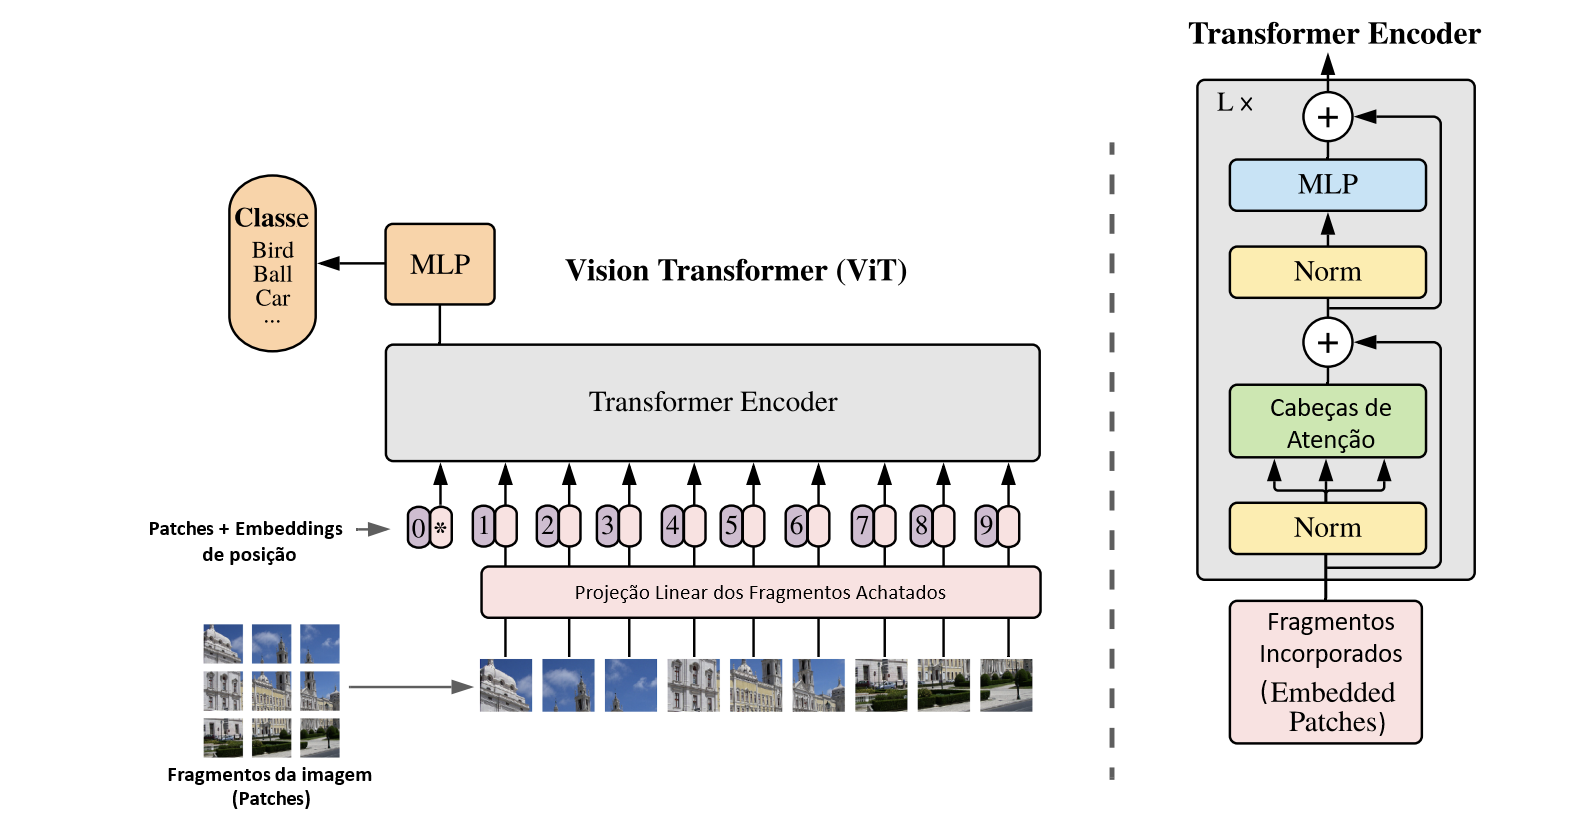
\includegraphics[width=1\linewidth]{vision_transformers.png}
    \caption{Topologia da arquiteura \textit{Vision Transformer}. Fonte: Adaptado de \cite{Huang2023}.}
    \label{fig:vit_topologia}
\end{figure}

A Figura \ref{fig:vit_topologia} ilustra de forma esquemática a topologia padrão da arquitetura \textit{Vision Transformer}, conforme descrita na literatura. A seguir, apresenta-se uma descrição intuitiva de sua estrutura, bem como a configuração de seus principais componentes e hiperparâmetros:

\begin{enumerate}

    \item \textbf{\textit{Input}:}
    \begin{itemize}
        \item A imagem de entrada possui dimensões $224\times224\times3$, correspondendo a imagens coloridas RGB (com 3 camadas) de resolução padrão;
        \item Cada imagem é dividida em \textit{patches} não sobrepostos de tamanho $16\times16$, resultando em $196$ \textit{patches} distintos;
        \item Cada \textit{patch} é achatado (\textit{flattened}) e projetado linearmente e formar o espaço de embeddings
    \end{itemize}
    
    \item \textbf{\textit{Patch Embedding} e \textit{Positional Encoding}:}
    \begin{itemize}
        \item Cada \textit{patch} é transformado por uma camada linear (projeção aprendível) que mapeia o vetor achatado de dimensão $16\times16\times3 = 768$ para um espaço de embedding de mesma dimensão ($d=768$);
        \item Um vetor adicional denominado \textit{class token} [CLS] é concatenado ao início da sequência de \textit{patches}, a fim de agregar a informação global da imagem;
        \item São adicionados embeddings posicionais aprendíveis (\textit{learnable positional embeddings}) aos vetores de entrada, preservando a informação espacial.
    \end{itemize}

    \item \textbf{\textit{Transformer Encoder}:}
    \begin{itemize}
        \item O modelo padrão \acs{VIT} é composto por 12 blocos de \textit{Transformer Encoder}, cada um contendo duas subcamadas principais: 
        \textit{(i)} \textit{Multi-Head Self-Attention} (\acs{MHSA}) e 
        \textit{(ii)} \textit{Feed-Forward Network} (\acs{FFN}), ambas com conexões residuais e normalização de camada (\textit{LayerNorm});
        \item Cada bloco utiliza 12 cabeças de atenção, cada uma com dimensão de 64, totalizando $12\times64 = 768$ dimensões, correspondendo à dimensão do embedding;
        \item A subcamada \textit{Feed-Forward} interna (\acs{MLP}) é composta por duas camadas densas com ativação não linear \acs{GELU}, sendo a primeira de dimensão $4d = 3072$ e a segunda de dimensão $d = 768$;
        \item É aplicado \textit{dropout} de 0.1 nas conexões e ativações para reduzir o risco de \textit{overfitting};
        \item O modelo é otimizado com o algoritmo \textit{AdamW}, utilizando \textit{learning rate} inicial de 0.001 e \textit{warmup} nas primeiras iterações, conforme recomendado para estabilizar o treinamento de arquiteturas baseadas em atenção.
    \end{itemize}

    \item \textbf{\textit{Class Token} e \textit{\acs{MLP} Head}:}
    \begin{itemize}
        \item Após o processamento pelos blocos do \textit{encoder}, o vetor correspondente ao \textit{class token} [CLS] é extraído como representação global da imagem;
        \item Esse vetor é passado por uma camada \textit{LayerNorm} e posteriormente por uma cabeça de classificação (\textit{\acs{MLP} Head}), composta por uma ou mais camadas densas, cuja saída é dimensionada conforme o número de classes da tarefa;
        \item A ativação final geralmente é do tipo \textit{Softmax}, produzindo uma distribuição de probabilidades sobre as classes.
    \end{itemize}

\end{enumerate}

É importante também reconhecer limitações e considerações deste tipo de arquitetura. O custo computacional do mecanismo de autoatenção cresce quadraticamente em relação ao número de \textit{patches}, o que pode tornar o treinamento inviável para imagens de alta resolução. Além disso, modelos baseados em \textit{Transformers} costumam demandar grandes volumes de dados para alcançar bom desempenho quando treinados do zero, exigindo estratégias adicionais de regularização, ajustes de taxa de aprendizado e inicialização criteriosa dos parâmetros para garantir estabilidade e convergência adequadas.

\section{Transfer Learning}

As redes neurais profundas são projetadas para aprender hierarquias de representações, em que as camadas iniciais capturam padrões visuais de baixa complexidade, como bordas e texturas, as camadas intermediárias identificam composições locais e as camadas finais abstraem conceitos de alto nível. Como muitos desses padrões de baixo e médio nível são compartilhados entre diferentes domínios visuais, o seu reaproveitamento reduz a carga de aprendizado sobre o conjunto de dados alvo. Nesse contexto, insere-se o conceito de aprendizado por transferência (\textit{Transfer Learning}).

O \textit{Transfer Learning} refere-se ao conjunto de técnicas que visam aproveitar o conhecimento adquirido por um modelo durante o treinamento em uma tarefa-fonte para melhorar o desempenho em uma tarefa-alvo, geralmente mais específica ou com menor volume de dados. A ideia central consiste em reutilizar representações previamente aprendidas (como pesos, filtros e \textit{embeddings}) provenientes de uma base de dados rica e diversa, a fim de acelerar o treinamento, reduzir a necessidade de rotulagem extensiva e aprimorar a capacidade de generalização do modelo em contextos de dados limitados.

No campo da visão computacional, o aprendizado por transferência tem se mostrado vantajoso em cenários nos quais o conjunto de dados é considerado pequeno (até 10.000 imagens) ou moderado (entre 10.000 e 100.000 imagens). Nesses casos, o esforço computacional é concentrado nas especifidades da atividade proposta, o que agiliza a convergência e evita redundâncias. No contexto deste estudo, por exemplo, a inicialização do modelo com pesos pré-treinados na base \textit{ImageNet} — um conjunto massivo composto por aproximadamente 1,2 milhão de imagens distribuídas em 1.000 categorias — permite que o processo de treinamento concentre-se na extração de características específicas e relevantes para a detecção de dor em camundongos, evitando o custo de aprendizado redundante das estruturas visuais fundamentais.

Existem duas estratégias amplamente utilizadas para a implementação do \textit{Transfer Learning}, baseadas no seguinte questionamento: “quanto do modelo original deve ser reaproveitado e quanto deve ser re-treinado?”. São elas:

\begin{enumerate}

    \item \textbf{\textit{Feature Extraction} (ou \textit{Linear Probing})}: consiste em uma abordagem mais simples e conservadora do aprendizado por transferência, na qual o modelo pré-treinado é utilizado apenas como extrator de características, sem que seus pesos internos sejam modificados. Na prática, o modelo é 'congelado', ou seja, todas as suas camadas permanecem fixas, e apenas uma nova camada final (classificadora) é adicionada e treinada. Essa camada costuma ser uma rede densa totalmente conectada com número de neurônios igual à quantidade de classes da nova tarefa.

    Como exemplo, pode-se considerar um modelo baseado na \textit{ResNet-50} pré-treinada na base \textit{ImageNet}. Nesse caso, a última camada que originalmente é responsável por classificar 1.000 categorias, é removida e substituída por uma nova camada com três saídas, adequando o modelo a uma tarefa de classificação para três classes distintas. Durante o treinamento, apenas os pesos da nova camada são atualizados, de modo que o modelo aprende apenas a interpretar as \textit{features} (características) já extraídas pelas camadas anteriores, sem modificar o processo de extração em si.

    Essa estratégia apresenta como principais vantagens o baixo custo computacional e o treinamento mais rápido, devido à menor quantidade de parâmetros ajustáveis. Entretanto, as \textit{features} aprendidas na tarefa original podem não ser totalmente adequadas à nova aplicação, o que pode limitar a capacidade de adaptação do modelo ao novo domínio.

    \item \textbf{\textit{Fine-tuning}}: trata-se de uma abordagem mais flexível, na qual parte (ou toda) a rede pré-treinada é re-treinada, permitindo o ajuste de seus pesos com base no novo conjunto de dados. A ideia é inicializar o treinamento a partir de um modelo já pré-treinado, mas, diferentemente da estratégia anterior, um subconjunto das camadas é descongelado (geralmente as últimas) para que seus pesos sejam refinados durante o processo de otimização. Dessa forma, o modelo preserva os conhecimentos gerais aprendidos (como bordas, texturas e formas), mas também passa a incorporar nuances específicas do novo domínio.

    O \textit{fine-tuning} oferece uma adaptação mais profunda ao novo domínio, permitindo ao modelo refinar suas representações internas para capturar padrões particulares da tarefa. Entretanto, o treinamento se torna computacionalmente mais caro e há maior risco de \textit{overfitting}, especialmente quando o conjunto de dados disponível é pequeno.
   
\end{enumerate}

\begin{figure}[h]
    \centering
    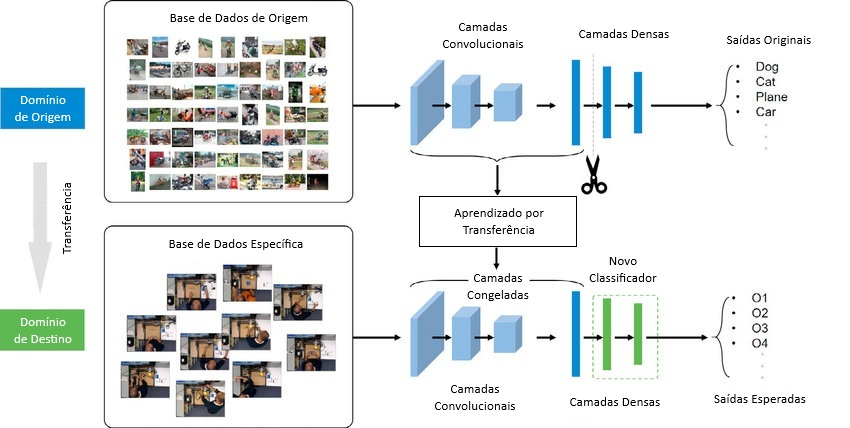
\includegraphics[width=1\linewidth]{transfer_learning_model.png}
    \caption{Exemplo intuitivo do \textit{transfer learning}, combinando o \textit{Linear Probing} com o \textit{Fine-tuning}. Fonte: Adaptado de \cite{Prabha2021}.}
    \label{fig:transfer_learning}
\end{figure}

Na prática, é comum combinar as duas estratégias descritas de forma sequencial. A Figura \ref{fig:transfer_learning} demonstra a aplicação inicial do \textit{Linear Probing} para treinar apenas a nova camada de classificação, garantindo estabilidade ao modelo. Em seguida, é feito o \textit{Fine-tuning} progressivo, no qual algumas camadas superiores são gradualmente descongeladas, e o treinamento continua com uma taxa de aprendizado reduzida. Essa abordagem é conhecida como \textit{progressive fine-tuning} ou \textit{two-stage transfer learning} e tende a produzir os melhores resultados, pois evita a instabilidade inicial de re-treinar toda a rede de uma só vez e promove uma adaptação mais controlada e eficiente ao novo domínio. Para maiores detalhes técnicos sobre a técnica de aprendizagem por transferência e as diferentes estratégias de aplicação, recomenda-se a leitura dos artigos \textit{A survey on transfer learning} \cite{pan2010},  e \textit{Fine-Tuning can Distort Pretrained Features and Underperform Out-of-Distribution} \cite{kumar2022finetuning}.

\section{TensorFlow}

Levando em consideração os objetivos deste projeto, uma ferramenta essencial para o desenvolvimento das tarefas relacionadas ao campo de inteligência artificial foi o \textit{TensorFlow}, um \textit{framework} de código aberto voltado à computação numérica e ao aprendizado de máquina, desenvolvido pelo \textit{Google}. Essa ferramenta foi projetada para expressar e executar fluxos de dados numéricos de forma eficiente e escalável. O \textit{TensorFlow} abrange tanto componentes de baixo nível, como operações tensorais, cálculo automático de gradientes e execução simbólica; quanto interfaces de alto nível, como a \acs{API} \textit{tf.keras}, que simplifica a construção e o treinamento de redes neurais.

A ideia central dessa ferramenta está na representação dos dados por meio de tensores (\textit{arrays} multidimensionais) e na descrição das operações matemáticas como nós interconectados em um grafo computacional. Esse paradigma permite que os modelos sejam definidos de maneira declarativa (especificando 'o que calcular' em vez de 'como calcular') e executados de forma paralela e otimizada em dispositivos distintos como \acs{CPU} e \acs{GPU}, sem a necessidade de alterar sua estrutura lógica. De modo geral, os tensores estão presentes em praticamente todas as etapas do processo de aprendizado, desempenhando diferentes funções dentro do fluxo de dados do modelo:

\begin{itemize}
    \item \textbf{Entradas:} os dados de entrada (imagens, textos, séries temporais) são convertidos em tensores para que possam ser processados pelas camadas subsequentes da rede;

    \item \textbf{Pesos (\textit{weights}):} cada camada da rede possui tensores treináveis, que representam os parâmetros internos (pesos e vieses) ajustados durante o processo de aprendizado;

    \item \textbf{Ativações:} os resultados intermediários (saídas produzidas por cada camada) também são tensores, os quais passam por funções de ativação (como \textit{\acs{ReLU}} ou \textit{Sigmoid}) responsáveis por introduzir não-linearidades no modelo;

    \item \textbf{Gradientes:} durante o treinamento, o \textit{TensorFlow} calcula automaticamente os tensores de gradiente, ou seja, as derivadas parciais da função de perda em relação a cada parâmetro da rede, permitindo a retropropagação do erro.
\end{itemize}

Tensores podem ser definidos como estruturas matemáticas que generalizam os conceitos de escalar, vetor e matriz para dimensões superiores. Intuitivamente, cada tensor é um \textit{array} multidimensional que armazena valores numéricos (sejam eles, inteiros, reais ou complexos) e que pode ser processado por operações matemáticas otimizadas em hardware. É importante destacar que os tensores não alteram as propriedades fundamentais das representações originais, apenas as estendem para um formato mais geral e flexível. Cada tensor é descrito essencialmente por três características principais:

\begin{enumerate}

    \item \textbf{\textit{Rank} (ordem):} indica o número de dimensões ou eixos que compõem o tensor. Essa propriedade permite compreender os tensores como extensões naturais das estruturas matemáticas básicas:


    \begin{itemize}

        \item Escalares (\textit{rank-0 tensors}) $\rightarrow$ representam um único valor numérico;

        \item Vetores (\textit{rank-1 tensors}) $\rightarrow$ representam uma sequência unidimensional de valores;
    
        \item Matrizes (\textit{rank-2 tensors}) $\rightarrow$ são usadas, para representar lotes de dados tabulares bidimensionais ou transformações lineares entre camadas;

        \item Matrizes (\textit{rank-2 tensors}) $\rightarrow$ representam dados bidimensionais, frequentemente utilizados para armazenar dados tabulares ou realizar transformações lineares entre camadas;

        \item Tensores de ordem superior (\textit{rank} $\geq$ 3) $\rightarrow$ são utilizados em domínios como visão computacional, representando imagens (3D — altura, largura e canais de cor), vídeos (4D — adicionando a dimensão temporal) e dados volumétricos (5D ou mais).

    \end{itemize}

    \item \textbf{\textit{Shape} (forma):} define o tamanho e a organização dos tensores em relação às suas dimensões. Por exemplo, um tensor com $shape = (4, 3)$ representa uma matriz composta por quatro linhas e três colunas.

    \item \textbf{Tipo de dado (\textit{dtype}):} especifica o tipo dos elementos armazenados no tensor, como \textit{float32}, \textit{int64} ou outros tipos compatíveis com o hardware de execução.

\end{enumerate}

Essas propriedades permitem que o \textit{TensorFlow} (ou qualquer outra biblioteca voltada ao \textit{deep learning}) interprete automaticamente como realizar operações entre tensores de tamanhos e tipos distintos, otimizando a alocação de memória e o paralelismo. Em sua estrutura interna, as operações sobre tensores são representadas como nós de um grafo computacional, enquanto os próprios tensores funcionam como arestas que transportam dados entre esses nós. 

Como exemplo: supondo a operação de multiplicação matricial $Z = XW + b$, os tensores $X$, $W$ e $b$ representam, respectivamente, as entradas, os pesos e o viés da transformação, resultando em um novo tensor $Z$. Durante o treinamento, cada operação armazena informações sobre o caminho computacional percorrido, permitindo ao \textit{TensorFlow} calcular automaticamente os gradientes necessários para a retropropagação do erro. Para uma descrição mais aprofundada das propriedades e operações sobre tensores, recomenda-se a consulta ao artigo de referência \textit{Tensor Decompositions and Applications} \cite{kolda2009tensor}.

O \textit{TensorFlow} disponibiliza um vasto conjunto de operações destinadas à manipulação de tensores, à execução de cálculos numéricos e ao gerenciamento de fluxos computacionais, abstraindo parte significativa da complexidade envolvida na implementação de modelos de aprendizado de máquina.Tais ferramentas tornam o \textit{framework} adequado tanto para pesquisas experimentais quanto para aplicações em larga escala, desde a etapa de prototipagem até a implantação em produção. Dentre as principais funcionalidades, destacam-se:

\begin{itemize}

    \item \textbf{Transformações estruturais:} englobam funções que permitem alterar a forma ou a organização dos tensores sem modificar seu conteúdo, possibilitando adaptações eficientes entre diferentes etapas de processamento. Entre as mais utilizadas estão: \texttt{reshape()}, \texttt{transpose()}, \texttt{concat()} e \texttt{stack()};

    \item \textbf{Operações matemáticas:} reúnem funções destinadas à realização de cálculos numéricos elementares ou compostos entre tensores, como multiplicação matricial (\texttt{matmul()}), soma (\texttt{add()}), subtração (\texttt{subtract()}), cálculo de médias (\texttt{reduce\_mean()}), entre outras;

    \item \textbf{Indexação e \textit{slicing}:} permitem acessar ou manipular regiões específicas de um tensor, de maneira análoga ao que ocorre com \textit{arrays} na biblioteca \textit{NumPy}, favorecendo o controle detalhado sobre subconjuntos de dados durante o processamento;

    \item \textbf{Broadcasting:} mecanismo que viabiliza a execução de operações entre tensores de dimensões distintas, ajustando automaticamente as dimensões de menor ordem para compatibilidade. Esse recurso é amplamente empregado em operações vetoriais e matriciais;

    \item \textbf{API para modelagem:} integra a \acs{API} \textit{Keras}, que fornece uma interface de alto nível voltada à definição, compilação e treinamento de modelos de aprendizado profundo. O \textit{Keras} padroniza a criação de camadas, funções de perda, métricas e ciclos de treinamento, além de oferecer métodos prontos para uso, como \texttt{Model.fit()} (treinamento), \texttt{Model.evaluate()} (avaliação de desempenho) e \texttt{Model.predict()} (inferência sobre novos dados), com suporte a \textit{callbacks} e registros de execução;

    \item \textbf{Otimizadores, funções de perda e métricas:} integração de algoritmos de otimização, incluindo \textit{\acs{SGD}}, \textit{Adam}, \textit{AdamW} e \textit{RMSProp}, além de funções de perda clássicas, como \textit{cross-entropy}, \textit{mean squared error (\acs{MSE})} e \textit{Huber loss}. Adicionalmente, o framework oferece métricas de desempenho como \textit{accuracy}, \textit{precision}, \textit{recall} e \textit{\acs{AUC}}, fundamentais para o acompanhamento da evolução do treinamento.
    
    \item \textbf{Distribuição e escalabilidade:} disposição de ferramentas para o treinamento distribuído, que realizam sincronização de gradientes, divisão de lotes de dados e gerenciamento de recursos computacionais, permitindo que modelos sejam treinados de forma eficiente em múltiplas \acsp{GPU}, \acsp{TPU} ou máquinas distintas, sem necessidade de alterações significativas na \acs{API};

    \item \textbf{Implantação e produção:} oferece suporte nativo à exportação e execução de modelos em diferentes ambientes, por meio de ferramentas como \textit{SavedModel} (formato padrão de exportação, preservando pesos e assinaturas de entrada/saída), \textit{TensorFlow Lite} (otimização para dispositivos móveis e embarcados) e \textit{TensorFlow.js} (execução direta em navegadores web);

    \item \textbf{Reutilização de conhecimento e monitoramento:} o \textit{Keras} também fornece acesso simplificado a modelos e pesos pré-treinados, viabilizando o uso de técnicas de \textit{transfer learning}. Adicionalmente, o \textit{TensorBoard} pode ser integrado ao processo de treinamento por meio de \textit{callbacks} e registros automáticos de \textit{logs}, permitindo a visualização de métricas, histogramas, imagens e embeddings em tempo real.

\end{itemize}

Em suma, o  \textit{TensorFlow} configura-se como uma plataforma completa voltada à pesquisa e à aplicação prática em aprendizado de máquina. Seu ecossistema abrange desde operações fundamentais sobre tensores até recursos avançados de treinamento distribuído, monitoramento e implantação de modelos em produção. Para maiores detalhes técnicos acerca das funcionalidades do \textit{Tensorflow}, recomenda-se a consulta do artigo \textit{TensorFlow: Large-Scale Machine Learning on Heterogeneous Distributed Systems} \cite{abadi2016tensorflow}.


\begin{comment}
	
	\section{Métricas para avaliação de resultados}
	
	Os resultados obtidos durante a experimentação científica exigem um processo de avaliação sólido e sistemático, de modo a verificar o comportamento e a eficácia dos modelos desenvolvidos. A aplicação de métricas e ferramentas de avaliação permitem mensurar o desempenho e a capacidade de generalização do modelo, além de reduzir o risco de interpretações imprecisas e orientar a tomada de decisões fundamentadas. 
	
	Dentre as ferramentas mais utilizadas para análise de desempenho em tarefas de classificação, destaca-se a Matriz de Confusão, uma estrutura tabular que compara as previsões realizadas pelo modelo com os valores reais das classes. Essa matriz fornece uma visão detalhada dos acertos e erros cometidos, sendo amplamente empregada para avaliar a confiabilidade e a robustez de classificadores supervisionados. A matriz é composta por quatro elementos fundamentais, que representam as possíveis combinações entre os rótulos reais e as previsões realizadas pelo modelo:
	
	\begin{itemize}
		\item \textbf{Verdadeiros positivos (\textit{True positive} - TP)}: casos rotulados como verdadeiros, que foram corretamente previstos;
		\item \textbf{Verdadeiros negativos (\textit{True Negatives} - TN)}: casos rotulados como negativos que corretamente previstos;
		\item \textbf{Falsos positivos (\textit{False Positive} - FP)}: casos negativos classificados como positivos (indica um alarme falso);
		\item \textbf{Falsos negativos (\textit{False Netgative} - FN)}: casos positivos classificados como negativos (indica uma falha de detecção do modelo).
	\end{itemize}
	
	A construção da matriz de confusão segue o princípio de que as \textbf{linhas} representam as classes reais e as \textbf{colunas} representam as classes previstas. Dessa forma, cada célula $(i, j)$ contém a quantidade de amostras cuja classe real é $i$ e que foram classificadas como pertencentes à classe $j$. Essa disposição permite identificar padrões de erro e compreender quais classes apresentam maior confusão entre si. Como exemplo, temos:
	
	\begin{table}[H]
		\centering
		\caption{Matriz de confusão ilustrativa para classificação binária}
		\label{tab:matriz_confusao}
		\renewcommand{\arraystretch}{1.8} % Aumenta o espaçamento entre linhas
		\setlength{\tabcolsep}{12pt} % Aumenta o espaçamento horizontal entre colunas
		\begin{tabular}{|c|c|c|c|}
			\hline
			\multicolumn{2}{|c|}{} & \multicolumn{2}{c|}{\textbf{Valor Predito}} \\ 
			\hline
			\multicolumn{2}{|c|}{} & \textbf{Sim} & \textbf{Não} \\ 
			\hline
			\multirow{2}{*}{\rotatebox{90}{\textbf{Real}}} 
			& \textbf{Sim} & \cellcolor{gray!20}\textbf{Verdadeiro Positivo (TP)} & \cellcolor{gray!5}\textbf{Falso Negativo (FN)} \\ 
			\cline{2-4}
			& \textbf{Não} & \cellcolor{gray!5}\textbf{Falso Positivo (FP)} & \cellcolor{gray!20}\textbf{Verdadeiro Negativo (TN)} \\ 
			\hline
		\end{tabular}
	\end{table}
	
	A partir destes valores, é possível definir as métricas básicas de avaliação (levando em consideração o problema de classificação binária). São elas:
	
	\begin{enumerate}
		\item \textbf{Acurácia (\textit{Accuracy})}: refere-se à proporção de predições corretas feitas pelo modelo. É uma métrica intuitiva, porém enganosa em classes desbalanceadas. 
		
		\begin{equation}
			Accuracy = \frac{TP+TN}{TP+TN+FP+FN};
		\end{equation}
		
		
		\item \textbf{Precisão (\textit{Precision})}: é a medida do quão confiáveis são as predições positivas do modelo, portanto, a alta precisão sugere a existência de poucos falsos positivos (alarme falso). Essa métrica responde ao seguinte questionamento: "dentre as amostras previstas como positivas, qual fração é realmente positiva?". 
		
		\begin{equation}
			Precision = \frac{TP}{TP+FP};
		\end{equation}
		
		\item \textbf{Revocação / Sensibilidade / \textit{Recall}}: refere-se à proporção de positivos reais que foram corretamente detectados, portanto, um alto \textit{recall} sugere a existência de poucos falsos negativos (falha de detecção). Essa métrica responde ao seguinte questionamento: "entre todos os positivos reais, quantos foram detectados?".
		
		\begin{equation}
			Recall = \frac{TP}{TP+FN}
		\end{equation}
		
		\item \textbf{\textit{F1-score}}:  métrica de avaliação que combina precisão e \textit{recall} em um único valor, representando um equilíbrio entre as duas métricas. É calculada como a média harmônica de precisão e \textit{recall}, sendo mais útil do que a acurácia em conjuntos de dados desequilibrados.
		
		\begin{equation}
			F1 = 2 \cdot \frac{Precision \cdot Recall}{Precision + Recall};
		\end{equation}
		
		\item \textbf{Especificidade / \textit{True Negative Rate} (TRN) }: refere-se à capacidade de um modelo identificar corretamente instâncias que pertencem à classe negativa. Essa métrica é crucial quando o custo de falsos positivos é alto, como na detecção de fraude ou na triagem de doenças.
		
		\begin{equation}
			TRN = \frac{TN}{TN+FP};
		\end{equation}
		
		\item \textbf{AUC-ROC e Curva ROC}: Curva ROC é um gráfico que exibe o desempenho de um modelo de classificação binária, plotando a Taxa de Verdadeiros Positivos (Recall) contra a Taxa de Falsos Positivos (definido por $1 - TRN (Especificidade)$) em diferentes limites de decisão. A AUC (Área sob a Curva ROC) é um valor único entre \(0\) e \(1\) que resume a performance geral do modelo, representando a probabilidade de que o modelo classifique corretamente uma instância positiva aleatória à frente de uma negativa aleatória.
		
	\end{enumerate}
	
	É importante destacar que em tarefas multiclasses, existem várias matrizes de confusão, uma para cada classe (considera-se cada classe como 'positiva' e todas as demais como 'negativas'). Dessa forma, as métricas descritas previamente são calculadas em um esquema '\textit{onde-vs-rest}' em que uma classe é confrontada com as demais. Os resultados para cada são agregados posteriormente em uma única métrica global. Neste contexto surgem as três estratégias de agregação
	
	\begin{enumerate}
		\item \textbf{\textit{Macro-average:}} é feita a média aritmética das métricas por classe, dessa forma, todas as classes são tratadas igualmente independentemente de quantos exemplos ela possua. É a abordagem ideal quando se busca avaliar o desempenho balanceado do modelo entre todas as classes, ou seja, garantir o mesmo grau de contribuição entre classes pequenas e grandes.
		
		\begin{equation}
			Precision_{macro} = \frac{1}{N}\cdot\sum_iPrecision_i 
		\end{equation}
		\textit{O exemplo acima também é válido para as demais métricas como Recall e F1-Score;}
		
		\item \textbf{\textit{Micro-average:}} trata todas as predições igualmente, somando os valores globais de verdadeiros positivos (TP), falsos positivos (FP) e falsos negativos (FN) de todas as classes antes de calcular as métricas.Dessa forma, as classes com mais exemplos tem maior influência no resultado final.
		
		\begin{equation}
			Precision_{micro} = \frac{\sum_i TP_i}{\sum_i (TP_i+FN_i)} 
		\end{equation}
		\textit{O exemplo acima também é válido para as demais métricas como Recall e F1-Score;}
		
		\item \textbf{\textit{Weighted average:}} calcula as métricas individuais por classe, mas faz a média final ponderando cada classe pela quantidade de amostras reais que ela contém ($n_i$). Trata-se de um meio-termo entre as abordagens anteriores, considerando o peso relativo de cada classe (como na \textit{micro}), mas mantendo o cálculo por classe antes da agregação (como na \textit{macro}). Dessa forma, classes maiores tem maior influência sobre o resultado, mas sem eliminar totalmente a análise das menores.
		
		\begin{equation}
			Precision_{weighted} = \frac{\sum_i (n_i \times Precision_i)}{\sum_i n_i} 
		\end{equation}
		\textit{O exemplo acima também é válido para as demais métricas como Recall e F1-Score.}
		
	\end{enumerate}
	
	Recomenda-se a leitura do artigo \textit{Evaluation Metrics in Learning Systems: A Survey} \cite{nouri2025} para obter uma descrição mais minuciosa dos métodos descritos para avaliação de resultados em aprendizado de máquina, bem como o detalhamento de outras ferramentas e técnicas que podem ser aplicadas neste contexto.
	
	\subsection{TensorBoard para a avaliação de resultados}
	
	Neste estudo, o \textit{TensorBoard} foi adotado com o propósito de facilitar a análise e o acompanhamento dos resultados ao longo do processo de aprendizado, integrando-se à etapa de avaliação dos modelos. Conceitualmente, o \textit{TensorBoard} consiste em uma ferramenta de visualização e monitoramento desenvolvida de forma integrada ao \textit{TensorFlow}, permitindo inspecionar de maneira interativa o comportamento de modelos de aprendizado de máquina durante o treinamento.
	
	Durante a execução do treinamento, a ferramenta utiliza um objeto do tipo \textit{callback} (geralmente \texttt{tf.keras.callbacks.TensorBoard}) para registrar informações relevantes sobre a execução do modelo. Tais registros são realizados periodicamente ao final de cada época ou ao término do treinamento, e incluem métricas de desempenho, tempo de execução, estrutura do grafo computacional, além de histogramas dos pesos e gradientes. Tais informações são gravadas em arquivos locais, geralmente organizados em um diretório denominado \texttt{logs}.
	
	Vale ressaltar que, em \textit{Python}, uma função de \textit{callback} é uma função passada como argumento para outra função, sendo executada em um ponto específico da execução, geralmente após a conclusão de uma tarefa. Esse mecanismo possibilita a personalização do comportamento de processos, permitindo que ações complementares sejam realizadas automaticamente conforme o andamento do programa.
	
	As informações coletadas são posteriormente interpretadas pelo \textit{TensorBoard}, que pode ser inicializado via terminal por meio do comando \texttt{tensorboard --logdir=./logs}. Uma vez iniciado, o painel torna-se acessível por meio de um navegador web (por padrão, em \textit{http://localhost:6006}), exibindo um conjunto de abas interativas que permitem a análise visual e detalhada dos resultados obtidos durante o treinamento.
	
	O \textit{TensorBoard} é modular e organiza suas funcionalidades em diferentes abas, cada uma voltada a um tipo específico de análise. Entre as principais, destacam-se as seções de escalares, grafos e distribuições, as quais se fazem presentes em maioria das aplicações de aprendizado de máquina:
	
	\begin{enumerate}
		
		\item \textbf{\textit{Scalars} (Escalares):} apresenta gráficos de métricas quantitativas registradas durante o treinamento. Dentre elas destacam-se a função de perda  (nos conjuntos de treino e validação), acurácia, taxa de aprendizado e demais métricas personalizadas como \textit{F1-Score}, precisão e revocação. A análise destas métricas são essenciais para identificar \textit{overfitting}, monitorar a convergência e comparar diferentes execuções do mesmo modelo;
		
		\item \textbf{\textit{Graphs} (Grafos Computacionais):} exibe a estrutura do modelo em forma de grafo, mostrando as conexões entre as camadas e os fluxos de dados (tensores) entre elas. Tal análise permite Verificar se o modelo foi construído corretamente e se existem camadas desconectadas ou redundantes;
		
		\item \textbf{Distribuições e Histogramas:} exibe a distribuição dos pesos e gradientes das camadas ao longo do tempo de treinamento. Tal análise permite verificar se há explosão ou desaparecimento de gradientes e como se comporta o grau de saturação dos pesos (se estão ficando muito altos ou muito baixos);
		
	\end{enumerate}
	
	É importante destacar que o \textit{TensorBoard} também dispõe de funcionalidades voltadas a análises mais específicas, como a visualização de amostras de imagens pertencentes aos conjuntos de treino, validação ou teste ao longo do processo de treinamento. É uma funcionalidade é útil em modelos de visão computacional, uma vez que permite verificar se as imagens estão sendo carregadas e pré-processadas corretamente, além de possibilitar a inspeção visual de mapas de ativação, \textit{heatmaps} e mecanismos de atenção (quando exportados como imagens). Para informações mais detalhadas, recomenda-se a consulta da página oficial da ferramenta, a qual oferece documentação e descrição técnica do completa do TensorBoard: \textit{TensorBoard: Visualization Toolkit for Machine Learning Experimentation} \cite{tensorflow2016}. 
	
	Essa ferramenta não apenas simplifica o monitoramento técnico, como também possui relevância metodológica e científica. Suas funcionalidades favorecem a análise comparativa entre diferentes arquiteturas e configurações de hiperparâmetros, melhoram a interpretação dos resultados e auxiliam na detecção de possíveis falhas ou inconsistências durante o treinamento. Tais benefícios agregam maior confiabilidade às conclusões obtidas, evidenciando que os resultados foram derivados de um processo de monitoramento sistemático, controlado e verificável.
	
\end{comment}



% ----------------------------------------------------------
% Proposta de pesquisa
% ----------------------------------------------------------
\chapter[Metodologia de Desenvolvimento e Pesquisa]{Metodologia de Desenvolvimento e Pesquisa}

Neste capítulo, estão descritas as estratégias adotadas para o desenvolvimento da pesquisa. O processo foi estruturado em duas etapas principais, que envolvem desde a aquisição e organização dos dados até o treinamento e avaliação dos modelos classificadores, conforme ilustrado na Figura \ref{fig:processometodologico}. 

A primeira etapa consiste na obtenção dos dados por meio de gravações em vídeo do comportamento dos camundongos, dentro do ambiente experimental controlado. A partir das gravações, foram extraídos quadros (\textit{frames}) representativos contendo a região facial dos animais, seguindo os critérios estabelecidos pela \textit{Mouse Grimace Scale} (\acs{MGS}). Em seguida, os \textit{frames} foram armazenados e organizados de acordo com a intensidade de dor atribuída pelos especialistas, dando origem a um conjunto de dados estruturado.

A segunda etapa compreende o pré-processamento das imagens coletadas, incluindo ajustes de formato, padronização e normalização dos dados, de modo a atender aos requisitos de entrada das arquiteturas de redes neurais empregadas. Posteriormente, as imagens foram submetidas às etapas de extração e representação das características relevantes, permitindo que os modelos gerassem saídas probabilísticas associadas às classes de dor previamente definidas.

\begin{figure}[h]
	\centering
	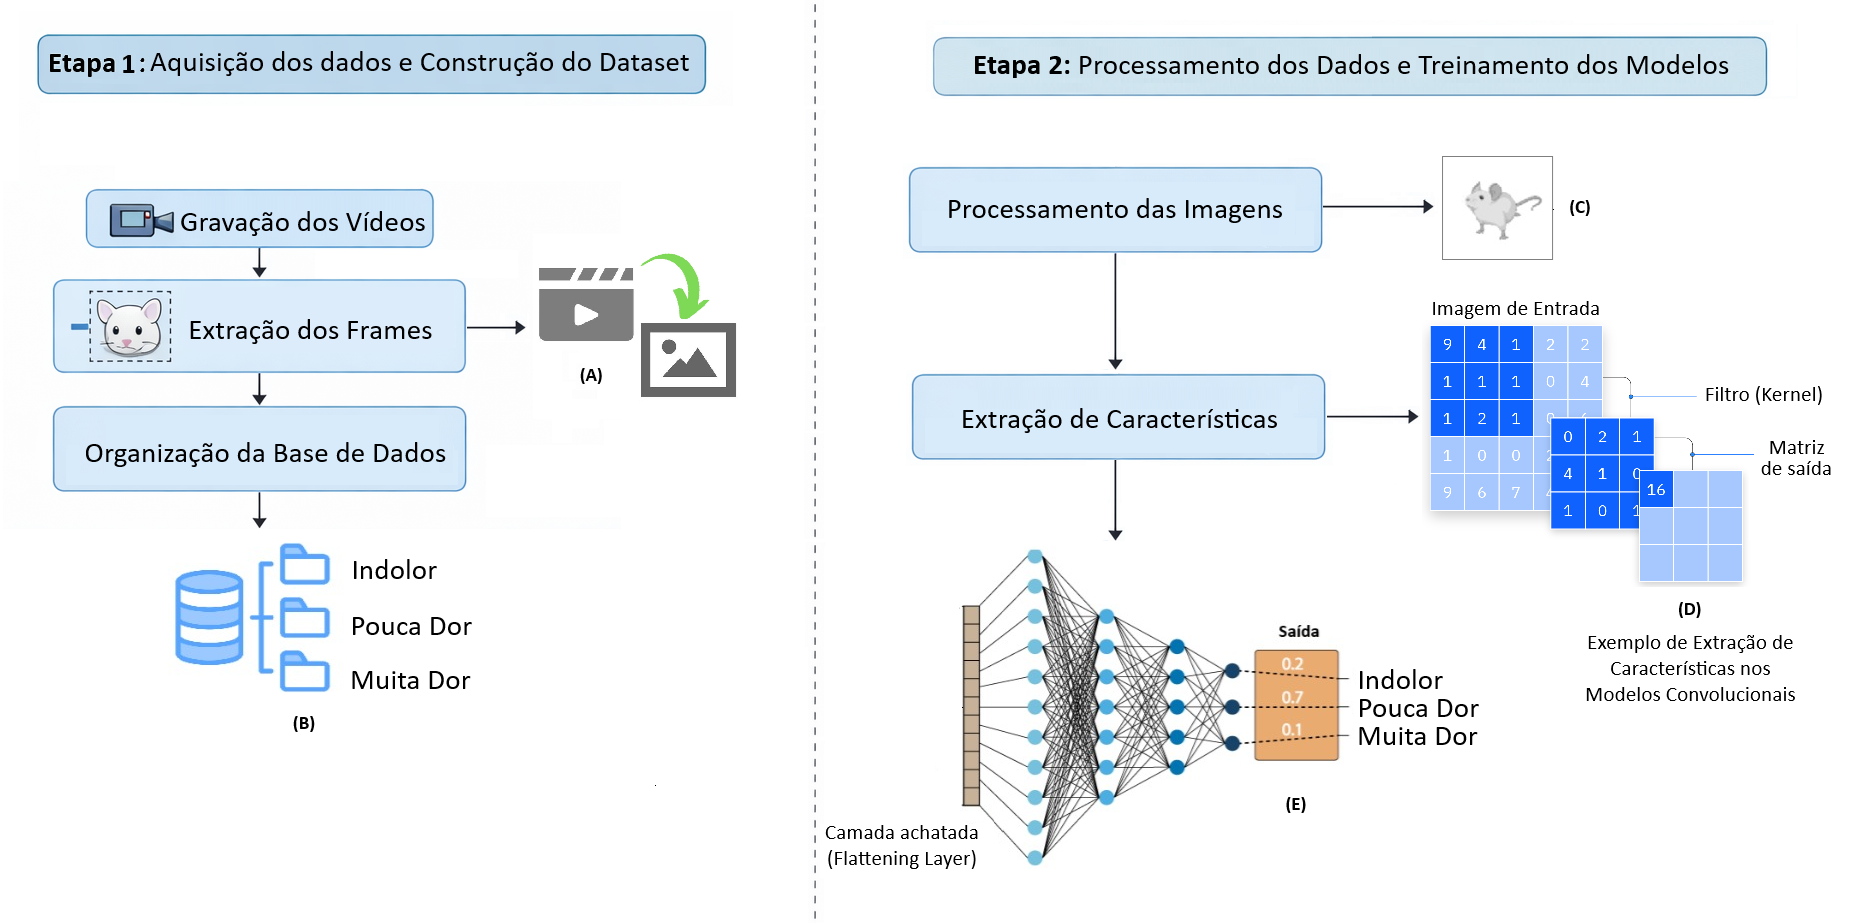
\includegraphics[width=1\linewidth]{figuras/figs_metodologia/Processo_metodologico}
	\caption{Processo metodológico adotado neste estudo. Fonte: o autor.}
	\label{fig:processometodologico}
\end{figure}

\section{Organização e Manejo dos Grupos Experimentais}

Foram utilizados camundongos da espécie \textit{Mus musculus}, modelo animal amplamente empregado em pesquisas biomédicas devido a extensa documentação genética, fisiológica e comportamental disponível na literatura, além de fatores práticos como a alta taxa reprodutiva e facilidade de manejo \cite{Bryda2013}. A amostra foi composta por animais de ambos os sexos, visando aumentar a variabilidade biológica representada no conjunto de dados e minimizar possíveis vieses amostrais. 

Optou-se pela utilização de camundongos isogênicos da linhagem BALB/c em razão de dois fatores principais: (i) a elevada homogeneidade genética característica dos animais isogênicos, reduzindo variabilidades biológicas intragrupo e favorecendo maior controle experimental; e (ii) a coloração clara da pelagem, que proporciona melhor contraste das estruturas faciais nas gravações em vídeo. Esse aspecto é particularmente relevante para a identificação visual de regiões como olhos, orelhas, focinho e vibrissas, facilitando tanto o processo de rotulagem manual quanto a extração automatizada de características associadas às unidades de ação facial descritas pela \acs{MGS}.

Os animais foram alojados em mini-isoladores apropriados, com condições ambientais rigidamente controladas, a fim de minimizar fatores externos capazes de interferir no comportamento espontâneo ou nas expressões faciais. Os camundongos foram mantidos sob ciclo claro/escuro de 12 horas, em ambiente com temperatura controlada (22°C ± 2°C) e umidade relativa de 55\% ± 5\%. A ventilação dos mini-isoladores ocorreu por meio de sistema com filtragem \acs{HEPA}, reduzindo a exposição à agentes externos e contribuindo para maior estabilidade sanitária.

Cada unidade experimental acomodou no máximo cinco animais, respeitando as recomendações institucionais de bem-estar animal e evitando superlotação. Após o período de adaptação ao ambiente experimental, os animais foram distribuídos em dois grupos principais: grupo controle (sem indução de dor) e grupo experimental (submetido ao protocolo de indução nociceptiva). 

As gravações do grupo controle foram utilizadas para caracterizar o padrão basal das expressões faciais. Já as gravações do grupo experimental forneceram amostras visuais das alterações faciais associadas ao estímulo nociceptivo em diferentes momentos temporais, permitindo registrar variações dinâmicas da intensidade de dor ao longo do experimento.

A definição clara das classes e o controle das variáveis experimentais constituem etapas fundamentais para reduzir ruídos no treinamento dos modelos e aumentar a confiabilidade das análises realizadas. Além disso, a estruturação dos grupos permitiu a obtenção de dados longitudinais das expressões faciais, ampliando o potencial exploratório da base de dados e favorecendo o desenvolvimento de modelos mais sensíveis às variações sutis associadas aos diferentes estados fisiológicos avaliados.

\section{Protocolo para Indução de Dor}

Os camundongos pertencentes ao grupo experimental foram submetidos ao modelo clássico de indução da dor via formalina descrito por \cite{Langford2010}. Esse modelo é reconhecido por sua robustez experimental e por produzir respostas fisiológicas e comportamentais previsíveis, tornando-se adequado para investigações envolvendo análise temporal da dor.

O procedimento consiste na administração subcutânea de 20$\mu$L da solução de formalina a 5\% na região plantar da pata traseira direita e produz uma resposta bifásica temporalmente bem definida. Inicialmente, ocorre uma fase aguda (0–15 minutos), correspondente à resposta imediata ao estímulo químico e geralmente associada a maior intensidade dolorosa. Em seguida, desenvolve-se uma segunda fase (15–30 minutos), caracterizada pela manutenção do quadro doloroso em decorrência da ativação de mecanismos inflamatórios locais.

Imediatamente após a aplicação da formalina, os animais foram posicionados nas caixas de observação previamente preparadas para registro em vídeo. As filmagens tiveram início logo após o procedimento, garantindo o registro das alterações faciais correspondentes às fases iniciais do estímulo nociceptivo. Decorridos 30 minutos da injeção, os animais receberam analgesia com sulfato de morfina (5 a 10 mg/kg), administrado por via subcutânea, conforme descrito pela Figura \ref{fig:protocolo}. 

\begin{figure}[h]
	\centering
	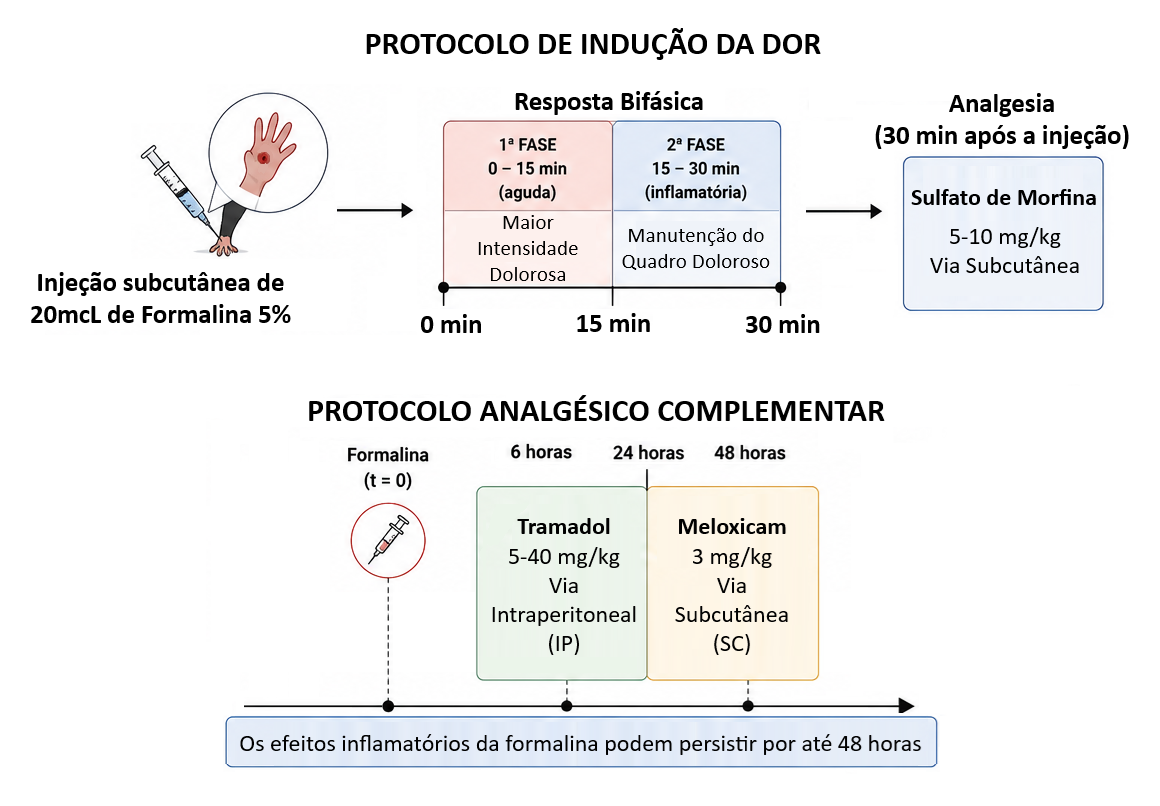
\includegraphics[width=1\linewidth]{figuras/figs_metodologia/langford}
	\caption{Diagrama visual do protocolos experimentais descritos por Langford e Wjeeler-Aceto. Fonte: o autor.}
	\label{fig:protocolo}
\end{figure}

Considerando que os efeitos inflamatórios induzidos pela formalina podem persistir por até 48 horas \cite{WheelerAceto1990}, foi estabelecido um protocolo complementar de controle analgésico e anti-inflamatório. Seis horas após o procedimento inicial, administrou-se cloridrato de tramadol (5–40 mg/kg, via intraperitoneal), repetido também após 24 e 48 horas. Paralelamente, os animais receberam meloxicam (3 mg/kg, via subcutânea) nos mesmos intervalos temporais, com o objetivo de auxiliar no controle do componente inflamatório associado ao procedimento, também descrito pela Figura \ref{fig:protocolo}.

Durante o período total de 72 horas de observação, os animais foram filmados sistematicamente uma hora antes e uma hora após cada administração analgésica. Essa estratégia experimental permitiu registrar diferentes condições fisiológicas: (i) estado basal; (ii) dor ativa sem intervenção imediata; e (iii) dor sob efeito farmacológico. Ao término do período experimental, todos os animais foram submetidos à eutanásia humanitária mediante anestesia profunda com associação de cetamina e xilazina (via intraperitoneal), seguida de deslocamento cervical como método complementar para confirmação do óbito. Todos os procedimentos foram previamente aprovados pelo \ac{CEUA}, em conformidade com as diretrizes do Conselho Nacional de Controle de Experimentação Animal (\acs{CONCEA}/\acs{MCTI}), sob protocolo \textit{\acs{CONCEA}/\acs{MCTI}/0301052024/PESQUISA/000000/2025}.

\section{Aquisição da Base de Dados}

As gravações de ambos os grupos experimentais foram realizadas em alta resolução (4K, 60 quadros por segundo) utilizando câmeras digitais de \textit{smartphones} (modelo \textit{iPhone 13}) previamente higienizados e posicionados frontalmente às caixas de observação. O enquadramento foi ajustado para maximizar a visibilidade dos animais, mantendo distância e ângulo constantes ao longo das sessões.

Cada isolador contendo os camundongos foi filmado durante dois minutos, totalizando 15 repetições por sessão, com intervalos de um minuto entre cada gravação. Esse procedimento foi aplicado tanto antes quanto após o protocolo da indução de dor, assegurando equilíbrio temporal entre as coletas das condições basal e experimental, conforme ilustrado na Figura \ref{fig:capturaimagens}. 

\begin{figure}[h]
	\centering
	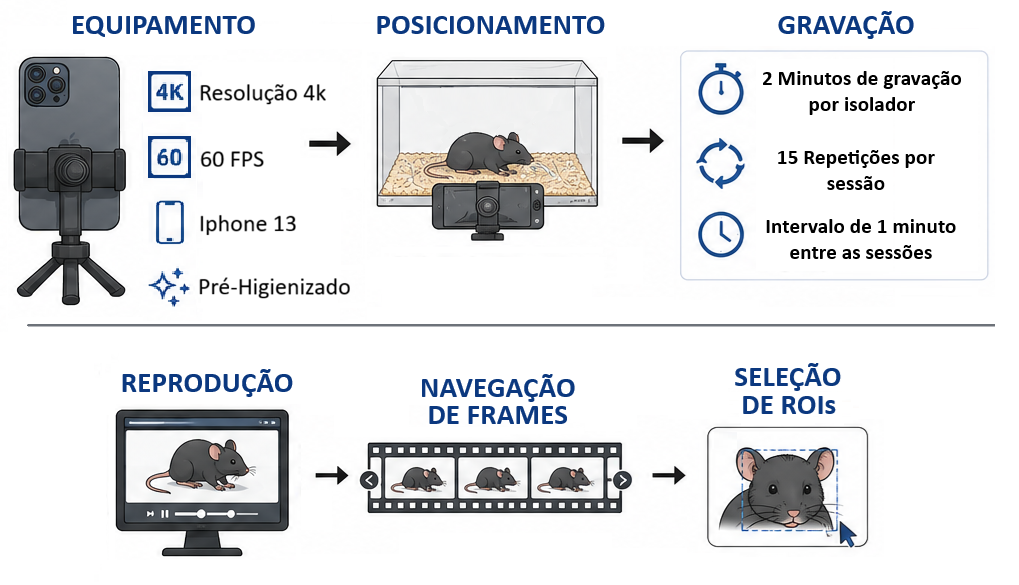
\includegraphics[width=1\linewidth]{figuras/figs_metodologia/captura}
	\caption{Processo de captura dos vídeos para a construção da base de dados. Fonte: Imagem gerada por inteligência artificial (\textit{ChatGPT - OpenAI}), elaborada pelo autor.}
	\label{fig:capturaimagens}
\end{figure}

Após a etapa de captura, os vídeos foram processados por meio de um software desenvolvido especificamente para este estudo, projetado para permitir reprodução controlada dos vídeos, navegação quadro a quadro e seleção manual das regiões de interesse (\acsp{ROI}). Cada imagem extraída foi associada a um identificador único, evitando redundâncias e facilitando o rastreamento posterior das amostras.

Importante destacar que a ferramenta desenvolvida para a extração dos quadros possui um sistema de controle automatizado do armazenamento, o qual impede a duplicidade de imagens na base, além de fornecer ferramentas extras para a inspeção visual e exclusão controlada de quadros inconsistentes ou inadequadas para análise.

Cada imagem selecionada foi inicialmente rotulada em uma das quatro categorias previamente definidas: \textit{Indolor}, \textit{Pouca Dor}, \textit{Muita Dor} ou \textit{Incerto}. A categoria \textit{Incerto} foi utilizada apenas durante o processo inicial de triagem para lidar com imagens ambíguas ou de difícil classificação. 

O software desenvolvido foi disponibilizado à equipe veterinária responsável pela etapa de coleta e rotulagem dos dados. Especialistas com experiência em avaliação de dor em camundongos realizaram a análise visual das imagens utilizando como referência os critérios estabelecidos pela \acs{MGS}. Esse procedimento colaborativo contribuiu para aumentar a confiabilidade da rotulagem e reduzir possíveis vieses individuais.

\section{Seleção das Arquiteturas de Classificação}

A escolha da arquitetura de classificação constitui uma etapa fundamental no desenvolvimento de sistemas computacionais aplicados à análise de imagens. A definição do modelo impacta diretamente as tarefas supervisionadas de classificação dos padrões visuais, influenciando aspectos como desempenho preditivo, estabilidade do treinamento, capacidade de generalização e custo computacional.

Com o objetivo de fundamentar essa escolha de forma criteriosa, foi conduzida uma revisão da literatura especializada envolvendo trabalhos clássicos e recentes nas áreas de aprendizado profundo, reconhecimento facial e classificação de imagens. Os principais critérios considerados para seleção das arquiteturas incluíram: (i) desempenho reportado na literatura; (ii) eficiência computacional; (iii) capacidade de aprendizado e generalização; e (iv) potencial de aplicação em cenários com restrições computacionais.

Dentre as arquiteturas selecionadas, destacam-se inicialmente os modelos baseados em Redes Neurais Convolucionais (\acsp{CNN}), amplamente consolidados em tarefas de visão computacional devido à elevada capacidade de extração automática das características espaciais.

A família de arquiteturas \textit{ResNet} foi incluída neste estudo em razão de seu desempenho amplamente validado em \textit{benchmarks} de larga escala, como o \textit{ImageNet}. Seu principal diferencial está na incorporação do aprendizado residual, permitindo o treinamento de redes profundas com maior estabilidade e reduzindo problemas associados ao desaparecimento do gradiente. Além disso, sua estrutura modular possibilita a utilização de variantes com diferentes profundidades, tornando a arquitetura flexível para distintos cenários computacionais.

Outra arquitetura baseada em \acs{CNN} considerada neste trabalho foi a \textit{DenseNet}, caracterizada pelo padrão de conectividade densa entre suas camadas. Nesse modelo, cada camada recebe como entrada os mapas de características produzidos por todas as camadas anteriores dentro do mesmo bloco, promovendo reaproveitamento contínuo das informações ao longo da rede. Em problemas que envolvem padrões visuais sutis — como os indicadores faciais associados à \acs{MGS} —, essa capacidade de preservação e combinação de informações em diferentes níveis de abstração pode favorecer a construção de representações mais discriminativas.

A arquitetura \textit{MobileNet} também foi selecionada devido à sua elevada eficiência computacional, sendo projetada especificamente para aplicações com restrições de processamento. Seu principal diferencial consiste na utilização de convoluções separáveis em profundidade, reduzindo significativamente o número de parâmetros e o custo computacional sem comprometer substancialmente o desempenho. Além disso, mecanismos como o \textit{width multiplier} e o \textit{resolution multiplier} permitem ajustar diretamente o equilíbrio entre desempenho e complexidade computacional, ampliando o potencial de aplicação em dispositivos móveis e sistemas embarcados.

Além das arquiteturas convolucionais tradicionais, este estudo também investigou abordagens baseadas em mecanismos de atenção por meio da arquitetura \textit{Vision Transformer} (\acs{VIT}). Diferentemente das \acsp{CNN}, o \acs{VIT} processa imagens utilizando mecanismos de autoatenção, possibilitando modelar dependências globais entre diferentes regiões da imagem desde as etapas iniciais do treinamento.

A adoção do \acs{VIT} foi motivada pela capacidade de capturar relações de longo alcance entre diferentes regiões faciais, potencialmente favorecendo representações mais abrangentes dos padrões associados à dor. Essa característica torna a arquitetura particularmente interessante em problemas envolvendo variações sutis nas expressões faciais, nos quais relações espaciais globais podem desempenhar papel relevante na discriminação entre diferentes níveis de dor.

Entretanto, diferentemente das arquiteturas convolucionais, modelos baseados em \textit{Transformers} tendem a demandar maior volume de dados para treinamento eficiente, uma vez que não incorporam explicitamente os vieses indutivos locais característicos das \acsp{CNN}. Dessa forma, sua inclusão neste estudo também permitiu investigar o impacto dessas diferenças estruturais em cenários associados ao uso de \textit{transfer learning}.

A seleção conjunta dessas arquiteturas possibilitou estabelecer uma análise comparativa entre modelos baseados em diferentes paradigmas de aprendizado visual, permitindo investigar não apenas o desempenho preditivo, mas também características relacionadas à eficiência computacional, capacidade de generalização e adequação ao problema proposto.

\section{Configuração Experimental}

Em problemas relacionados ao aprendizado supervisionado, pequenas variações na organização das amostras, nos procedimentos de pré-processamento ou na divisão entre os conjuntos de treinamento e validação podem influenciar significativamente os resultados obtidos, comprometendo a reprodutibilidade e a comparabilidade dos experimentos. Portanto, a seguinte seção tem como objetivo descrever as configurações utilizadas para o processamento dos dados, bem como condução metodológica dos experimentos.

Visando promover a transparência científica e favorecer a reprodução dos experimentos conduzidos nesta pesquisa, todos os recursos desenvolvidos foram disponibilizados publicamente por meio de repositórios digitais. Em particular, foram compartilhados: (i) o código-fonte da ferramenta desenvolvida para a extração, organização e gerenciamento da base de dados; (ii) o projeto contendo a implementação dos modelos de aprendizado profundo, bem como as rotinas de treinamento, validação e avaliação experimental; e (iii) a base de dados construída e utilizada ao longo deste trabalho. Todos esses recursos encontram-se disponíveis no repositório oficial do autor, acessível em:

\begin{itemize}
	
	\item Ferramenta para geração da base de dados:\\
	\url{https://github.com/Marcio-Salmazo/Projeto-video-player}
	
	\item Implementação dos modelos classificadores:\\
	\url{https://github.com/Marcio-Salmazo/Projeto-Classificadores}
	
	\item Base de dados utilizada nesta pesquisa:\\
	\url{https://github.com/Marcio-Salmazo/Dataset-MGS}
	
\end{itemize}

\subsection*{Preparação da Base de Dados}

O controle sobre a preparação da base de dados foi aplicado por meio de um \textit{Script} em \textit{python}, desenvolvido para gerenciar a separação automatizada da base em subconjuntos de treinamento e validação. O algoritmo permite definir previamente a proporção de imagens destinada a cada subconjunto, reproduzindo automaticamente a estrutura hierárquica das classes em cada diretório e preservando a integridade do conjunto original de dados.

O processo de divisão da base foi realizado de forma estratificada por classe, assegurando a manutenção proporcional das categorias entre os subconjuntos gerados. Para cada classe, o algoritmo aplica um processo de embaralhamento pseudoaleatório controlado por uma semente fixa (\textit{random seed}), garantindo reprodutibilidade experimental em diferentes execuções. Após o embaralhamento, as imagens são copiadas da base original e redistribuídas automaticamente entre os subconjuntos definidos. A estrutura final da base de dados é apresentada na Figura \ref{fig:estrutrabase}.

\begin{figure}[h]
	\centering
	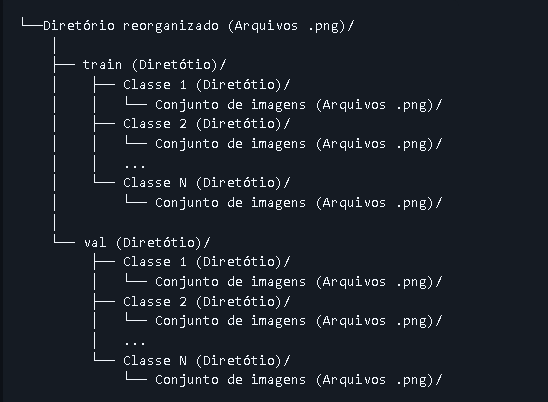
\includegraphics[width=.8\linewidth]{figuras/figs_metodologia/estrutra_base}
	\caption{Estrutura final da base de dados, após o processo de divisão dos conjuntos de treino e validação. Fonte: o autor.}
	\label{fig:estrutrabase}
\end{figure}

% TRECHO NOVO SOBRE O CARREGAMENTO DOS DADOS
\subsection*{Carregamento dos Dados}

Após a organização da base de dados, foi aplicada uma etapa de pré-processamento com o objetivo de padronizar as imagens e proporcionar condições adequadas para o treinamento das arquiteturas investigadas. Nessa etapa, foram adotadas estratégias distintas para os conjuntos de treinamento e validação, de forma a preservar as características específicas de cada etapa do processo de aprendizado.

Para o conjunto de treinamento, empregou-se uma estratégia de \textit{data augmentation} leve, baseada em pequenas transformações geométricas e espaciais realizadas de forma aleatória. Essas modificações tiveram como finalidade ampliar artificialmente a variabilidade das amostras disponíveis, expondo os modelos a diferentes representações de uma mesma imagem sem alterar as características faciais associadas à expressão de dor. Essa abordagem contribui para a capacidade de generalização dos classificadores diante de pequenas variações presentes durante a aquisição das imagens.

Em contrapartida, o conjunto de validação foi submetido apenas a operações de padronização, sem a aplicação de transformações aleatórias. Essa estratégia garante que o desempenho dos modelos seja avaliado de maneira consistente ao longo do treinamento, permitindo comparações imparciais entre as diferentes arquiteturas investigadas. Por fim, todas as imagens foram normalizadas antes de serem utilizadas pelos modelos, assegurando uma representação padronizada dos dados e contribuindo para a estabilidade do processo de treinamento.

\subsection*{Métricas para Avaliação do Desempenho}

Durante o treino, métricas primárias como função de perda (\textit{loss}) e acurácia (\textit{accuracy}) foram registradas automaticamente ao final de cada época por meio dos mecanismos de \textit{log} integrados ao \textit{TensorFlow} e às rotinas implementadas em ambiente \textit{JAX/Flax}. Esses registros foram armazenados em arquivos nos formatos \textit{.csv} e \textit{.xlsx}, possibilitando posterior organização, consolidação e análise dos resultados obtidos.

A acurácia foi utilizada como principal indicador de desempenho dos classificadores por representar a proporção de amostras corretamente classificadas em relação ao total avaliado. Considerando que o objetivo central deste estudo consiste na comparação da capacidade de diferentes arquiteturas neurais em identificar padrões faciais associados à dor, a acurácia fornece uma medida direta e intuitiva da eficiência global dos modelos. 

De modo complementar, a função de perda foi utilizada como principal métrica para acompanhamento do processo de otimização durante o treinamento. Diferentemente da acurácia, a função de perda quantifica o grau de erro cometido pelo modelo em suas predições, considerando também o nível de confiança associado às decisões produzidas. Dessa forma, reduções sucessivas nos valores de perda indicam que o modelo está ajustando seus parâmetros internos de maneira consistente, aproximando suas previsões dos rótulos esperados e favorecendo o processo de convergência.

Embora a literatura apresente diversas métricas complementares para avaliação de classificadores, tais como precisão, sensibilidade (\textit{recall}), \textit{F1-score} e matrizes de confusão, sua utilização não foi considerada necessária para os objetivos deste estudo. Como a pesquisa teve como foco principal a análise comparativa da eficiência de diferentes arquiteturas de aprendizado profundo, priorizou-se a utilização de métricas capazes de representar diretamente o desempenho global e a dinâmica de aprendizado dos modelos. Dessa forma, acurácia e função de perda mostraram-se suficientes para sustentar as análises realizadas e responder às questões de pesquisa propostas.

% TRECHO NOVO SOBRE O DETALHAMENTO DE HARDWARE
\subsection*{Detalhamento de Hardware}

Os experimentos conduzidos nesta pesquisa foram realizados em dois ambientes computacionais distintos, de acordo com as exigências de processamento de cada arquitetura investigada. Os treinamentos envolvendo as arquiteturas convolucionais foram executados em uma estação de trabalho pessoal equipada com processador \textit{AMD Ryzen 7 5700X}, 24 GB de memória \textit{RAM} e uma unidade de processamento gráfico (GPU) \textit{NVIDIA GeForce RTX 3070}. Cabe destacar que os modelos avaliados apresentam complexidade computacional compatível com a capacidade de processamento e memória disponibilizadas pela GPU.

Por outro lado, os experimentos envolvendo a arquitetura \acs{VIT} foram conduzidos em um servidor remoto pertencente à Universidade Federal de Uberlândia (UFU), acessado por meio do protocolo SSH. O servidor utilizado foi equipada com processador \textit{Intel Xeon Gold 6426Y}, 256 GB de memória \textit{RAM} e uma GPU \textit{NVIDIA Ampere A40}, com 48GB de \textit{VRAM}. A utilização dessa infraestrutura foi necessária ao maior custo computacional associado aos mecanismos de autoatenção empregados pelos modelos baseados em \textit{Transformers}, os quais apresentam maior consumo de memória e maior tempo de processamento durante o treinamento, mesmo com a utilização de \textit{transfer learning} para reduzir a demanda por recursos computacionais.


% ----------------------------------------------------------
% Experimentos e avaliação dos resultados
% ----------------------------------------------------------
\chapter[Experimentos e Análise dos Resultados]{Experimentos e Análise dos Resultados}

Nesta seção, são apresentados os experimentos conduzidos para avaliar o desempenho dos modelos de classificação propostos para a detecção automática de dor com base na \textit{Mouse Grimace Scale}, bem como para investigar o impacto de diferentes escolhas de modelagem na capacidade de generalização dos classificadores.

Com o objetivo de garantir a comparabilidade entre os resultados, os modelos avaliados foram padronizados quanto aos parâmetros de entrada e à forma de distribuição dos dados. Essa padronização minimiza a influência de variações na amostragem e permite que as diferenças de desempenho observadas sejam atribuídas, predominantemente, às características estruturais e ao comportamento de aprendizado das arquiteturas analisadas.

O procedimento experimental foi estruturado em três etapas principais, organizadas de forma progressiva. Na etapa inicial, buscou-se verificar a capacidade dos modelos de aprender padrões a partir dos dados. Essa avaliação foi realizada por meio do monitoramento da redução da função de perda ao longo do treinamento, indicando o correto funcionamento do pipeline de processamento e dos mecanismos de otimização. Essa fase foi conduzida em condições controladas, utilizando um subconjunto reduzido de dados, com foco na validação do pipeline, e não no desempenho absoluto dos modelos.

Na segunda etapa, foi realizada a exploração dos hiperparâmetros, com o objetivo de identificar configurações mais adequadas para cada arquitetura. Os experimentos foram conduzidos em escala intermediária, utilizando o conjunto de dados completo e ampliando gradualmente as épocas de treinamento, bem como a complexidade em relação à fase anterior. Adicionalmente, foram analisadas as curvas de aprendizado, permitindo avaliar a estabilidade do processo de treinamento e identificar possíveis indícios de \textit{overfitting} (sobreajuste) ou \textit{underfitting} (subajuste).

Por fim, na terceira etapa, os modelos foram treinados com foco na maximização da capacidade de generalização. O número de épocas foi definido com base na estabilização das métricas de validação, bem como na identificação de platôs de desempenho ao longo do treinamento. As seções subsequentes apresentam uma descrição detalhada dos cenários experimentais considerados, incluindo as configurações adotadas e uma análise crítica dos resultados obtidos.

\section{Experimento 1 - Implementação e Validação dos Modelos Selecionados}

O primeiro experimento teve como finalidade implementar e validar a operação dos modelos selecionados neste estudo, assegurando que sua construção esteja consistente com as especificações descritas na literatura original. Para isso, foram consideradas como referência as propostas de \cite{he2016} para os modelos da família \textit{ResNet}, \cite{Howard2017} para a arquitetura \textit{MobileNet}, \cite{Huang2017} para a \textit{DenseNet} e \cite{dosovitskiy2020vit} para a arquitetura \textit{Vision Transformer} (\acs{VIT}).

Este experimento atua como uma etapa de validação preliminar, viabilizando a identificação precoce de possíveis inconsistências, tais como falhas no carregamento e processamento dos dados, instabilidades numéricas durante o treinamento (como explosão ou desaparecimento do gradiente), erros no cálculo e registro das métricas, bem como comportamentos anômalos das arquiteturas. Nesse contexto, o objetivo não foi avaliar o desempenho absoluto dos modelos, mas verificar sua capacidade de aprender a partir dos dados e apresentar comportamento consistente durante o processo de otimização.

Para isso, o treinamento foi executado utilizando um subconjunto reduzido da base de dados e um número limitado de épocas. A validação foi considerada satisfatória quando observada uma tendência de convergência, evidenciada pela redução progressiva da função de perda e pelo aumento da acurácia ao longo do treinamento. Dessa forma, foi possível obter evidências de que os componentes responsáveis pelo carregamento dos dados, propagação direta, retropropagação dos gradientes e atualização dos parâmetros estavam operando corretamente.

\subsection{Modelos da Arquitetura \textit{ResNet}}

O trabalho de \cite{he2016} apresenta a configuração estrutural de diferentes variantes da arquitetura \textit{ResNet}, que se distinguem principalmente pela profundidade da rede. No contexto deste estudo, a seleção dos modelos considerou as o tamanho reduzido do conjunto de dados e a baixa complexidade de classificação da tarefa proposta, optando-se por arquiteturas de menor e média profundidade.

Dessa forma, foram selecionadas as variantes \textit{ResNet-18}, \textit{ResNet-34} e \textit{ResNet-50}, por apresentarem um equilíbrio adequado entre capacidade de representação e custo computacional. A organização estrutural desses modelos segue as especificações descritas na literatura original, conforme apresentado na Tabela \ref{tab:resnet_variants_structure}.

\begin{table}[h]
	\centering
	\caption{Comparação estrutural dos diferentes modelos variantes da arquitetura \textit{ResNet}.}
	\label{tab:resnet_variants_structure}
	\renewcommand{\arraystretch}{1.1}
	
	\resizebox{\textwidth}{!}{
	\begin{tabular}{l|c|c|c|c}
		
		\toprule
		\textbf{Camada} & \textbf{ResNet-10} & \textbf{ResNet-18} & \textbf{ResNet-34} & \textbf{ResNet-50} \\
		
		\midrule
		
		Conv1 
		& \multicolumn{4}{c}{$7 \times 7$, 64, stride 2, output: $112 \times 112$} \\
		
		MaxPool 
		& \multicolumn{4}{c}{$3 \times 3$, stride 2, output: $56 \times 56$} \\
		
		\hline
		
		Conv2\_x 
		& $\left[\begin{array}{l} 3\times3, 64 \\ 3\times3, 64 \end{array}\right] \times 1$
		& $\left[\begin{array}{l} 3\times3, 64 \\ 3\times3, 64 \end{array}\right] \times 2$
		& $\left[\begin{array}{l} 3\times3, 64 \\ 3\times3, 64 \end{array}\right] \times 3$
		& $\left[\begin{array}{l} 1\times1, 64 \\ 3\times3, 64 \\ 1\times1, 256 \end{array}\right] \times 3$ \\
		
		\hline
		
		Output size 
		& \multicolumn{4}{c}{$56 \times 56$} \\
		
		\hline
		
		Conv3\_x 
		& $\left[\begin{array}{l} 3\times3, 128 \\ 3\times3, 128 \end{array}\right] \times 1$
		& $\left[\begin{array}{l} 3\times3, 128 \\ 3\times3, 128 \end{array}\right] \times 2$
		& $\left[\begin{array}{l} 3\times3, 128 \\ 3\times3, 128 \end{array}\right] \times 4$
		& $\left[\begin{array}{l} 1\times1, 128 \\ 3\times3, 128 \\ 1\times1, 512 \end{array}\right] \times 4$ \\
		
		\hline
		
		Output size 
		& \multicolumn{4}{c}{$28 \times 28$} \\
		
		\hline
		
		Conv4\_x 
		& $\left[\begin{array}{l} 3\times3, 256 \\ 3\times3, 256 \end{array}\right] \times 1$
		& $\left[\begin{array}{l} 3\times3, 256 \\ 3\times3, 256 \end{array}\right] \times 2$
		& $\left[\begin{array}{l} 3\times3, 256 \\ 3\times3, 256 \end{array}\right] \times 6$
		& $\left[\begin{array}{l} 1\times1, 256 \\ 3\times3, 256 \\ 1\times1, 1024 \end{array}\right] \times 6$ \\
		
		\hline
		
		Output size 
		& \multicolumn{4}{c}{$14 \times 14$} \\
		
		\hline
		
		Conv5\_x 
		& $\left[\begin{array}{l} 3\times3, 512 \\ 3\times3, 512 \end{array}\right] \times 1$
		& $\left[\begin{array}{l} 3\times3, 512 \\ 3\times3, 512 \end{array}\right] \times 2$
		& $\left[\begin{array}{l} 3\times3, 512 \\ 3\times3, 512 \end{array}\right] \times 3$
		& $\left[\begin{array}{l} 1\times1, 512 \\ 3\times3, 512 \\ 1\times1, 2048 \end{array}\right] \times 3$ \\
		
		\hline
		
		Output size 
		& \multicolumn{4}{c}{$7 \times 7$} \\
		
		\hline
		
		AvgPool 
		& \multicolumn{4}{c}{Global average pooling ($1 \times 1$)} \\
		
		FC 
		& \multicolumn{4}{c}{Fully connected layer (3 classes)} \\
		
		\bottomrule
	\end{tabular}
	}
	
\end{table}

O modelo \textit{ResNet-10} corresponde a uma variação ainda mais simplificada da arquitetura proposta por \cite{he2016}, embora não tenha sido originalmente apresentada no artigo, ela permitem avaliar se uma redução adicional da complexidade estrutural pode resultar em treinamento mais estável ou melhor capacidade de generalização em cenários caracterizados por conjuntos de dados limitados, justificando sua adoção para este experimento.
 
Essa variante é composta por dez camadas convolucionais e mantém o mesmo princípio estrutural de aprendizado residual e organização modular baseada em \textit{basic blocks} presente nas demais arquiteturas rasas da família \textit{ResNet} — como as variantes \textit{ResNet-18} e \textit{ResNet-34} — diferenciando-se principalmente no número de blocos e, consequentemente, na profundidade total da rede, conforme ilustrado pela Tabela \ref{tab:resnet_variants_structure}.

Para garantir maior fidelidade ao estudo de \cite{he2016}, o treinamento foi conduzido, sempre que possível, seguindo as configurações de parâmetros descritas no trabalho original, sendo realizadas adaptações apenas nos casos em que tais configurações se mostraram incompatíveis com o cenário experimental definido neste projeto.

No que se refere ao pré-processamento dos dados, buscou-se reproduzir o pipeline adotado pelos autores. Inicialmente, as imagens foram redimensionadas de modo que o menor lado fosse amostrado aleatoriamente no intervalo de [256, 480]. Em seguida, foi aplicada uma operação de \textit{random crop} com tamanho fixo de 224×224 \textit{pixels}, acompanhada de espelhamento horizontal aleatório. Por fim, realizou-se a normalização dos dados de entrada de forma canal a canal, utilizando a média e o desvio padrão calculados a partir do conjunto \textit{ImageNet}.

Adicionalmente, conforme descrito em \cite{he2016}, foi empregada a técnica de \textit{Batch Normalization} (\acs{BN}) após cada camada convolucional e antes da aplicação da função de ativação \textit{\acs{ReLU}}. No trabalho original - implementado no \textit{framework} \textit{Caffe} \cite{jia2014caffe} -, a \acs{BN} é definida como uma camada específica, frequentemente acompanhada por uma camada adicional denominada \textit{Scale}, responsável por aplicar os parâmetros aprendíveis de escala e deslocamento. O processo de normalização pode ser descrito pela seguinte expressão:

\begin{equation}
	x_{norm} = \frac{x - \mu}{\sigma}
\end{equation}

$\mu$ e $\sigma$ correspondem, respectivamente, à média e ao desvio padrão estimados para cada canal. Essa normalização tem como objetivo padronizar a distribuição dos dados de entrada, contribuindo para a estabilidade do treinamento.

No contexto deste trabalho, a implementação foi realizada utilizando o \textit{TensorFlow}, no qual a camada \textit{Batch Normalization} já incorpora internamente os parâmetros de escala e deslocamento, além de gerenciar automaticamente as estatísticas necessárias durante as fases de treinamento e inferência. Essa diferença de implementação não altera o princípio fundamental da técnica, mas simplifica sua utilização prática.

Os autores de \cite{he2016} também destacam a não utilização de \textit{dropout}, uma vez que a \textit{Batch Normalization} já exerce um efeito regularizador significativo. Neste experimento o treinamento foi conduzido por um total de 10 épocas, utilizando a base de dados com imagens dos camundongos, além disso, o \textit{batch size} precisou ser reduzido de 256 para 32 considerando limitações de hardware, tamanho da base utilizada e complexidade do problema. O resultado é descrito na Tabela \ref{tab:resnet_sanity_unified}.

% VALORES OBTIDOS DOS EXPERIMENTOS 14,15 e 16 
\begin{table}[h]
	\centering
	\caption{Valores resultantes para cada modelo variante da arquitetura \textit{ResNet}, durante o teste de validação inicial. Importante ressaltar que o objetivo não foi avaliar o desempenho absoluto dos modelos, mas sim, sua tendência de aprendizado.}
	\begin{tabular}{c|cc|cc|cc}
		
		\toprule
		\multirow{2}{*}{\textbf{Época}} 
		& \multicolumn{2}{c|}{\textbf{ResNet-18}} 
		& \multicolumn{2}{c|}{\textbf{ResNet-34}} 
		& \multicolumn{2}{c}{\textbf{ResNet-50}} \\
		
		& Acurácia & Perda & Acurácia & Perda & Acurácia & Perda \\
		
		\midrule
		
		1  & 0.4420 & 1.4406 & 0.4480 & 1.8220 & 0.4456 & 2.8179 \\
		3  & 0.4481 & 1.4252 & 0.4528 & 1.7870 & 0.4788 & 2.7549 \\
		5  & 0.4511 & 1.4145 & 0.4619 & 1.7630 & 0.5007 & 2.6919 \\
		7  & 0.4760 & 1.3939 & 0.4651 & 1.7384 & 0.5221 & 2.6262 \\
		9  & 0.4982 & 1.3735 & 0.4805 & 1.7143 & 0.5172 & 2.5747 \\
		\bottomrule
	\end{tabular}
	\label{tab:resnet_sanity_unified}
\end{table}

Observa-se nos resultados, um comportamento caracterizado pela redução progressiva da função de perda (\textit{loss}) e pelo aumento gradual da acurácia ao longo das épocas. Esse padrão indica uma capacidade consistente de aprendizado, evidenciando o correto funcionamento do pipeline de treinamento, incluindo as etapas de carregamento e pré-processamento dos dados, bem como os mecanismos de otimização empregados. 

Adicionalmente, não foram observadas instabilidades significativas, como explosão ou desaparecimento do gradiente, nem oscilações anômalas nas métricas monitoradas. Embora os valores absolutos de desempenho ainda sejam modestos — o que é esperado, dado o uso de número limitado de épocas —, a tendência consistente de melhoria nas métricas confirma que as arquiteturas estão operando conforme o esperado.

\subsection{Arquiteturas \textit{MobileNet} e \textit{DenseNet}}

Ambas as arquiteturas convolucionais \textit{MobileNet} e \textit{DenseNet} seguiram o mesmo protocolo de validação adotado para a arquitetura \textit{ResNet}. O objetivo desta etapa do experimento permanece o mesmo: permitir a identificação precoce de possíveis inconsistências, instabilidades numéricas ou comportamentos anômalos dos modelos ao longo das 10 épocas de treinamento.

A configuração dos parâmetros buscou, sempre que possível, manter-se alinhada aos trabalhos originais propostos por \cite{Howard2017} e \cite{Huang2017}. No entanto, foram realizadas adaptações específicas, incluindo a redução da resolução de entrada das imagens, a diminuição do tamanho do \textit{batch} e o ajuste da taxa de aprendizado, com o objetivo de tornar o treinamento mais estável e adequado ao cenário experimental deste projeto. A Tabela \ref{tab:unified_training_config} apresenta, os valores dos parâmetros utilizados no experimento.

Apesar dessas modificações, os elementos estruturais fundamentais das arquiteturas foram preservados. Em particular, destacam-se o uso de convoluções separáveis em profundidade na \textit{MobileNet} e o padrão de conectividade densa na \textit{DenseNet}, caracterizado pela taxa de crescimento ($k$) e pelo fator de compressão ($\theta$). A manutenção desses componentes assegura a compatibilidade conceitual aos modelos propostos na literatura.

\begin{table}[h]
	\centering
	\caption{Configuração estrutural dos modelos MobileNet-V1 e DenseNet.}
	\label{tab:unified_training_config}
	\renewcommand{\arraystretch}{1.3}
	
	\begin{tabular}{l | c | c}
		
		\toprule
		\textbf{Parâmetro} & \textbf{DenseNet} & \textbf{MobileNet}\\
		\midrule
		
		Arquitetura / Estrutura 
		& [6, 8, 12, 8] (Blocos Densos) 
		& MobileNet-V1\\
		
		Input size 
		& $128 \times 128 \times 3$ 
		& $160 \times 160 \times 3$\\
		
		\hline
		\makecell[l]{Divisão para o\\conjunto de validação}
		& \multicolumn{2}{c}{0.20} \\
		
		\hline
		
		Função Perda
		& Sparse Categorical CE 
		& Sparse Categorical CE\\
		
		Otimizador 
		& SGD (Nesterov) 
		& RMSprop\\
		
		\textit{Learning Rate} Inicial 
		& $1 \times 10^{-2}$ 
		& $1 \times 10^{-3}$\\
		
		\hline
		
		\textit{Momentum} 
		& \multicolumn{2}{c}{0.9} \\
		
		\hline
		
		\textit{Batch size }
		& 32 
		& 32\\
		
		\hline
		
		Critério de parada
		& \multicolumn{2}{c}{Estabilização no conjunto de validação}\\
		
		\hline
		
		\textit{Hardware} 
		& \multicolumn{2}{c}{Aceleração por GPU  (RTX-3070)}\\
		
		\hline
		
		Multiplicador de Largura
		& - 
		& $\alpha = 0.75$\\
		
		Taxa de Crescimento
		& $k = 24$
		& -\\
		
		Fator de Compressão
		& $\theta = 0.5$ 
		& -\\
		
		\bottomrule
	\end{tabular}
\end{table}

No caso da \textit{MobileNet}, a redução da resolução de entrada (de 224×224 para 160×160) e a utilização de um multiplicador de largura $\alpha = 0.75$ seguem diretamente os mecanismos propostos no artigo original para controle do custo computacional. Já na \textit{DenseNet}, a escolha de uma arquitetura menos profunda e de um valor reduzido para a taxa de aprendizado contribui para maior estabilidade do treinamento em cenários com menor volume de dados, porém mantendo os benefícios associados ao reaproveitamento de características e ao fluxo eficiente de gradientes.

Neste contexto, as modificações aplicadas não comprometem os princípios fundamentais das arquiteturas, mas refletem uma adaptação necessária para garantir a aplicabilidade dos modelos ao contexto do problema estudado. A tabela \ref{tab:mobile_dense_sanity} descreve os valores obtidos durante o treinamento teste.

% VALORES OBTIDOS DOS EXPERIMENTOS 1 (MOBILENET) E 2 (DENSENET)
\begin{table}[H]
	\centering
	\caption{Valores resultantes do teste de validação, conduzido para os modelos \textit{DenseNet} e \textit{MobileNet-V1}.}
	
	\begin{tabular}{c|cc|cc}
		
		\toprule
		\multirow{2}{*}{\textbf{Época}} 
		
		& \multicolumn{2}{c|}{\textbf{MobileNet-V1}} 
		& \multicolumn{2}{c}{\textbf{DenseNet}} \\
		
		& Acurácia & Perda & Acurácia & Perda\\
		\midrule
		1  & 0.6366 & 1.0169 & 0.6461 & 0.7818 \\
		3  & 0.6858 & 1.8312 & 0.7182 & 0.6362 \\
		5  & 0.7151 & 0.7710 & 0.7609 & 0.5464 \\
		7  & 0.7501 & 0.7077 & 0.7905 & 0.4825 \\
		9  & 0.7547 & 0.6821 & 0.8108 & 0.4458 \\
		\bottomrule
	\end{tabular}
	\label{tab:mobile_dense_sanity}
\end{table}

Os resultados apresentam um comportamento característico de um treinamento saudável, justificado pela redução progressiva da função de perda (loss) e pelo aumento gradual da acurácia ao longo das
épocas, o qual indica que os modelos foram capazes de aprender padrões a partir dos dados. Adicionalmente, não foram observadas instabilidades como explosão ou desaparecimento do gradiente, nem oscilações anômalas nas métricas monitoradas.

\subsection{Arquitetura Vision Transformer}

Diferentes variantes da arquitetura \textit{Vision Transformer} foram propostas no trabalho original de \cite{dosovitskiy2020vit}, variando principalmente em profundidade, dimensão dos \textit{embeddings}, número de cabeças de atenção e tamanho dos \textit{patches} utilizados como entrada. As principais configurações apresentadas correspondem aos modelos \textit{\acs{VIT}-Base}, \textit{\acs{VIT}-Large} e \textit{\acs{VIT}-Huge}, que diferem significativamente em capacidade representacional e custo computacional. Conforme descrito pelos autores, o modelo \textit{\acs{VIT}-Base} possui 12 camadas \textit{Transformer} e aproximadamente 86 milhões de parâmetros, enquanto as variantes \textit{Large} e \textit{Huge} ampliam substancialmente essa complexidade, atingindo cerca de 307 milhões e 632 milhões de parâmetros, respectivamente.

A implementação utilizada neste trabalho foi baseada no repositório oficial disponibilizado pela equipe da \textit{Google Research} \cite{vision_transformer_google}. A partir da implementação original, foram realizadas adaptações com o objetivo de preservar exclusivamente os componentes essenciais da arquitetura \acs{VIT}, removendo dependências externas e elementos auxiliares não diretamente relacionados à estrutura central do modelo. O repositório original também disponibiliza pesos pré-treinados obtidos em bases de larga escala, permitindo a utilização de estratégias de \textit{transfer learning} e refinamento (\textit{fine-tuning}) em novos conjuntos de dados.

Considerando o escopo deste estudo, optou-se pela utilização do modelo \textit{\acs{VIT}-B/16}, que apresenta complexidade computacional substancialmente inferior às demais versões apresentadas e a torna mais adequada ao cenário experimental, caracterizado por um conjunto de dados moderado em tamanho e complexidade. Neste contexto, modelos excessivamente parametrizados poderiam apresentar maior risco de \textit{overfitting}, o que reforça a adequação do modelo escolhido. 

Adicionalmente, o valor '16' presente na nomenclatura do modelo refere-se ao tamanho dos \textit{patches} utilizados durante o processo de tokenização da imagem. O valor deste parâmetro influencia diretamente o número de \textit{tokens} processados pelo \textit{Transformer}, afetando tanto a granularidade espacial das informações quanto o custo computacional associado ao mecanismo de autoatenção. De maneira geral, \textit{patches} menores preservam uma quantidade maior de detalhes locais, permitindo uma representação espacial mais refinada da imagem.

Considerando que a \textit{Mouse Grimace Scale} (\acs{MGS}) baseia-se na identificação de alterações faciais sutis associadas à dor, a utilização de \textit{patches} excessivamente grandes poderia comprometer a preservação de características espaciais relevantes para a discriminação das expressões faciais. Nesse contexto, a configuração \textit{\acs{VIT}-B/16} apresenta o melhor balanço entre capacidade de representação espacial e custo computacional, tornando-se compatível com os objetivos e limitações experimentais deste estudo. A configuração completa do modelo encontra-se descrita na Tabela \ref{tab:vit_training_config}.

\begin{table}[h]
	\centering
	\caption{Configuração experimental do modelo \acs{VIT}. A nomenclatura dos parâmetros foi mantida em inglês para assegurar consistência com a terminologia utilizada no artigo original da arquitetura.}
	\label{tab:vit_training_config}
	
	\begin{tabular}{l | c}
		
		\toprule
		\textbf{Parâmetros} & \textbf{Valores}\\
		\midrule
		
		Patch Size
		& 16\\
		
		Embeddings Dimension
		& 768\\
		
		Transform Layers
		& 12\\
		
		Attention Heads 
		& 12\\
		
		\acs{MLP} Units
		& 3072\\
		
		Image Input Size 
		& $(224 \times 224)$\\
		
		Batch Size
		& 16\\
		
		Warmup Steps
		& 1000\\
		
		Base Learning Rate
		& 1e-4\\
		
		Mode
		& Finetune\\
		
		\bottomrule
	\end{tabular}
\end{table}


Devido à utilização da técnica de \textit{Transfer Learning} com a arquitetura \acs{VIT}, determinados parâmetros estruturais da rede precisaram ser mantidos em conformidade com a configuração originalmente proposta por \cite{dosovitskiy2020vit}. Entre esses parâmetros destacam-se o tamanho dos \textit{patches} (\textit{Patch Size}), a dimensão dos \textit{embeddings}, o número de camadas do Transformer (\textit{Transformer Layers}), a quantidade de cabeças de atenção (\textit{Attention Heads}) e a dimensão das camadas do bloco \acs{MLP} (\textit{\acs{MLP} Units}).

A preservação desses valores foi necessária para garantir a compatibilidade entre a arquitetura implementada neste estudo e os pesos pré-treinados disponibilizados no repositório oficial da \textit{Google Research}. Alterações nesses componentes estruturais inviabilizariam o carregamento correto dos pesos previamente treinados, comprometendo a utilização do processo de refinamento (\textit{fine-tuning}) adotado neste trabalho.

% VALORES OBTIDOS DOS EXPERIMENTOS 1 (MOBILENET) E 2 (DENSENET)
\begin{table}[h]
	\centering
	\caption{Resultados do teste de validação conduzido com o modelo \acs{VIT}/B-16.}
	
	\begin{tabular}{l|c|c}
		
		\toprule
		\textbf{Época} & 
		\makecell{\textbf{Perda}\\ \textbf{(Treino)}} &
		\makecell{\textbf{Perda}\\ \textbf{(Validação)}} \\
		
		\midrule
		
		1  & 0.526026657 & 1.035869556\\
		2  & 0.692723343 & 0.773958858\\
		3  & 0.763598703 & 0.677247008\\
		4  & 0.801603026 & 0.589573754\\
		5  & 0.84068804 & 0.5614211\\
		\bottomrule
	\end{tabular}
	\label{tab:vit_sanity}
\end{table}

Os resultados do experimento de validação com a \acs{VIT} - assim como nos demais modelos testados - apresentam uma redução progressiva da função de perda (loss) e um aumento gradual da acurácia ao longo das épocas, ilustrado pela tabela \ref{tab:vit_sanity}. Adicionalmente, não foram observadas instabilidades nem oscilações anômalas nas métricas monitoradas, o que indica um aprendizado efetivo e evidencia o correto funcionamento do pipeline de treinamento, incluindo as etapas de carregamento e pré-processamento dos dados, bem como os mecanismos de otimização empregados. 

Vale destacar que os valores apresentados na Tabela \ref{tab:vit_sanity} indicam uma convergência relativamente acelerada já nas primeiras épocas de treinamento, especialmente considerando o curto intervalo experimental adotado nesta etapa de validação. Embora esse comportamento possa sugerir indícios iniciais de \textit{overfitting}, o objetivo principal deste experimento consiste exclusivamente na validação do pipeline de execução e na verificação da estabilidade operacional do modelo. Aspectos relacionados à capacidade de generalização serão investigados de maneira mais aprofundada nos experimentos posteriores, conduzidos sob regimes de treinamento mais extensos e configurações experimentais mais robustas.

\section{Experimento 2 - Treinamento Conduzido com os Modelos da Arquitetura \textit{ResNet}}

No estudo original de \cite{he2016}, o treinamento foi conduzido utilizando a base de dados \textit{ImageNet}, composta por aproximadamente 1,28 milhão de imagens distribuídas em 1000 classes distintas. Em contraste, o presente trabalho utiliza uma base significativamente menor, composta por cerca de 13 mil imagens rotuladas em três classes, das quais 25\% foram destinadas ao conjunto de validação. Essa diferença em escala e diversidade de dados impõe desafios adicionais ao processo de treinamento, especialmente no que se refere à capacidade de generalização dos modelos e ao risco de \textit{overfitting}.

Nesse contexto, o experimento foi inicialmente conduzido utilizando o modelo \textit{ResNet-50}, o que se justifica por sua profundidade intermediária dentro da família \textit{ResNet}, permitindo um equilíbrio adequado entre sua capacidade de representação e o cenário experimental apresentado. A utilização dessa variante como ponto de partida serve como base para comparações posteriores com variantes mais rasas e outras arquiteturas consideradas neste estudo.

O treinamento foi conduzido por um total de 500 épocas, as demais configuração dos parâmetros de treinamento adotados neste experimento estão sintetizados na Tabela \ref{tab:unified_training_config}, enquanto os detalhes arquiteturais da \textit{ResNet-50} e demais variantes são apresentados na Tabela \ref{tab:resnet_variants_structure}.

De modo geral, os resultados obtidos com a \textit{ResNet-50} mostram-se promissores; em termos quantitativos, o modelo atingiu acurácia média de aproximadamente 86\% tanto no conjunto de treinamento quanto no de validação, o que sugere um processo de aprendizado equilibrado, sem indícios relevantes de \textit{overfitting}. A função de perda convergiu para valores próximos de 1.45, indicando um processo de otimização estável dentro da configuração adotada. Embora o modelo apresente bom desempenho, há espaço para melhorias tanto na acurácia quanto na redução da função de perda, buscando um equilíbrio mais eficiente entre capacidade de aprendizado e generalização.

Considerando o escopo deste estudo — caracterizado por um conjunto de dados de tamanho moderado e por uma tarefa baseada em indicadores bem definidos —, foram conduzidos experimentos adicionais com variantes mais rasas da \textit{ResNet}. Para garantir a consistência da análise, mantiveram-se as mesmas condições experimentais, incluindo a configuração dos hiperparâmetros, o particionamento dos dados e as épocas de treinamento. Essa análise contribui para compreender como a profundidade influencia a capacidade de representação frente à condições mais limitadas.
 
 
\subsection{Utilização de Variantes Rasas da \textit{ResNet}} 

Três arquiteturas adicionais da família \textit{ResNet} foram avaliadas neste experimento, sendo elas: \textit{ResNet-34}, \textit{ResNet-18} e \textit{ResNet-10}, representando configurações progressivamente mais rasas em termos de profundidade. Essa análise complementa os resultados previamente obtidos com a \textit{ResNet-50}, permitindo investigar de forma mais abrangente o impacto da profundidade da rede no desempenho da tarefa proposta. O objetivo central consiste em avaliar em que medida a redução da complexidade estrutural — e, consequentemente, da capacidade representacional — pode ser vantajosa, especialmente em um cenário caracterizado por um conjunto de dados de tamanho moderado. 

Os valores de acurácia e perda reportados para cada variante correspondem às médias calculadas ao longo das 15 últimas épocas, tanto para os conjuntos de treinamento quanto de validação. Essa estratégia foi adotada com o intuito de mitigar flutuações pontuais e garantir que a avaliação reflita um regime de desempenho mais estável, após a fase inicial de convergência. Os resultados quantitativos dos testes encontram-se resumidos na Tabela \ref{tab:comparacao_resnet}, adicionalmente, os gráficos resultantes são apresentados na Figura \ref{fig:resnetcurves}.

Entre os modelos avaliados, as arquiteturas \textit{ResNet-18} e \textit{ResNet-34} apresentaram os resultados mais promissores, considerando o equilíbrio entre os valores de acurácia e da perda. A \textit{ResNet-10}, por sua vez, apresentou uma redução discreta de suas métricas em relação às demais variantes. Embora essa diferença não seja expressiva em termos absolutos, ela evidencia uma tendência de degradação de desempenho associada à redução excessiva da profundidade da rede.

\begin{table}[h]
	\centering
	\caption{Valores resultantes do treinamento conduzido com modelos variantes mais rasos da arquitetura \textit{ResNet}.}
	\label{tab:comparacao_resnet}

		\begin{tabular}{l|c|c|c|c}
			
			\toprule
			\textbf{Modelo} &
			\makecell{\textbf{Acurácia}\\ \textbf{de Treino}} &
			\makecell{\textbf{Acurácia}\\ \textbf{de Validação}} &
			\makecell{\textbf{Perda}\\ \textbf{(Treino)}} &
			\makecell{\textbf{Perda}\\ \textbf{(Validação)}} \\
			
			\midrule
			ResNet-50 & 0.864 & 0.869 & 1.433 & 1.451 \\
			ResNet-34 & 0.912 & 0.895 & 0.714 & 0.800 \\
			ResNet-18 & 0.895 & 0.883 & 0.530 & 0.586 \\
			ResNet-10 & 0.856 & 0.869 & 0.501 & 0.480 \\
			
			\bottomrule
			
		\end{tabular}
\end{table}

\begin{figure}[h]
	\centering
	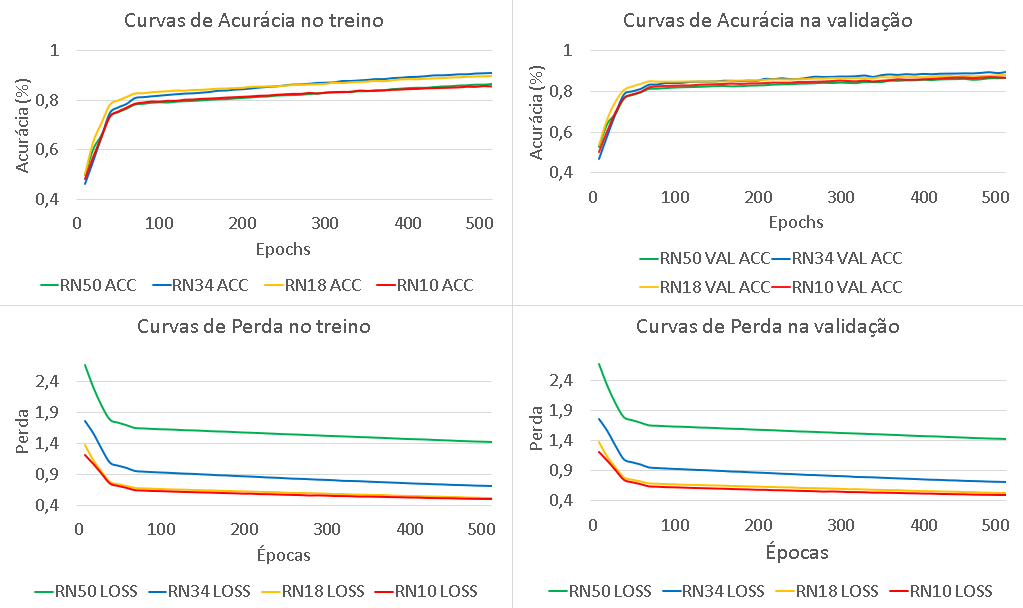
\includegraphics[width=1\linewidth]{figuras/figs_experimentos/resnet_curves}
	\caption{Curvas resultantes do treinamento com os diferentes modelos variantes da arquitetura ResNet. Fonte: o autor.}
	\label{fig:resnetcurves}
\end{figure}

Os resultados obtidos sugerem a existência de um limiar mínimo de complexidade arquitetural necessário para a adequada modelagem do problema. Abaixo desse limiar, a capacidade representacional da rede torna-se insuficiente para capturar relações mais complexas entre as características, limitando o desempenho dos modelos.

Uma vez identificado esse limite estrutural, é importante investigar não apenas a influência da arquitetura, mas também o impacto das configurações de treinamento sobre o desempenho dos modelos, em especial o \textit{batch size} por sua influencia direta sobre a estimativa dos gradientes, o comportamento da convergência. 

\subsection{Avaliação do Impacto do \textit{Batch Size}} 

O tamanho do \textit{batch} desempenha um papel importante na dinâmica de treinamento das redes neurais profundas, influenciando diretamente na capacidade de generalização do modelo. \textit{Batches} menores tendem a introduzir maior variabilidade nas estimativas de gradiente, o que pode atuar como uma forma de regularização implícita, frequentemente resultando em melhor generalização. Por outro lado, \textit{batches} maiores produzem estimativas de gradiente mais estáveis, podendo acelerar a convergência, mas, em alguns casos, levar a uma redução na capacidade de generalização, devido à menor estocasticidade no processo de otimização \cite{keskar2016large}.

Nesse contexto,  foi conduzido um novo conjunto de experimentos focado na análise do impacto do valor de \textit{batch} no desempenho dos modelos mais promissores, definidos no experimento anterior. Para isso, as arquiteturas \textit{ResNet-34} e \textit{ResNet-18} foram novamente treinadas, adotando um aumento no valor do \textit{batch size} de 32 para 64, mantendo-se inalteradas as demais condições experimentais.

Os resultados obtidos com essa nova configuração experimental indicam que valores reduzidos de \textit{batch} se mostraram mais adequados para esse problema, provavelmente devido ao efeito de regularização implícito. Embora o modelo tenha mantido uma dinâmica de treinamento estável, o uso de um \textit{batch} maior não levou a melhorias de desempenho e resultou em uma generalização ligeiramente inferior quando comparado à configuração base, conforme apresentado pela Tabela \ref{tab:comparacao_batchsize_resnet}.

\begin{table}[h]
	\centering
	\caption{Valores resultantes do treinamento conduzido com os modelos \textit{ResNet-18} e \textit{ResNet-34}, considerando um aumento no valor do \textit{Batch Size}.}
	\label{tab:comparacao_batchsize_resnet}
	\setlength{\tabcolsep}{3pt}

		\begin{tabular}{l|c|c|c|c}
			\toprule
			\textbf{Modelo} &
			\makecell{\textbf{Acurácia}\\ \textbf{de Treino}} &
			\makecell{\textbf{Acurácia}\\ \textbf{de Validação}} &
			\makecell{\textbf{Perda}\\ \textbf{(Treino)}} &
			\makecell{\textbf{Perda}\\ \textbf{(Validação)}} \\
			
			\midrule
			
			ResNet-18 (BS = 32)& 0.895 & 0.883 & 0.530 & 0.586 \\
			ResNet-18 (BS = 64) & 0.840 & 0.854 & 0.712 & 0.703 \\
			ResNet-34 (BS = 32)& 0.912 & 0.895 & 0.714 & 0.800 \\
			ResNet-34 (BS = 64) & 0.880 & 0.875 & 0.915 & 0.965 \\
			
			\bottomrule
		\end{tabular}
\end{table}


Um efeito relevante associado à redução do \textit{batch size} é o aumento do número de atualizações de parâmetros realizadas em cada época de treinamento. Como cada atualização passa a utilizar um subconjunto menor de amostras, mais passos de otimização são executados ao longo de cada época, o que pode favorecer uma exploração mais ampla do espaço de parâmetros e facilitar a saída de regiões de mínimo local pouco representativas da função de perda.

Adicionalmente, estudos como o de \cite{masters2018revisiting} indicam que \textit{batches} menores frequentemente apresentam desempenho competitivo ou superior em termos de generalização quando comparados a \textit{batches} maiores, particularmente em cenários nos quais o objetivo principal é maximizar a qualidade preditiva do modelo e não apenas acelerar o processo de treinamento computacional. Com base nesses achados, a configuração com \textit{batch size} igual a 32 foi mantida nos experimentos subsequentes, por apresentar um equilíbrio mais favorável entre estabilidade de convergência e desempenho preditivo. 

% -------------------------------------------------------------------------------
% EXPERIMENTO 6 REFERE-SE AOS SEGUINTES EXPERIMENTOS NA DOCUMENTAÇÃO:
%       •	EXPERIMENTO 14 (RESNET) – TESTE DE 3000 ÉPOCAS COM RESNET18 E BS = 32
% -------------------------------------------------------------------------------

\subsection{Teste Final com a Arquitetura \textit{ResNet}}

Após a identificação das arquiteturas e configurações mais adequadas nos experimentos anteriores, foi conduzido um conjunto final de experimentos com o objetivo de avaliar esses modelos sob um regime de treinamento estendido, totalizando 3000 épocas. O propósito dessa etapa foi investigar se um treinamento prolongado seria capaz de refinar as representações aprendidas, melhorar o desempenho geral dos modelos e, sobretudo, analisar o comportamento de convergência das curvas de aprendizado.

Os resultados, apresentados na Tabela \ref{tab:comparacao_geral} e na Figura \ref{fig:resnetfinal}, indicam que ambas as arquiteturas apresentaram aprendizado consistente e convergência estável ao longo do treinamento. A \textit{ResNet-34} atingiu acurácia máxima de 99,51\% no conjunto de treinamento e 93,74\% no conjunto de validação, enquanto a \textit{ResNet-18} alcançou 99,03\% e 93,42\%, respectivamente. Embora a \textit{ResNet-34} tenha apresentado desempenho ligeiramente superior em termos de acurácia, observa-se que o ganho obtido é marginal.

Em relação à função de perda, a \textit{ResNet-18} apresentou valores mínimos inferiores aos apresentados pela \textit{ResNet-34}, atingindo aproximadamente 0,2424 e 0,5319 para os conjuntos de treinamento e validação, respectivamente. Em contraste, a \textit{ResNet-34} apresentou valores de 0,3768 e 0,7018. Esse resultado sugere que, apesar de sua maior profundidade, a \textit{ResNet-34} não foi capaz de otimizar a função perda de modo mais eficiente nesse cenário específico.

Considerando conjuntamente as métricas de acurácia e perda, bem como a complexidade estrutural dos modelos, a \textit{ResNet-18} destaca-se como a alternativa mais eficiente para a tarefa proposta. Embora a \textit{ResNet-34} apresente ganhos marginais em acurácia, a \textit{ResNet-18} demonstra melhor comportamento de otimização e menor custo computacional, decorrente de sua menor profundidade. Dessa forma, a \textit{ResNet-18} se configura como a escolha mais equilibrada para o problema em estudo, considerando a família de modelos pertencentes à arquitetura \textit{ResNet}.

\begin{figure}[h]
	\centering
	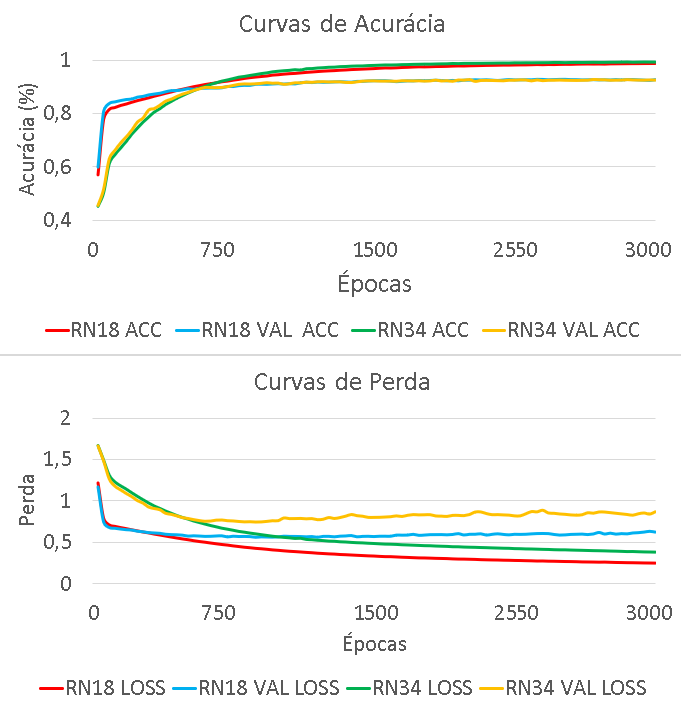
\includegraphics[width=.8\linewidth]{figuras/figs_experimentos/resnet_final}
	\caption{Curvas resultantes do treinamento estendido com as variantes ResNet-18 e ResNet-34. Fonte: o autor.}
	\label{fig:resnetfinal}
\end{figure}


\section{Experimento 3 - Treinamento Conduzido com a Arquitetura \textit{MobileNet}}

Para este experimento, foi conduzido o treinamento da arquitetura \textit{MobileNetV1} com o objetivo de investigar sua eficácia na tarefa de detecção da dor, considerando sua aplicação em cenários com restrições computacionais. Diferentemente de arquiteturas mais profundas e custosas, a \textit{MobileNet} foi projetada para oferecer um bom equilíbrio entre desempenho e eficiência, tornando-se uma alternativa abrangente para implementação em dispositivos com capacidade limitada de processamento.

Embora existam variações mais recentes da arquitetura — como \textit{MobileNetV2} e \textit{MobileNetV3} —, a versão \textit{MobileNetV1} foi selecionada neste estudo por apresentar uma estrutura mais simples e direta, o que facilita a análise isolada do impacto das convoluções separáveis em profundidade. Além disso, por se tratar da formulação original da arquitetura, é possível analisar de forma mais transparente os princípios descritos na literatura \cite{Howard2017}, sem a introdução de mecanismos adicionais, como blocos invertidos ou otimizações específicas de hardware.

Diferentemente das redes convolucionais tradicionais, a \textit{MobileNetV1} utiliza convoluções separáveis em profundidade (\textit{depthwise separable convolutions}), nas quais a operação convolucional padrão é decomposta em duas etapas: uma convolução em profundidade, responsável por aplicar um filtro a cada canal de entrada de forma independente, seguida por uma convolução ponto a ponto, que combina as informações entre os canais. Essa fatoração reduz significativamente o número de parâmetros e o custo computacional do modelo, mantendo sua capacidade de representação.

O modelo adotado segue a arquitetura proposta no trabalho original, no entanto, algumas adaptações foram introduzidas com o objetivo de adequá-lo ao cenário experimental deste estudo, conforme apresentado na Tabela \ref{tab:mobilenet_str}. Dentre as alterações, o multiplicador de largura foi ajustado para $\alpha = 0.75$ a fim de reduzir o número de canais em cada camada e, consequentemente, a complexidade geral do modelo.

Adicionalmente, foi inserida uma camada de \textit{Dropout} com taxa de $0.3$ após a etapa de \textit{global average pooling}, com o intuito de melhorar a capacidade de generalização. Também foi aplicada regularização L2 ($\lambda = 5 \times 10^{-5}$) nas camadas convolucionais e na camada totalmente conectada, buscando reduzir o risco de \textit{overfitting}, especialmente considerando o tamanho reduzido do conjunto de dados utilizado.

Por fim, as imagens de entrada foram redimensionadas para $160 \times 160 \times 3$, buscando um equilíbrio entre preservação da informação espacial e o custo computacional para a \textit{MobileNet}. Demais configurações adotadas para o treinamento encontram-se descritas na Tabela \ref{tab:unified_training_config}. 

\begin{table}[h]
	\centering
	\caption{Resultados médios das últimas 15 épocas no treinamento conduzido com a modelo \textit{MobileNet-V1}}
	\label{tab:results_mobilenet}
	\setlength{\tabcolsep}{3pt}
	
	\begin{tabular}{l|c|c|c|c}
		\toprule
		\textbf{Modelo} &
		\makecell{\textbf{Acurácia}\\ \textbf{de Treino}} &
		\makecell{\textbf{Acurácia}\\ \textbf{de Validação}} &
		\makecell{\textbf{Perda}\\ \textbf{(Treino)}} &
		\makecell{\textbf{Perda}\\ \textbf{(Validação)}} \\
		\midrule
		
		MobileNet - V1 & 0.9920 & 0.8605 & 0.1029 & 1.0241 \\

		\bottomrule
	\end{tabular}
\end{table}

Os resultados apresentados pela Tabela \ref{tab:results_mobilenet}, indicam que o modelo foi capaz de atingir elevada acurácia no conjunto de treinamento ao longo do processo de otimização. A acurácia média nas últimas 15 épocas foi de aproximadamente 99.20\%, com valor correspondente na perda de 0.1029. Entretanto, observa-se uma diferença mais expressiva entre os valores obtidos nos conjuntos de treinamento e validação. A acurácia média de validação atingiu 86.05\%, enquanto a função de perda estabilizou em 1.0241.

Essa discrepância sugere a presença de um leve grau de \textit{overfitting}, no qual o modelo se torna altamente especializado nos dados de treinamento, mas apresenta limitações na capacidade de generalização para dados não vistos. Esse comportamento pode ser atribuído à menor capacidade representacional da arquitetura quando comparada a modelos mais profundos, bem como ao tamanho reduzido do conjunto de dados utilizado.

De modo geral, os resultados indicam que o modelo testado se mostra como uma alternativa viável para cenários nos quais a eficiência computacional é um fator crítico, no entanto, seu desempenho foi inferior ao observado para a arquitetura \textit{ResNet-18} — previamente avaliada neste estudo. Dessa forma, embora a \textit{MobileNetV1} apresente vantagens em termos de custo computacional, sua utilização como modelo principal para a tarefa proposta mostra-se menos vantajosa.

Cabe destacar que foram conduzidos experimentos adicionais com pequenas variações nos hiperparâmetros, a fim de mitigar o \textit{overfitting} observado. No entanto, tais ajustes não resultaram em melhorias significativas. 

\section{Experimento 4 - Treinamento Conduzido com a Arquitetura \textit{DenseNet}}

Neste experimento, foi avaliada uma arquitetura personalizada baseada na \textit{DenseNet}, com o objetivo de investigar o impacto da conectividade densa e do reaproveitamento extensivo de características na tarefa de classificação considerada neste estudo. Diferentemente das redes convolucionais tradicionais, a \textit{DenseNet} estabelece conexões diretas entre todas as camadas dentro de um mesmo bloco denso, permitindo que cada camada receba como entrada os mapas de características de todas as camadas anteriores \cite{Huang2017}.

Esse mecanismo favorece a propagação de informação e gradientes ao longo da rede, além de promover um uso mais eficiente das representações aprendidas. Tais propriedades são relevantes em cenários com conjuntos reduzido de dados e em tarefas que envolvem padrões visuais sutis, como aqueles definidos pela \acs{MGS}, nos quais a preservação de informações em múltiplos níveis de abstração pode contribuir para um melhor desempenho do modelo.

Inicialmente, foram conduzidos testes preliminares utilizando a arquitetura padrão \textit{DenseNet-121}. No entanto, foi proposta uma versão personalizada com o objetivo de reduzir a complexidade computacional do modelo, alinhado com a estratégia adotada no experimento com a \textit{MobileNet}, que buscou avaliar arquiteturas mais eficientes para viabilizar sua implementação em ambientes com restrições computacionais. Uma comparação estrutural das camadas densas entre o modelo base e a configuração customizada proposta é apresentada na Tabela \ref{tab:densenet_comparison}.

\begin{table}[h]
	\centering
	\caption{Comparativo entre o modelo \textit{DenseNet-121} e o modelo customizado mais raso da \textit{DenseNet}.}
	\label{tab:densenet_comparison}
	\renewcommand{\arraystretch}{1.8}
	
	\resizebox{\textwidth}{!}{
		\begin{tabular}{lcc}
			\toprule
			\textbf{Camada} & \textbf{Modelo Customizado} & \textbf{DenseNet-121 (Padrão)} \\
			\midrule
			
			Conv1 
			& $3 \times 3$, 48 filters 
			& $7 \times 7$, 64 filters, stride 2 + MaxPool \\
			
			Dense Block 1 
			& 6 layers, $k=24$ 
			& 6 layers, $k=32$ \\        
			
			Transition 1 
			& $1 \times 1$ conv + AvgPool ($\theta = 0.5$) 
			& $1 \times 1$ conv + AvgPool ($\theta = 0.5$) \\ 
			
			Dense Block 2 
			& 8 layers, $k=24$ 
			& 12 layers, $k=32$ \\        
			
			Transition 2 
			& $1 \times 1$ conv + AvgPool ($\theta = 0.5$) 
			& $1 \times 1$ conv + AvgPool ($\theta = 0.5$) \\
			
			Dense Block 3 
			& 12 layers, $k=24$ 
			& 24 layers, $k=32$ \\
			
			Transition 3 
			& $1 \times 1$ conv + AvgPool ($\theta = 0.5$) 
			& $1 \times 1$ conv + AvgPool ($\theta = 0.5$) \\
			
			Dense Block 4 
			& 8 layers, $k=24$ 
			& 16 layers, $k=32$ \\
			
			\midrule
			
			Batch Normalization + \acs{ReLU} 
			&  \multicolumn{2}{c}{Camada final de normalização seguida por ativação \acs{ReLU} } \\  
			
			AvgPool 
			&  \multicolumn{2}{c}{Camada de extração global das características - Global Average Pooling} \\
			
			Dropout 
			& 0.3 
			& Não utilizado na estrutura padrão \\
			
			Fully Conected 
			& \multicolumn{2}{c}{Camada totalmente conectada} \\
		
			\bottomrule
		\end{tabular}
	}
\end{table}

Os resultados obtidos com ambas as configurações mostraram-se semelhantes, com diferenças marginais tanto em termos de acurácia quanto de perda, conforme descrito na tabela \ref{tab:densenet_variants_results}. Esse comportamento sugere que a capacidade representacional completa da \textit{DenseNet-121} não é estritamente necessária para a tarefa considerada. Dessa forma, optou-se pela utilização da arquitetura personalizada, que apresenta menor custo computacional, mantendo desempenho competitivo.

\begin{table}[h]
	\centering
	\caption{Resultados obtidos pelo treinamento conduzido com ambos os modelos baseados na arquitetura \textit{\textit{DenseNet}} (\textit{DenseNet-121} e \textit{DenseNet} Customizado)}
	\label{tab:densenet_variants_results}
	\setlength{\tabcolsep}{3pt}
	
	\begin{tabular}{l|c|c|c|c}
		\toprule
		\textbf{Modelo} &
		\makecell{\textbf{Acurácia}\\ \textbf{de Treino}} &
		\makecell{\textbf{Acurácia}\\ \textbf{de Validação}} &
		\makecell{\textbf{Perda}\\ \textbf{(Treino)}} &
		\makecell{\textbf{Perda}\\ \textbf{(Validação)}} \\
		\midrule
		
		DenseNet-121 & 0.9985 & 0.9171 & 0.0069 & 0.3707 \\
		DenseNet Customizada & 0.9918 & 0.9182 & 0.0286 & 0.3051 \\

		\bottomrule
	\end{tabular}
\end{table}

Conforme observado no experimento anterior, o processo de treinamento foi interrompido de forma antecipada em função da estabilização das métricas de validação, indicando que o modelo atingiu um regime de convergência no qual variações adicionais nos indicadores de desempenho se tornaram marginais. 

Entretanto, considerando a velocidade elevada de convergência apresentada pela arquitetura \textit{DenseNet}, foi conduzido um experimento adicional utilizando a mesma configuração de treinamento, porém forçando a continuidade do processo até o total de 500 épocas. O objetivo dessa análise consistiu em verificar se a estabilização precoce das métricas correspondia, de fato, a um regime estável de convergência ou se treinamentos mais prolongados poderiam resultar em ganhos adicionais de desempenho. Os resultados correspondentes encontram-se ilustrados na Figura \ref{fig:denseNet500}.

\begin{figure}[h]
	\centering
	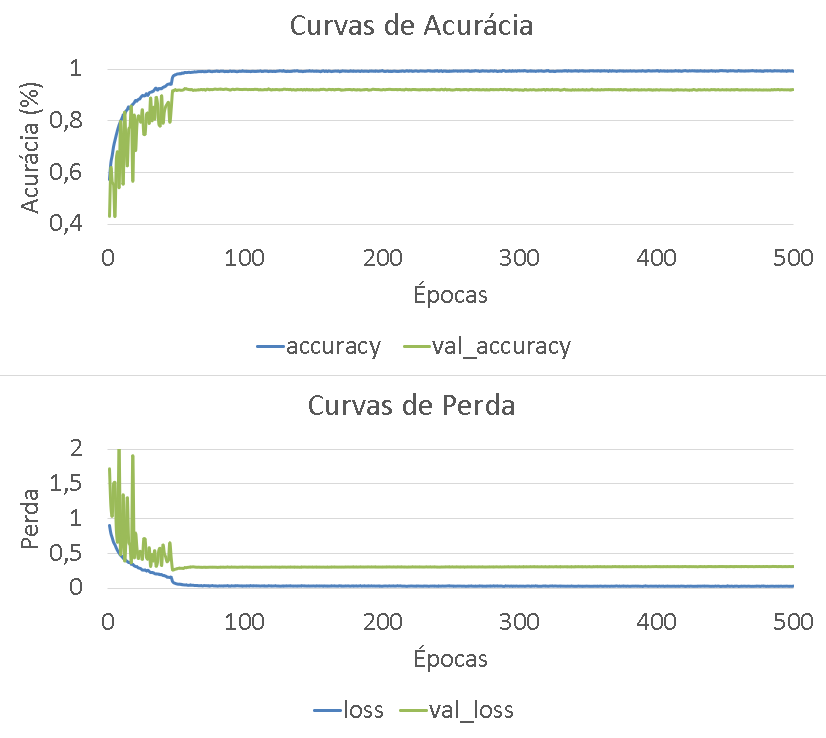
\includegraphics[width=.7\linewidth]{figuras/figs_experimentos/densenet_500eps}
	\caption{Curvas resultantes do treinamento conduzido com a DenseNet por todas as 500 épocas. Fonte: o autor.}
	\label{fig:denseNet500}
\end{figure}

Testes adicionais conduzidos com valores mais elevados de \textit{batch size} resultaram em erros de insuficiência de memória logo nas etapas iniciais do treinamento, inviabilizando a continuidade da execução sob as limitações de hardware disponíveis. As demais configurações de treinamento adotadas encontram-se detalhadas na Tabela \ref{tab:unified_training_config}.

Os resultados obtidos com o modelo customizado, calculados a partir da média das últimas 15 épocas (Tabela \ref{tab:densenet_variants_results}), apresentam um desempenho elevado tanto no conjunto de treinamento quanto no de validação. Diferentemente do que foi observado no experimento conduzido com a \textit{MobileNet}, os valores resultantes nos conjuntos de treino e validação apresentam uma proximidade maior, indicando um processo de aprendizado mais equilibrado e uma capacidade de generalização superior.



Quando comparada às arquiteturas avaliadas anteriormente, a \textit{DenseNet} mantém níveis de acurácia de treinamento semelhantes aos obtidos com a \textit{ResNet}, ao mesmo tempo em que apresenta desempenho superior no conjunto de validação em relação à \textit{MobileNet}, além de um menor desvio entre treinamento e validação. Esses resultados indicam que o mecanismo de reaproveitamento de características contribui fortemente para a captura de padrões visuais sutis associados à dor.

Adicionalmente, considerando os baixos valores de perda observados tanto no treinamento quanto na validação, os resultados sugerem que a arquitetura \textit{DenseNet} modificada apresenta um ajuste mais adequado ao problema proposto. Nesse contexto, o modelo pode ser considerado uma alternativa competitiva e, em alguns aspectos, superior à \textit{ResNet-18}, especialmente no que se refere à capacidade de generalização. 

\section{Experimento 5 - Utilização da Arquitetura \textit{Vision Transformer}}

Neste experimento, foi investigado o comportamento da arquitetura \acs{VIT}, baseada em um paradigma distinto daquele adotado pelas redes convolucionais tradicionais, especialmente no que se refere ao processamento das informações espaciais presentes na imagem. Enquanto as \acsp{CNN} utilizam operações convolucionais para extração hierárquica de padrões locais, os modelos \acs{VIT} tratam a imagem como uma sequência de \textit{patches}, processados por mecanismos de autoatenção (\textit{self-attention}) originalmente propostos para tarefas de processamento de linguagem natural.

A utilização da arquitetura \acs{VIT} é relevante no contexto deste trabalho devido à natureza da \acs{MGS}, cuja avaliação depende da análise conjunta de múltiplas regiões faciais para identificação de expressões sutis associadas à dor. Diferentemente das \acsp{CNN}, os modelos baseados em \textit{Transformers} apresentam menor viés indutivo relacionado à localidade espacial e à invariância translacional, aprendendo essas relações diretamente a partir dos dados durante o treinamento.

Entretanto, essa característica também torna os modelos \acs{VIT} mais dependentes de grandes volumes de dados para treinamento eficiente, especialmente em arquiteturas profundas e altamente parametrizadas. Considerando o tamanho moderado da base de dados utilizada neste estudo, o treinamento foi conduzido utilizando técnicas de \textit{Transfer Learning} e congelamento parcial de camadas (\textit{layer freezing}), empregando pesos pré-treinados na base \textit{ImageNet-21k} para a arquitetura \textit{\acs{VIT}-B/16}, disponibilizados pelo repositório oficial da \textit{Google Research}.

A estratégia de congelamento parcial consistiu em impedir a atualização dos pesos das camadas intermediárias da rede durante o treinamento, permitindo o refinamento apenas das camadas finais responsáveis pela especialização da tarefa. Essa abordagem possibilitou preservar representações visuais gerais previamente aprendidas em bases de larga escala, reduzindo a necessidade de treinamento completo da arquitetura a partir de inicialização aleatória.

Inicialmente, o treinamento foi conduzido durante 500 épocas. Posteriormente, com o objetivo de investigar o comportamento de convergência da arquitetura em treinamentos prolongados, o experimento foi estendido para 800 épocas utilizando a mesma configuração experimental. Os resultados médios obtidos a cada intervalo de 100 épocas são apresentados na Tabela \ref{tab:vit_mean_results_800}.

\begin{table}[h]
	\centering
	\caption{Média dos valores de acurácia e perda obtidos a cada intervalo de 100 épocas durante o treinamento da arquitetura \acs{VIT}.}
	\label{tab:vit_mean_results_800}
	\begin{tabular}{l|c|c|c|c}
		
		\toprule
		\makecell{\textbf{Faixa} \\ \textbf{de épocas}}&
		\makecell{\textbf{Acurácia}\\ \textbf{de treino}} &
		\makecell{\textbf{Acurácia}\\ \textbf{de validação}} &
		\makecell{\textbf{Perda}\\ \textbf{(treino)}} &
		\makecell{\textbf{Perda}\\ \textbf{(validação)}} \\
		\midrule
		
		001-100 & 0.9038 & 0.7519 & 0.4536 & 0.6839 \\
		101-200 & 0.9808 & 0.7982 & 0.3265 & 0.6318 \\
		201-300 & 0.9904 & 0.8212 & 0.3092 & 0.5787 \\
		301-400 & 0.9938 & 0.8255 & 0.3028 & 0.5771 \\
		401-500 & 0.9956 & 0.8239 & 0.2996 & 0.5905 \\
		501-600 & 0.9967 & 0.8204 & 0.2975 & 0.6054 \\
		601-700 & 0.9975 & 0.8262 & 0.2959 & 0.5957 \\
		701-800 & 0.9981 & 0.8354 & 0.2947 & 0.5697 \\
		
		\bottomrule
	\end{tabular}
\end{table}

\begin{comment}
	\begin{table}[h]
		\centering
		\caption{Média dos valores resultantes a cada 100 épocas do treinamento conduzido com a arquitetura \acs{VIT}.}
		\label{tab:vit_mean_results}
		\begin{tabular}{l|c|c|c|c}
			
			\toprule
			\makecell{\textbf{Faixa} \\ \textbf{de épocas}}&
			\makecell{\textbf{Acurácia}\\ \textbf{de Treino}} &
			\makecell{\textbf{Acurácia}\\ \textbf{de Validação}} &
			\makecell{\textbf{Perda}\\ \textbf{(Treino)}} &
			\makecell{\textbf{Perda}\\ \textbf{(Validação)}} \\
			\midrule
			
			001-100 & 0.9046 & 0.7598 & 0.4523 & 0.6577 \\
			101-200  & 0.9808 & 0.79985 & 0.3265 & 0.6296 \\
			201-300 & 0.9909 & 0.8141 & 0.30834 & 0.6065 \\
			301-400 & 0.9946 & 0.8219 & 0.3015 & 0.5908 \\
			401-500 & 0.9966 & 0.8252 & 0.2976 & 0.5916 \\
			
			\bottomrule
		\end{tabular}
	\end{table}
\end{comment}

Os resultados apresentados na Tabela \ref{tab:vit_mean_results_800} correspondem às médias dos valores de acurácia e perda obtidos nos conjuntos de treinamento e validação, calculadas a cada intervalo de 100 épocas. Essa estratégia permite observar de forma mais clara a evolução do desempenho da arquitetura ao longo do treinamento, minimizando oscilações pontuais e evidenciando tendências gerais de convergência.

Observa-se que a arquitetura apresenta rápida convergência nas primeiras 200 épocas, seguida por um regime de estabilização caracterizado por ganhos marginais nas métricas avaliadas. Esse comportamento pode ser parcialmente explicado pela utilização combinada de \textit{Transfer Learning} e congelamento parcial das camadas da rede.

Como a maior parte da arquitetura já havia sido previamente treinada na base \textit{ImageNet-21k}, o modelo iniciou o processo de refinamento com representações visuais previamente estruturadas, reduzindo significativamente a necessidade de aprender padrões básicos a partir de uma inicialização aleatória. Além disso, o congelamento das camadas intermediárias favoreceu a maior estabilidade durante o treinamento e adaptação mais rápida ao domínio específico da tarefa proposta.

Os resultados obtidos indicam que a arquitetura foi capaz de aprender padrões relevantes para a tarefa de classificação, evidenciado pela redução consistente da função de perda e pelo aumento progressivo da acurácia ao longo do treinamento. Entretanto, observa-se um comportamento característico de \textit{overfitting}, uma vez que os elevados valores de acurácia obtidos no conjunto de treinamento não são acompanhados proporcionalmente pelo conjunto de validação, embora este também apresente desempenho satisfatório.

Além disso, o prolongamento do treinamento até 800 épocas produziu ganhos relativamente modestos no desempenho de validação quando comparado às primeiras etapas do treinamento, sugerindo que a arquitetura atinge rapidamente um regime próximo da estabilização para o conjunto de dados utilizado neste estudo. Para melhor visualização do comportamento de convergência da arquitetura, a Figura \ref{fig:vitcurves} apresenta as curvas de acurácia e perda obtidas ao longo do treinamento.


\begin{figure}[h]
	\centering
	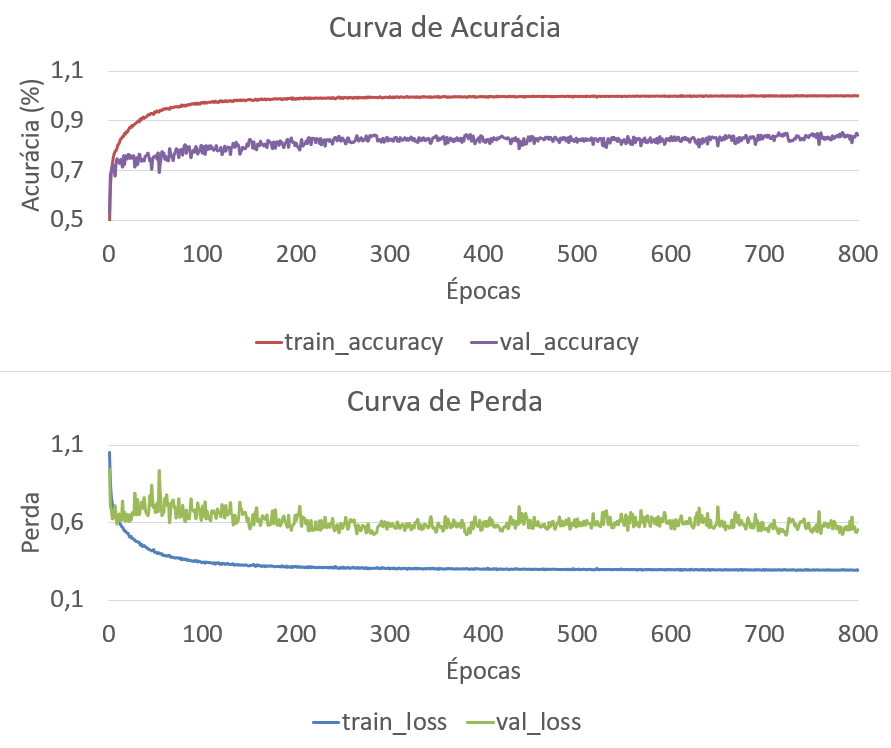
\includegraphics[width=0.8\linewidth]{figuras/figs_experimentos/vit_800eps.png}
	\caption{Curvas de acurácia e perda para o treinamento conduzido com a arquitetura \acs{VIT}. Fonte: o autor.}
	\label{fig:vitcurves}
\end{figure}

\subsection{Treinamento Conduzido com uma Redução no Conjunto de Treino}

O comportamento de \textit{overfitting} observado no experimento anterior sugere que o desempenho da arquitetura \acs{VIT} pode estar diretamente associado à quantidade de dados disponíveis durante o treinamento. Considerando a elevada capacidade representacional dos modelos baseados em \textit{Transformers}, mesmo sob estratégias de \textit{Transfer Learning} e congelamento parcial de camadas, foi conduzido um experimento adicional com redução controlada da base de treinamento, com o objetivo de investigar a sensibilidade da arquitetura à disponibilidade de amostras.

A hipótese considerada neste experimento é que a diminuição da quantidade de dados disponíveis para treinamento reduz a diversidade de padrões visuais apresentados ao modelo, comprometendo sua capacidade de adaptação ao conjunto de validação. Consequentemente, espera-se observar redução dos valores de acurácia e aumento da função de perda durante o processo de avaliação.

Para isso, foi conduzido um novo treinamento utilizando a mesma configuração experimental adotada anteriormente para a arquitetura \acs{VIT}, diferenciando-se apenas pela redução do conjunto de dados destinado ao treinamento. O número de imagens pertencentes a cada classe da base de dados (\textit{Indolor}, \textit{Pouca Dor} e \textit{Muita Dor}) foi reduzido pela metade por meio de remoção aleatória e balanceada das amostras. Essa estratégia permitiu preservar a proporcionalidade entre as classes, evitando a introdução de desequilíbrios que pudessem comprometer a interpretação dos resultados.

Os resultados apresentados na Tabela \ref{tab:vit_reduced_data_mean_results} correspondem às médias dos valores de acurácia e perda obtidos nos conjuntos de treinamento e validação, calculadas a cada intervalo de 100 épocas. Essa abordagem permite observar a evolução do desempenho da arquitetura ao longo do treinamento, minimizando oscilações pontuais nas métricas avaliadas.

\begin{table}[h]
	\centering
	\caption{Média dos valores resultantes a cada 100 épocas do treinamento conduzido com a arquitetura \acs{VIT}, considerando a redução aplicada nas amostras para o conjunto de treino.}
	\label{tab:vit_reduced_data_mean_results}
	\begin{tabular}{l|c|c|c|c}
		
		\toprule
		\makecell{\textbf{Faixa} \\ \textbf{de épocas}}&
		\makecell{\textbf{Acurácia}\\ \textbf{de Treino}} &
		\makecell{\textbf{Acurácia}\\ \textbf{de Validação}} &
		\makecell{\textbf{Perda}\\ \textbf{(Treino)}} &
		\makecell{\textbf{Perda}\\ \textbf{(Validação)}} \\
		\midrule
		
		001-100 & 0.9427 & 0.7458 & 0.3912 & 0.7235 \\
		101-200 & 0.9909 & 0.7591 & 0.3084 & 0.7641 \\
		201-300 & 0.9953 & 0.7639 & 0.3005 & 0.7839 \\
		301-400 & 0.9970 & 0.7671 & 0.2968 & 0.7891 \\
		401-500 & 0.9981 & 0.7761 & 0.2947 & 0.7691 \\
		
		\bottomrule
	\end{tabular}
\end{table}

Os resultados obtidos permanecem consistentes com o comportamento observado no experimento anterior, evidenciando rápida convergência da arquitetura nas primeiras 200 épocas de treinamento, seguida por um regime de estabilização das métricas avaliadas. Entretanto, o comportamento de \textit{overfitting} torna-se significativamente mais pronunciado nesse novo cenário experimental.

Observa-se que, embora a acurácia do conjunto de treinamento permaneça elevada ao longo das épocas, o desempenho obtido no conjunto de validação apresenta redução consistente quando comparado ao experimento conduzido com a base completa. Paralelamente, os valores da função de perda tornam-se progressivamente maiores no conjunto de validação, indicando maior dificuldade da arquitetura em adaptar-se a dados não observados durante o treinamento.

Esses resultados sugerem que, mesmo utilizando estratégias de \textit{Transfer Learning}, as arquiteturas baseadas em \textit{Transformers} permanecem altamente dependentes da disponibilidade de dados para construção de representações robustas. Tal comportamento está alinhado com o observado na literatura, na qual modelos \acs{VIT} frequentemente apresentam maior sensibilidade ao tamanho da base de treinamento quando comparados às arquiteturas convolucionais tradicionais. Para melhor visualização do comportamento de convergência e das diferenças entre os conjuntos de treinamento e validação, a Figura \ref{fig:vitcurves_reduced} apresenta graficamente a evolução das métricas ao longo do treinamento.

\begin{figure}[h]
	\centering
	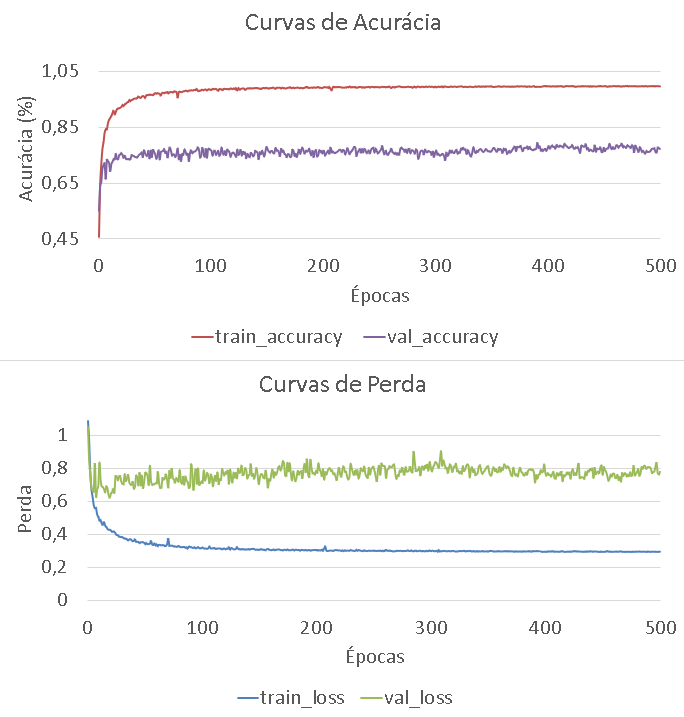
\includegraphics[width=.75\linewidth]{figuras/figs_experimentos/vit_reduced_curves}
	\caption{Curvas de acurácia e perda para o treinamento conduzido com a arquitetura \acs{VIT}, considerando uma redução na base de dados. Fonte: o autor.}
	\label{fig:vitcurves_reduced}
\end{figure}

\subsection{Treinamento Conduzido com uma Alteração na Divisão da Base de Dados}

Além do experimento envolvendo redução controlada da base de treinamento, foi conduzida uma análise adicional com modificação da estratégia de divisão dos subconjuntos de treinamento e validação. O objetivo desse experimento consistiu em investigar o impacto da distribuição das amostras sobre o comportamento das métricas de validação e sobre a estabilidade do processo de avaliação da arquitetura.

Na configuração originalmente adotada com uma divisão de 80/20 por cento, o modelo dispõe de maior quantidade de amostras para aprendizado, favorecendo a construção de representações visuais mais robustas durante o treinamento. Entretanto, em cenários envolvendo bases de dados moderadas — como o presente estudo — conjuntos de validação mais reduzidos podem apresentar maior sensibilidade a flutuações estatísticas, dificultando uma representação mais consistente da variabilidade real dos dados. Dessa forma, optou-se por conduzir um novo experimento utilizando uma divisão de 70/30 entre os conjuntos de treinamento e validação, respectivamente.

Nessa nova configuração, parte das amostras originalmente destinadas ao treinamento passam a compor o conjunto de validação, ampliando a quantidade de exemplos utilizados durante a avaliação do modelo. Embora essa estratégia reduza parcialmente a quantidade de dados disponíveis para aprendizado, ela possibilita uma análise potencialmente mais representativa do comportamento da arquitetura durante a validação.

O treinamento foi conduzido utilizando a mesma configuração experimental adotada anteriormente para a arquitetura \acs{VIT}, diferenciando-se apenas pela nova proporção utilizada na divisão da base de dados. Assim como nos experimentos anteriores, o treinamento foi executado durante 800 épocas, com o objetivo de assegurar estabilização adequada das métricas avaliadas. Os valores médios obtidos a cada intervalo de 100 épocas são apresentados na Tabela \ref{tab:vit_7030_results}.

\begin{table}[h]
	\centering
	\caption{Média dos valores resultantes a cada 100 épocas do treinamento conduzido com a arquitetura \acs{VIT}, considerando a divisão da base de dados 70/30\% para os conjuntos de treino e validação, respectivamente.}
	\label{tab:vit_7030_results}
	\begin{tabular}{l|c|c|c|c}
		
		\toprule
		\makecell{\textbf{Faixa} \\ \textbf{de épocas}}&
		\makecell{\textbf{Acurácia}\\ \textbf{de Treino}} &
		\makecell{\textbf{Acurácia}\\ \textbf{de Validação}} &
		\makecell{\textbf{Perda}\\ \textbf{(Treino)}} &
		\makecell{\textbf{Perda}\\ \textbf{(Validação)}} \\
		\midrule
		
		001-100 & 0.9363 & 0.8070 & 0.4003 & 0.5478 \\
		101-200 & 0.9873 & 0.8447 & 0.3147 & 0.5007 \\
		201-300 & 0.9931 & 0.8553 & 0.3043 & 0.4797 \\
		301-400 & 0.9954 & 0.8617 & 0.2998 & 0.4675 \\
		401-500 & 0.9967 & 0.8645 & 0.2974 & 0.4647 \\
		501-600 & 0.9976 & 0.8637 & 0.2958 & 0.4726 \\
		601-700 & 0.9981 & 0.8685 & 0.2947 & 0.4595 \\
		701-800 & 0.9986 & 0.8715 & 0.2938 & 0.4558 \\
		
		\bottomrule
	\end{tabular}
\end{table}

Os resultados obtidos indicam comportamento semelhante ao observado nos experimentos anteriores, caracterizado por rápida convergência da arquitetura nas primeiras épocas de treinamento, seguida por estabilização gradual das métricas de desempenho. Entretanto, observa-se melhora consistente dos resultados obtidos no conjunto de validação quando comparados à configuração original utilizando divisão 80/20. 

Esse comportamento sugere que o aumento da quantidade de amostras destinadas ao subconjunto de validação contribuiu para uma avaliação mais estável e representativa do desempenho da arquitetura. Ainda assim, deve-se considerar que a redução do conjunto de treinamento também implica menor quantidade de dados disponíveis para aprendizado, configurando um compromisso entre capacidade de treinamento e robustez estatística da validação.

Além disso, embora os resultados indiquem redução relativa do comportamento de \textit{overfitting} quando comparados aos experimentos anteriores, ainda permanece uma diferença significativa entre os desempenhos observados nos conjuntos de treinamento e validação, indicando que a limitação relacionada à disponibilidade de dados continua impactando o comportamento da arquitetura. A Figura \ref{fig:vitcurves_70/30} apresenta as curvas de acurácia e perda obtidas durante o treinamento utilizando a divisão 70/30 da base de dados.

\begin{figure}[h]
	\centering
	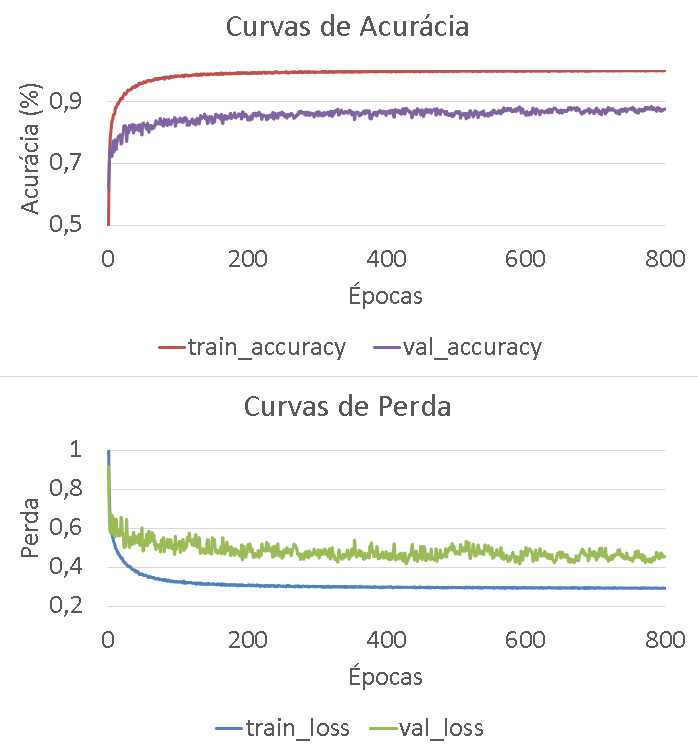
\includegraphics[width=.7\linewidth]{figuras/figs_experimentos/vit_new_data_div}
	\caption{Curvas de acurácia e perda para o treinamento conduzido com a arquitetura \acs{VIT}, considerando a divisão de 70/30 na base de dados. Fonte: o autor.}
	\label{fig:vitcurves_70/30}
\end{figure}

\subsection{Considerações Finais}

Os resultados experimentais obtidos ao longo deste estudo evidenciam aspectos relevantes acerca da aplicabilidade de classificadores neurais para a avaliação automatizada da dor com base na \acs{MGS}. A Tabela \ref{tab:comparacao_geral} apresenta uma visão consolidada dos principais resultados obtidos nos experimentos conduzidos.

Entre os modelos avaliados, as arquiteturas convolucionais fundamentadas no reaproveitamento e na propagação eficiente de características apresentaram desempenho superior. Em especial, os modelos \textit{ResNet}-18 e \textit{DenseNet (Customizado)} obtiveram os melhores resultados gerais, combinando elevados valores de acurácia e expressiva redução na perda. Adicionalmente, observa-se uma forte proximidade nos desempenhos resultantes para os conjuntos de treinamento e validação, o que implica em uma boa capacidade de generalização.

Tais resultados sugerem que mecanismos intensivos de reutilização de características, aliados a um equilíbrio adequado entre profundidade arquitetural e capacidade de representação, constituíram alguns dos principais fatores responsáveis pela eficiência observada na tarefa de classificação proposta. Considerando que as expressões faciais associadas à dor foram caracterizadas por padrões visuais bem definidos, a preservação e reutilização de representações intermediárias ao longo da rede parecem desempenhar um papel importante na melhoria da capacidade de generalização dos modelos.

Além disso, os resultados obtidos com a arquitetura \textit{DenseNet} customizada representam uma contribuição relevante deste trabalho. Embora apresente menor profundidade e complexidade computacional quando comparada ao modelo de referência \textit{DenseNet}-121, a arquitetura proposta foi capaz de manter desempenho competitivo. Dessa forma, a configuração desenvolvida amplia a viabilidade da utilização de estratégias baseadas em conectividade densa, inclusive em cenários caracterizados por restrições computacionais mais severas.

Em contrapartida, embora a arquitetura \textit{MobileNetV1} tenha apresentado comportamento de \textit{overffiting} mais acentuado, com métricas de validação significativamente inferiores às observadas durante o treinamento, seu projeto orientado à eficiência computacional ainda a torna uma alternativa relevante para aplicações em sistemas embarcados e soluções de monitoramento em tempo real. Em cenários nos quais os benefícios proporcionados pela reutilização intensiva de características não se mostrem expressivos, arquiteturas leves como a \textit{MobileNetV1} podem representar um compromisso interessante entre desempenho preditivo e custo computacional.

Outra observação importante refere-se à influência dos parâmetros de configuração do treinamento, especialmente à escolha no tamanho do (\textit{batch size}). Os experimentos conduzidos com as arquiteturas da família \textit{ResNet} indicaram que lotes menores favoreceram o desempenho no conjunto de validação e contribuíram para a redução do \textit{overfitting}, particularmente em bases de dados com tamanho moderado e em tarefas envolvendo padrões faciais sutis.

Esse comportamento pode estar associado ao efeito de regularização implícita decorrente da maior variabilidade presente na estimativa dos gradientes durante o processo de otimização. Tal observação está em conformidade com resultados previamente reportados na literatura de aprendizado profundo, que apontam o uso de lotes menores como um fator potencialmente benéfico para a capacidade de generalização dos modelos.

\begin{table*}[h]
	\centering
	\caption{Resultados agregados dos experimentos conduzidos com as diferentes arquiteturas de redes neurais.}
	\label{tab:comparacao_geral}
	\renewcommand{\arraystretch}{1.3}
	
	\begin{tabular}{l|c|c|c|c|c|c}
		\toprule
		
		\makecell{\textbf{Modelo}}&
		\makecell{\textbf{Épocas}}&
		\makecell{\textbf{Batch}\\ \textbf{Size}}&
		\makecell{\textbf{Acurácia}\\ \textbf{(Treino)}} &
		\makecell{\textbf{Acurácia}\\ \textbf{(Val.)}} &
		\makecell{\textbf{Perda}\\ \textbf{(Treino)}} &
		\makecell{\textbf{Perda}\\ \textbf{(Val.)}} \\
		\midrule

		ResNet-50 & 500 & 32 & 0.864 & 0.869 & 1.433 & 1.451 \\
		ResNet-34 & 3000 & 32 & 0.995 & 0.937 & 0.376 & 0.701 \\
		ResNet-34 & 500 & 64 & 0.880 & 0.875 & 0.915 & 0.965 \\
		ResNet-18 & 3000 & 32 & 0.990 & 0.934 & 0.242 & 0.531 \\
		ResNet-18 & 500 & 64 & 0.840 & 0.854 & 0.712 & 0.703 \\
		ResNet-10 & 500 & 32 & 0.856 & 0.869 & 0.501 & 0.480 \\
		MobileNet-V1 & 500 & 32 & 0.992 & 0.860 & 0.102 & 1.024 \\
		DenseNet-121 & 500 & 16 & 0.998 & 0.917 & 0.006 & 0.370 \\
		DenseNet C. & 500 & 16 & 0.991 & 0.918 & 0.028 & 0.305 \\
		\acs{VIT} & 800 & 16 & 0.998 & 0.835 & 0.294 & 0.569 \\
		\acs{VIT} (70/30) & 800 & 16 & 0.998 & 0.871 & 0.293 & 0.455 \\
		
		\bottomrule
		
	\end{tabular}
\end{table*}

Considerando os experimentos conduzidos com o modelo \acs{VIT}, os resultados evidenciaram a presença consistente de \textit{overfitting}, caracterizada pela diferença relativamente elevada entre os desempenhos observados nos conjuntos de treinamento e validação. Esse comportamento foi observado mesmo com a utilização de \textit{Transfer Learning} a partir de pesos previamente treinados na base \textit{ImageNet-21k}. Adicionalmente, a redução controlada das amostras disponíveis para treinamento reforçou essa observação, resultando em degradação significativa das métricas de validação.

Diferentemente das redes convolucionais tradicionais, que incorporam explicitamente propriedades estruturais importantes para o processamento de imagens — como localidade espacial, compartilhamento de pesos e invariância translacional — os modelos \acs{VIT} não assumem previamente essas relações, como consequência, arquiteturas baseadas em \textit{Transformers} tendem a demandar conjuntos de dados significativamente maiores para alcançar desempenho mais robusto em tarefas de classificação visual.

Esse comportamento sugere que o desempenho da arquitetura está fortemente associado à diversidade e à quantidade de dados disponíveis, característica amplamente reportada na literatura para modelos baseados em \textit{Transformers}. Ainda assim, os resultados obtidos podem ser considerados satisfatórios, especialmente quando se considera o tamanho relativamente limitado da base de dados utilizada e a natureza especializada da tarefa de classificação proposta.

Nesse contexto, o principal fator limitante para a melhoria do desempenho da arquitetura não está necessariamente relacionado à sua capacidade representacional, nem exclusivamente à configuração dos hiperparâmetros empregados, mas sobretudo à disponibilidade de dados para treinamento. Embora estratégias adicionais de otimização possam contribuir para ganhos incrementais de desempenho, a limitação imposta pelo tamanho e pela diversidade do conjunto de dados tende a restringir o potencial máximo da \acs{VIT} no cenário investigado.

Por fim, visando garantir a reprodutibilidade dos resultados obtidos e favorecer a continuidade das pesquisas desenvolvidas nesta área, os códigos-fonte empregados na implementação, treinamento e avaliação dos modelos apresentados nesta dissertação foram disponibilizados no repositório pessoal do autor, na plataforma \textit{GitHub}. O material inclui as implementações das arquiteturas avaliadas, rotinas de pré-processamento dos dados, scripts de treinamento e demais componentes necessários para a reprodução dos experimentos descritos ao longo deste trabalho. 

% ----------------------------------------------------------
% Finaliza a parte no bookmark do PDF, para que se inicie o bookmark na raiz
% ----------------------------------------------------------
%\bookmarksetup{startatroot}% 

% ----------------------------------------------------------
% Conclusão
% ----------------------------------------------------------
\chapter[Conclusão]{Conclusão}

 % Retomada do problema central
O presente trabalho abordou o problema relacionado à identificação e avaliação da dor em animais utilizados para pesquisas biomédicas, temática que permanece como um desafio relevante no contexto experimental devido às suas implicações diretas no bem-estar animal, na ética científica e na confiabilidade dos resultados obtidos. 

Neste contexto, foi desenvolvido um sistema computacional capaz de classificar automaticamente padrões faciais associados à presença e intensidade da dor utilizando a \acs{MGS} como referência. Paralelamente, foi feita uma investigação comparativa entre diferentes arquiteturas de aprendizado profundo, incluindo modelos convolucionais pertencentes às famílias \textit{ResNet}, \textit{DenseNet} e \textit{MobileNet}, além do modelo baseado em Vision Transformer, permitindo analisar como diferentes estratégias arquiteturais influenciam o desempenho da tarefa de classificação.

Dentre as arquiteturas avaliadas, os modelos convolucionais apresentaram desempenho superior ao \acs{VIT} nas condições experimentais consideradas. Esse resultado se justifica devido à demanda natural deste modelo por um grande volume de dados. Considerando a dimensão da base de dados utilizada nesta pesquisa, a arquitetura \acs{VIT} não conseguiu explorar plenamente seu potencial de generalização, comportamento que também foi evidenciado nos experimentos descritos na Seção 4.5.1, os quais demonstraram a influência da quantidade de amostras sobre o desempenho do modelo.

A análise comparativa entre as arquiteturas convolucionais evidenciou que os modelos baseados em estratégias de propagação e reaproveitamento de características, representados pelas famílias \textit{ResNet} e \textit{DenseNet}, apresentaram os resultados mais consistentes ao longo dos experimentos, conforme indicado na Tabela \ref{tab:comparacao_geral}. Tal comportamento sugere que mecanismos como conexões residuais e densas favorecem a preservação e o refinamento das representações aprendidas ao longo da rede, contribuindo para uma extração de características mais eficiente no problema investigado.

Considerando que a \acs{MGS} é fundamentada em um conjunto reduzido de unidades de ação faciais bem definidas e que as imagens utilizadas apresentam baixa complexidade visual, os resultados indicam que a preservação das informações extraídas nas camadas iniciais impactam  na identificação dos padrões discriminativos associados à presença e à intensidade da dor. Dessa forma, arquiteturas capazes de reutilizar essas representações ao longo do processo de aprendizado mostraram-se adequadas para o contexto experimental desta pesquisa.

Os resultados obtidos para a \textit{MobileNet}, por sua vez, também evidenciam que arquiteturas leves podem representar alternativas viáveis, mesmo quando não apresentam o melhor desempenho entre os modelos avaliados. A acurácia de aproximadamente 86\% obtida no conjunto de validação demonstra que sua capacidade de generalização permanece satisfatória, embora inferior à observada para os demais modelos convolucionais. O comportamento de \textit{overfitting} identificado ao longo do treinamento indica que existe margem para aprimoramento por meio da adoção de estratégias como \textit{transfer learning}, técnicas adicionais de regularização e ampliação da base de dados. Considerando seu reduzido custo computacional e sua facilidade de implantação em dispositivos com recursos limitados, a \textit{MobileNet} permanece como uma arquitetura promissora para aplicações práticas com possíveis limitações computacionais.

Em síntese, os resultados desta pesquisa demonstram a viabilidade no processo de automatização da avaliação da dor em camundongos. A utilização das técnicas apresentadas contribuem para o aumento a padronização das análises e reprodutibilidade dos estudos pré-clínicos, apoiando pesquisadores e médicos-veterinários durante o monitoramento dos modelos experimentais. Além de seus impactos sobre o bem-estar animal, essas contribuições favorecem a obtenção de dados experimentais mais consistentes para a pesquisa translacional  dos conhecimentos produzidos voltados à medicina humana.

\section{Principais Contribuições}

Os resultados obtidos ao longo deste estudo reforçam a viabilidade da aplicação de técnicas de aprendizado profundo e visão computacional para a avaliação automatizada da dor em camundongos, utilizando como referência os indicadores definidos pela \acs{MGS}. Nesse contexto, a principal contribuição desta pesquisa consiste na investigação de diferentes paradigmas arquiteturais aplicados ao problema de classificação da dor, permitindo identificar características, vantagens e limitações associadas a cada abordagem.

A análise comparativa conduzida entre arquiteturas convolucionais tradicionais e modelos baseados em mecanismos de autoatenção forneceu evidências importantes acerca da influência arquitetural sobre o desempenho da tarefa proposta. Os experimentos realizados permitiram avaliar como diferentes estratégias de extração, propagação e representação de características impactam o processo de aprendizado, contribuindo para uma melhor compreensão da adequação desses modelos a problemas de classificação biomédica baseados em imagens.

Entre as contribuições técnicas do trabalho, destaca-se o desenvolvimento de uma versão customizada da arquitetura \textit{DenseNet}, concebida com o objetivo de preservar os benefícios associados ao reaproveitamento denso de características, ao mesmo tempo em que reduz a complexidade computacional da configuração original \textit{DenseNet-121}. Os resultados obtidos demonstraram que essa adaptação foi capaz de manter elevado desempenho preditivo, constituindo uma alternativa potencialmente interessante para aplicações sujeitas a restrições computacionais.

Adicionalmente, os experimentos conduzidos com a arquitetura \acs{VIT} contribuíram para ampliar a compreensão sobre o comportamento de modelos baseados em \textit{Transformers} aplicados a cenários caracterizados por conjuntos de dados moderados e altamente especializados. Embora a arquitetura não tenha alcançado o melhor desempenho entre os modelos avaliados, os resultados obtidos fornecem subsídios importantes para futuras investigações envolvendo mecanismos de autoatenção aplicados à avaliação automatizada da dor.

Por fim, as contribuições deste trabalho extrapolam o contexto computacional, alcançando também aplicações relacionadas ao bem-estar animal e à pesquisa biomédica. A utilização de sistemas automatizados para avaliação da dor pode contribuir para a redução da subjetividade inerente às análises humanas, aumentar a reprodutibilidade experimental e auxiliar no monitoramento mais consistente das condições fisiológicas dos animais utilizados em pesquisa.


% SEÇÃO ALTERADA PARA COMENTAR SOBRE ELEMENTOS AUSENTES NO TRABALHO
\section{Discussões e Sugestões para Trabalhos Futuros}

Uma limitação importante desta pesquisa está relacionada ao tamanho e à diversidade da base de dados empregada nos experimentos. Embora o conjunto de imagens utilizado tenha se mostrado suficiente para investigar o comportamento das diferentes arquiteturas avaliadas e demonstrar a viabilidade da aplicação de técnicas de aprendizado profundo na avaliação automatizada da dor, sua dimensão permanece relativamente modesta quando comparada às bases de dados comumente utilizadas para o treinamento de modelos modernos de visão computacional. Nesse sentido, uma das principais perspectivas para trabalhos futuros consiste na ampliação da base de dados, tanto em quantidade de amostras, quanto na diversidade de informações, favorecendo o treinamento de modelos mais robustos e menos suscetíveis ao \textit{overfitting}. 

Adicionalmente, por mais que os experimentos conduzidos tenham permitido avaliar quantitativamente o desempenho das diferentes arquiteturas, não foi realizada uma análise das regiões da imagem que efetivamente contribuíram para as decisões dos classificadores. Nesse contexto, técnicas de Inteligência Artificial Explicável, como \textit{Grad-CAM}, \textit{Grad-CAM++} ou mecanismos equivalentes de visualização podem ser empregadas para gerar mapas de ativação (\textit{heatmaps}) capazes de evidenciar as regiões faciais consideradas mais relevantes durante o processo de classificação. Além de aumentar a interpretabilidade dos modelos, esse tipo de análise pode contribuir para verificar se as decisões tomadas pelas redes neurais estão efetivamente associadas às unidades de ação definidas pela \acs{MGS}.

Também é importante destacar que embora sejam utilizados conjuntos independentes de treinamento, validação e teste, o presente trabalho concentrou as análises sobre os conjuntos de treinamento e validação. Essa decisão foi motivada pelo objetivo central da pesquisa, que consistiu em investigar comparativamente o comportamento de diferentes arquiteturas de aprendizado profundo, e não na proposição de um modelo definitivo para implantação em ambientes reais. Entretanto, é inegável que a utilização de um conjunto independente de teste representa uma etapa importante para a validação final de modelos destinados à aplicação prática, de modo a apresentar uma oportunidade natural para a continuidade desta pesquisa.

Um outro aspecto metodológico refere-se à utilização do \textit{transfer learning}. Embora essa estratégia seja amplamente empregada na literatura para acelerar a convergência do treinamento e melhorar a capacidade de generalização dos modelos, optou-se por não empregá-la nos experimentos conduzidos com as arquiteturas convolucionais, buscando preservar as condições equivalentes de comparação entre os modelos investigados e minimizar a influência de representações previamente aprendidas em bases de dados externas. Contudo, para investigações futuras, recomenda-se a implementação desta técnica nos modelos avaliados, de modo a contribuir para a produção de um sistema mais otimizado e generalista, mesmo com limitações de dados.

Entretanto, essa estratégia não pôde ser mantida para a arquitetura \acs{VIT}. Diferentemente das redes neurais convolucionais, modelos baseados em mecanismos de autoatenção apresentam maior dependência de grandes volumes de dados para aprender representações visuais robustas, uma vez que não incorporam, de forma explícita, os vieses indutivos presentes nas operações convolucionais. Considerando as limitações do conjunto de dados disponível neste trabalho, a utilização de pesos pré-treinados tornou-se necessária para viabilizar o treinamento da arquitetura, permitindo explorar seu potencial de representação mesmo em um cenário de dados mais restrito.

Por fim, a continuidade natural deste trabalho também envolve o desenvolvimento de sistemas de inferência em tempo real voltados para aplicações práticas em ambientes laboratoriais. A integração dos modelos treinados a dispositivos embarcados ou aplicações móveis pode viabilizar soluções automatizadas para monitoramento contínuo da dor em animais, reduzindo a dependência humana e contribuindo para práticas experimentais mais éticas, rápidas e padronizadas.

\section{Contribuições em Produção Bibliográfica}

%A produção bibliográfica associada ao presente trabalho foi impactada por fatores relacionados à reformulação do escopo original do projeto, aos trâmites de aprovação junto ao Comitê de Ética (\acs{CEUA}) e à dependência de equipes especializadas para a aquisição e validação da base de dados utilizada nos experimentos. Inicialmente, a pesquisa tinha como foco a previsão do sucesso de eclosão de ovos de galinha por meio da análise conjunta de imagens digitais e metadados associados. Entretanto, os resultados obtidos não demonstraram evidências suficientes para sustentar a continuidade dessa linha de investigação, motivando a redefinição do tema de pesquisa.

%A transição para o estudo da avaliação automatizada de dor em camundongos introduziu novos desafios metodológicos e operacionais. Além da necessidade de aprovação ética para utilização dos animais, a coleta e rotulação da base de dados dependeram da atuação de profissionais especializados da área veterinária, responsáveis tanto pelo manejo dos animais quanto pela identificação dos indicadores faciais associados à dor. Embora essenciais para garantir a qualidade científica e o cumprimento das normas de bem-estar animal, essas etapas ampliaram significativamente o tempo necessário para a execução da pesquisa.

A produção bibliográfica associada ao presente trabalho foi impactada por fatores relacionados à reformulação do escopo original do projeto, aos trâmites de aprovação junto ao Comitê de Ética (\acs{CEUA}) e à dependência de equipes especializadas para a aquisição e validação da base de dados utilizada nos experimentos. Apesar de tais limitações, os resultados obtidos culminaram na elaboração e submissão de um artigo científico ao Simpósio Brasileiro de Computação Gráfica e Processamento de Imagens (\acs{SIBGRAPI}), um dos principais eventos nacionais nas áreas de Visão Computacional, Processamento de Imagens e Computação Gráfica. O trabalho apresenta uma investigação específica sobre a aplicação de arquiteturas convolucionais para a detecção e quantificação automática da dor em camundongos com base nos indicadores definidos pela \textit{Mouse Grimace Scale}, incluindo uma análise comparativa entre diferentes modelos adotados.

Além da produção já submetida, os resultados alcançados ao longo desta pesquisa evidenciaram oportunidades para novas publicações científicas. Entre elas, destaca-se a ferramenta computacional desenvolvida para extração, organização e padronização da bases de imagens, concebida para auxiliar pesquisadores na construção de conjuntos adequados ao treinamento de modelos classificadores. Em razão de sua aplicabilidade potencial em diferentes domínios da visão computacional, encontra-se prevista a elaboração de um artigo específico abordando sua arquitetura, funcionalidades e aplicações.

Adicionalmente, os experimentos realizados abriram novas perspectivas de investigação relacionadas ao emprego de arquiteturas avançadas para análise automatizada da dor em animais. Nesse contexto, prevê-se a elaboração de uma publicação adicional explorando aspectos complementares aos resultados apresentados nesta dissertação, ampliando as discussões sobre metodologias, arquiteturas e aplicações futuras da abordagem proposta. Dessa forma, espera-se que os resultados obtidos nesta pesquisa contribuam não apenas para a conclusão do presente trabalho, mas também para a continuidade das atividades científicas, fomentando novas publicações e ampliando o impacto acadêmico das contribuições desenvolvidas.

% ----------------------------------------------------------
% ELEMENTOS PÓS-TEXTUAIS
% ----------------------------------------------------------
\postextual

% ----------------------------------------------------------
% Referências bibliográficas
% ----------------------------------------------------------
\bibliography{referencias}

\end{document}